\documentclass[11pt,a4paper]{article}
\usepackage[margin=2.2cm]{geometry}
\usepackage{amsmath,amssymb,booktabs,longtable,xcolor,hyperref,graphicx}
\usepackage{float}
\usepackage[T1]{fontenc}
\usepackage[normalem]{ulem}
\hypersetup{colorlinks=true,linkcolor=blue,urlcolor=blue}
\newcommand{\code}[1]{\texttt{\small #1}}
\newcommand{\dead}[1]{\textcolor{gray}{\sout{#1}}}
\setlength{\parskip}{0.35em}
\graphicspath{{../figures/}}

\title{\vspace{-1.5em}\textbf{AWI-ESM3 $\leftrightarrow$ PISM moving-cavity coupling}\\[0.3em]
       \large the investigation report\\[0.4em]
       \normalsize\textit{Single living document. Superseded claims are struck through, not deleted.}}
\author{}
\date{Last updated: 2026-07-31}

\begin{document}
\maketitle
\vspace{-2em}

\begin{abstract}
\noindent
\textbf{Mission.} A working end-to-end AWI-ESM3 (FESOM2--CORE3-cavity + OIFS-48r1 + LPJ-GUESS + WAM)
$\leftrightarrow$ Antarctic-PISM cycle: awiesm3 year $\to$ PISM decade $\to$ awiesm3 year on a changed
mesh, with all three coastline-following members (FESOM cavity, OIFS land--sea mask, WAM sea points)
regenerated per leg.

\medskip\noindent
\textbf{Where we are.} Eight real bugs and one architectural redesign (the coupled slab)
later, the cycle is proven end-to-end with real cavities --- awiesm3 year $\to$ PISM decade
$\to$ awiesm3 year on the changed mesh, plus one further clean cycle. The 10-year production
attempt then ran eleven more increments \emph{with the cavities accidentally amputated by an
overreaching mesh-hygiene fix} (discovered at wrap-up, reverted; those legs are tainted).
The campaign continues, and the diagnosis has turned to physics: the Ross-front blowup is
increment magnitude, not coastline fragility, and the increments are large because the
PI-control cavity melt runs $\sim7\times$ observations. That melt is traced to cavity
currents $\sim6\times$ too fast --- and a standalone dissection (\S\ref{sec:standalone})
then shows those fast currents are \emph{injected by the mesh increment}: the geometry and
the water are both fine (a cold start on the changed mesh settles to the healthy
$\sim$2.6\,cm/s), but the \emph{remapped restart is internally inconsistent with the new
mesh} through \textbf{\code{hnode}} (the ALE layer thickness): the remap's ALE-rescale step
compresses the changed-column \code{hnode} using a stale \code{eta}, seeding a barotropic
spin-up. Fixing that (nominal \code{hnode} at the changed columns) is a small
\code{remap\_hnode} edit and \emph{halves} the over-speed (17$\to$10\,cm/s in isolation), but
does not fully restore health: reaching $\sim$4\,cm/s needs nominal \code{hnode} over the
\emph{whole} ocean, which points not at the cavity fill but at the \textbf{vertical-coordinate
seam} --- zstar (stretched layers) outside vs.\ the rigid-lid cavity (nominal layers) inside.
\code{linfs} (fixed layers everywhere) removes it: the raw remap under \code{linfs} does not
spin up (decays to $\sim$1.7\,cm/s, no \code{hnode} surgery) --- the clean complete fix, if a
linearised free surface is acceptable model-wide (\S\ref{sec:standalone}, \S\ref{sec:hnode}).
This is confirmed in the coupled chain, and then closed: with \code{linfs} plus a fill fix for a
separate artifact (newly-iced columns inheriting warm open-ocean water, cured by seeding
open$\to$cavity columns from the nearest existing cavity), the \code{movcav37} run carries the full
decade 1900--1909 --- \textbf{ten coupled years, nine mesh increments, cavity current held at
1--2\,cm/s throughout, no spin-up and no blowup}, cavity preserved, melt in the observed range
(\S\ref{sec:linfs-coupled}, \S\ref{sec:movcav37}). Rolling the coupled slab out to the fixed-mesh
siblings then caught a months-old silent bug --- \code{develop}/\code{develop-cc} never set the OIFS
\code{NAMMCC} switches, so the coupled ice thickness was discarded and their Arctic went ice-free
every summer; fixed in config, the 10-year sea-ice climate validates against an independent CMIP7
spin-up (\S\ref{sec:nammcc}). The mesh-increment crash family (\code{voskin:282}, Antarctic) is now
inventoried and instrumented, reproduction pending (\S\ref{sec:voskin-inventory}). Of the two further
crash faces that instrumentation exposed, the leg-start one is \textbf{solved}: not the SSH solve it
looked like, but \textbf{Bug VIII} --- \code{fer\_solve\_Gamma} publishing an unassigned automatic-array
element into the GM streamfunction wherever a node's surrounding elements invert its solve range, giving
a $10^{251}$ bolus velocity that detonates the tracer solve. A cavity front on steep bathymetry is what
creates that node geometry, which is why a decade of FESOM never hit it (\S\ref{sec:bug8}).
\end{abstract}

\tableofcontents

%======================================================================
%======================================================================
\section{The campaign, in the order it happened}\label{sec:bugs}

Each subsection carries the date it was worked. The bug numbering (I--V) is the order of
\emph{discovery} and is kept as the canonical naming.

\subsection{The restart seam and the cold-start control (2026-07-08--13)}
The original FESOM cavity-margin blowup: a remapped warm restart mixes an evolved, balanced dynamic
state (98\% of nodes, bit-exact) with patched values at changed nodes; the \emph{seam} between them
is the instability. The decisive control:

\begin{center}
\begin{tabular}{@{}llll@{}}
\toprule
Run & $\Delta t$ & Initial state & Outcome \\
\midrule
full-mesh control & 1200\,s & native spun-up restart & stable, worst CFLz 2.61 \\
\textbf{PISM cavity, cold} & \textbf{1200\,s} & \textbf{cold start} & \textbf{stable, CFLz 3.44} \\
PISM cavity, warm & 1200\,s & remapped restart & dies day 4.0 (CFLz 9.2) \\
PISM cavity, warm & 60\,s & remapped restart & dies day 4.4 ($\eta_n$, 0 CFLz) \\
\bottomrule
\end{tabular}
\end{center}

\noindent
The ocean lives happily in PISM's cavity; the production answer became: run chunk-1 cold-started on
the PISM cavity (artifacts pooled), and let \code{remap\_restart} carry only genuine per-leg
increments. The first real increment test crashed on 17 fully-opened columns (ice removed entirely,
16 levels at once) out of 1399 --- but its numbers are \textcolor{red}{TAINTED} (measured under
Bugs I+II) and the finding that matters survived into the fixes below: absorbing 99\% of a geometry
change is not a passing grade when the remaining 1\% is fatal.

\subsection{Bug I --- PISM was fed surface water as ice-base forcing (2026-07-14)}\label{sec:bug1}

\code{coupling\_ocean2pism} built PISM's \code{-ocean th} forcing as a mean over FESOM level
\emph{indices} 1--20 = \textbf{0--410\,m including the summer surface} (the correct
\code{-sellevel,150/600} sat in dead code). PISM received ice-base water up to $+6.5^\circ$C even
from a healthy ocean, melted at $\sim$30\,m/yr, and shed \textbf{24\% of its floating area per
decade} --- every mesh-change leg then had to absorb a catastrophic geometry increment. FESOM's own
cavity melt in the same runs was sane (2.2\,m/yr mean, 0.72 median).

\begin{figure}[H]\centering
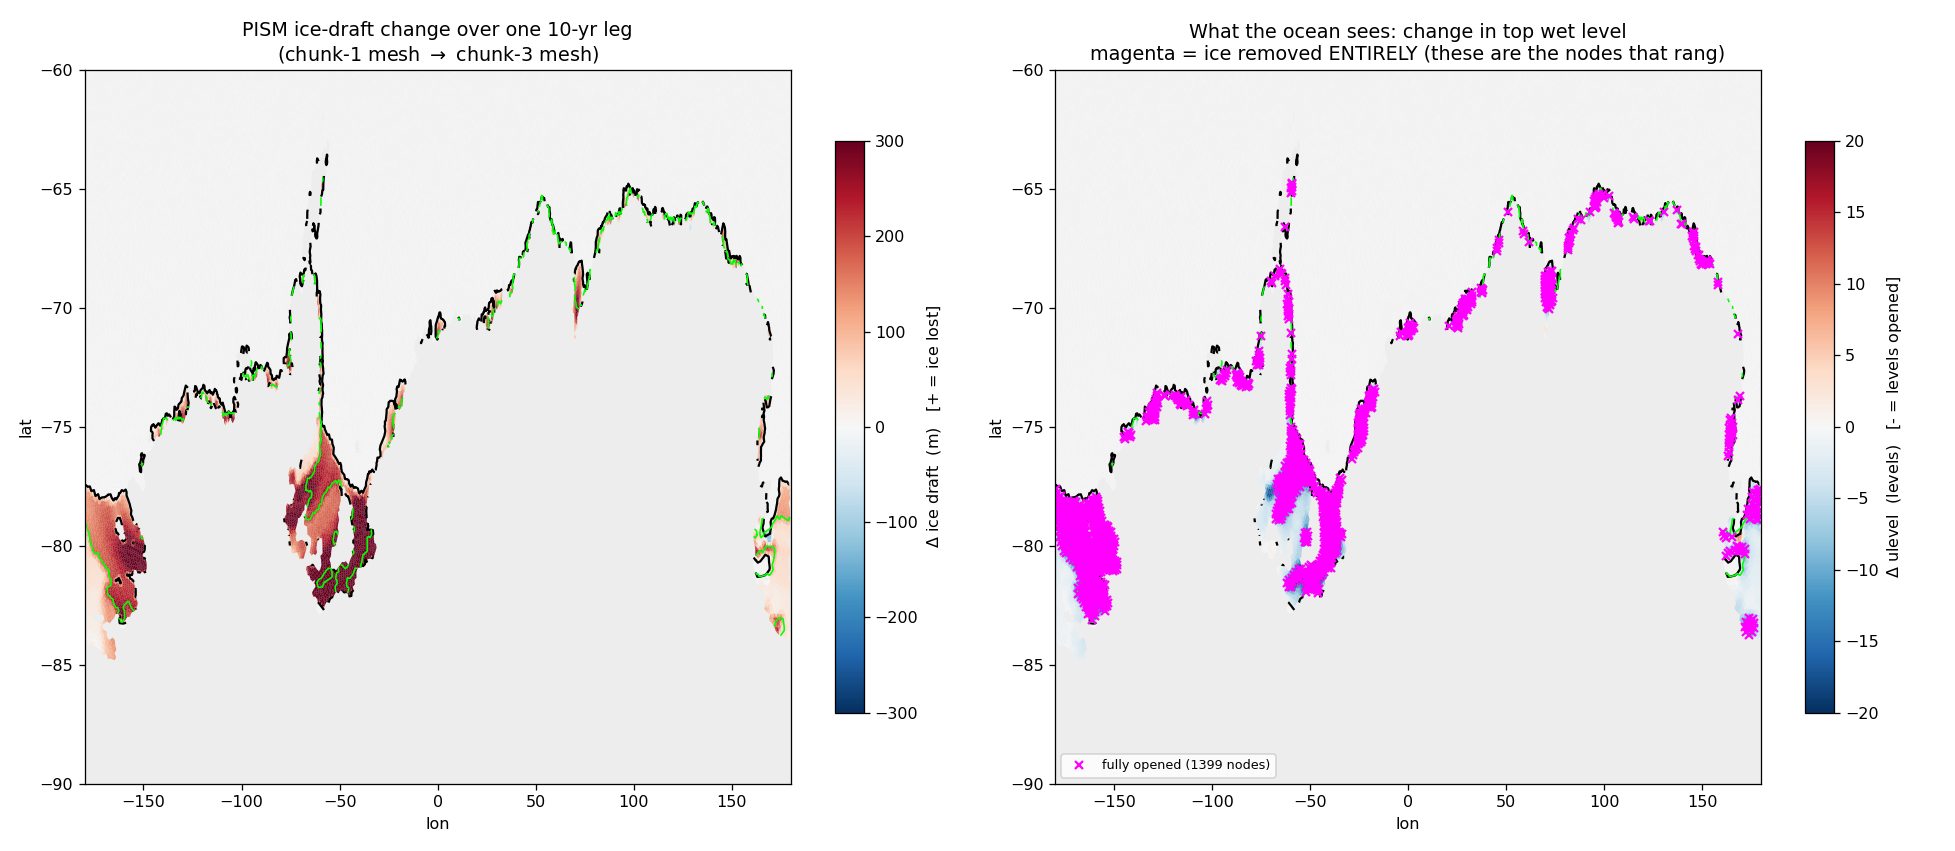
\includegraphics[width=\textwidth]{pism_change/pism_change_planview.png}\\
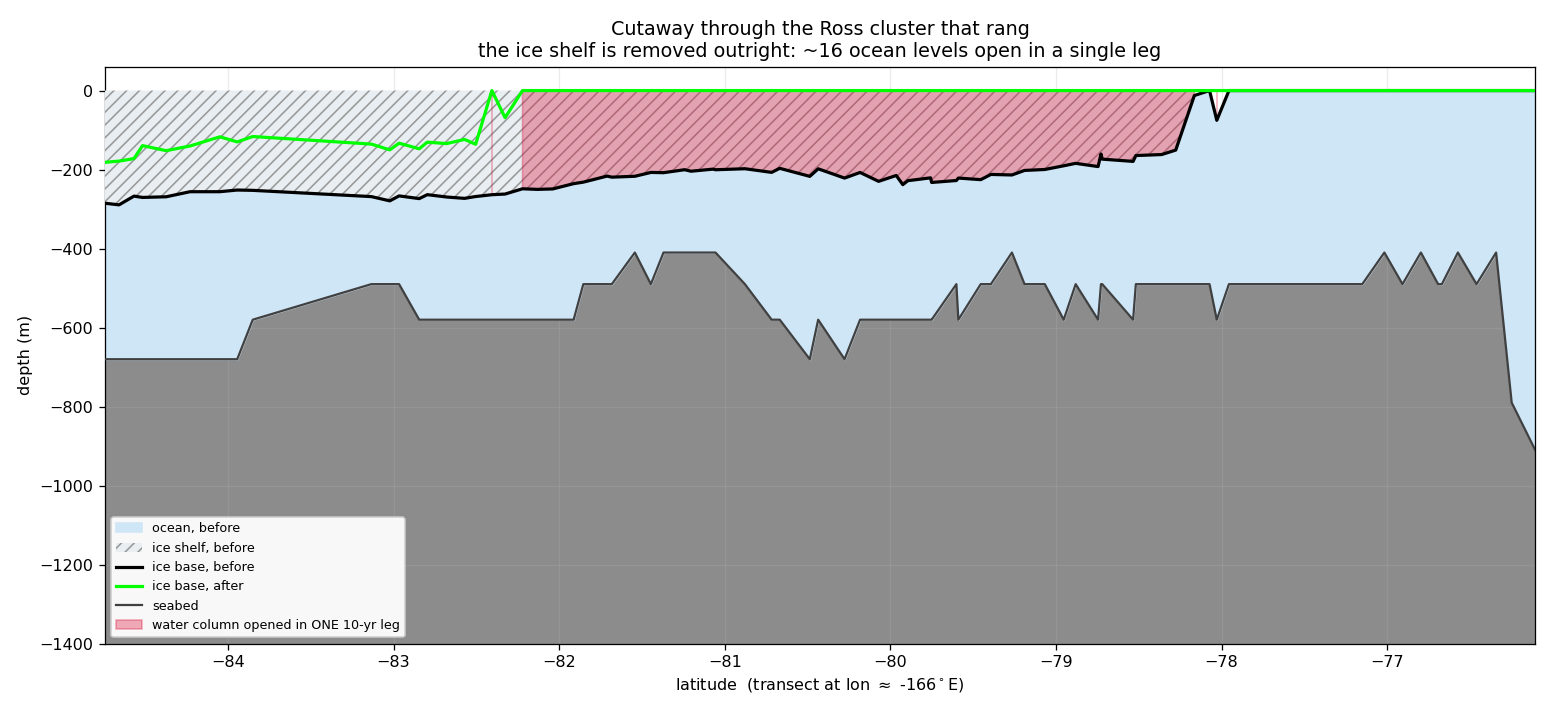
\includegraphics[width=0.92\textwidth]{pism_change/pism_change_section.png}
\caption{What Bug I did to PISM in one 10-year leg under surface-water forcing: 1399 nodes lose
their ice entirely (magenta ring around the whole margin), the Ross front retreats $\approx$440\,km
(section: ice base $-200\ldots-280$\,m $\to$ open ocean across four degrees of latitude).}
\label{fig:pism}
\end{figure}

\textbf{Fix (\code{93a207ee}): the DIRECT route.} PISM consumes FESOM's own cavity fluxes via
\code{-ocean given}: \code{fw}$\to$\code{shelfbmassflux} ($\times1000$, sign preserved),
\code{sst}$\to$\code{shelfbtemp}. One model owns the ice--ocean interface. The \code{-ocean given}
machinery existed all along but silently fell back to \code{th} because its input is a FESOM1.x-era
bundle FESOM2 never wrote; \code{fesom2ice} now synthesizes it (plus three exhumations of never-run
2D-path code: \code{3f07d7a2}, \code{74671c27}, \code{bb9d00c2}).

\subsection{Bug II --- the exchange weights scrambled the coupled ocean (2026-07-14)}\label{sec:bug2}

\begin{figure}[H]\centering
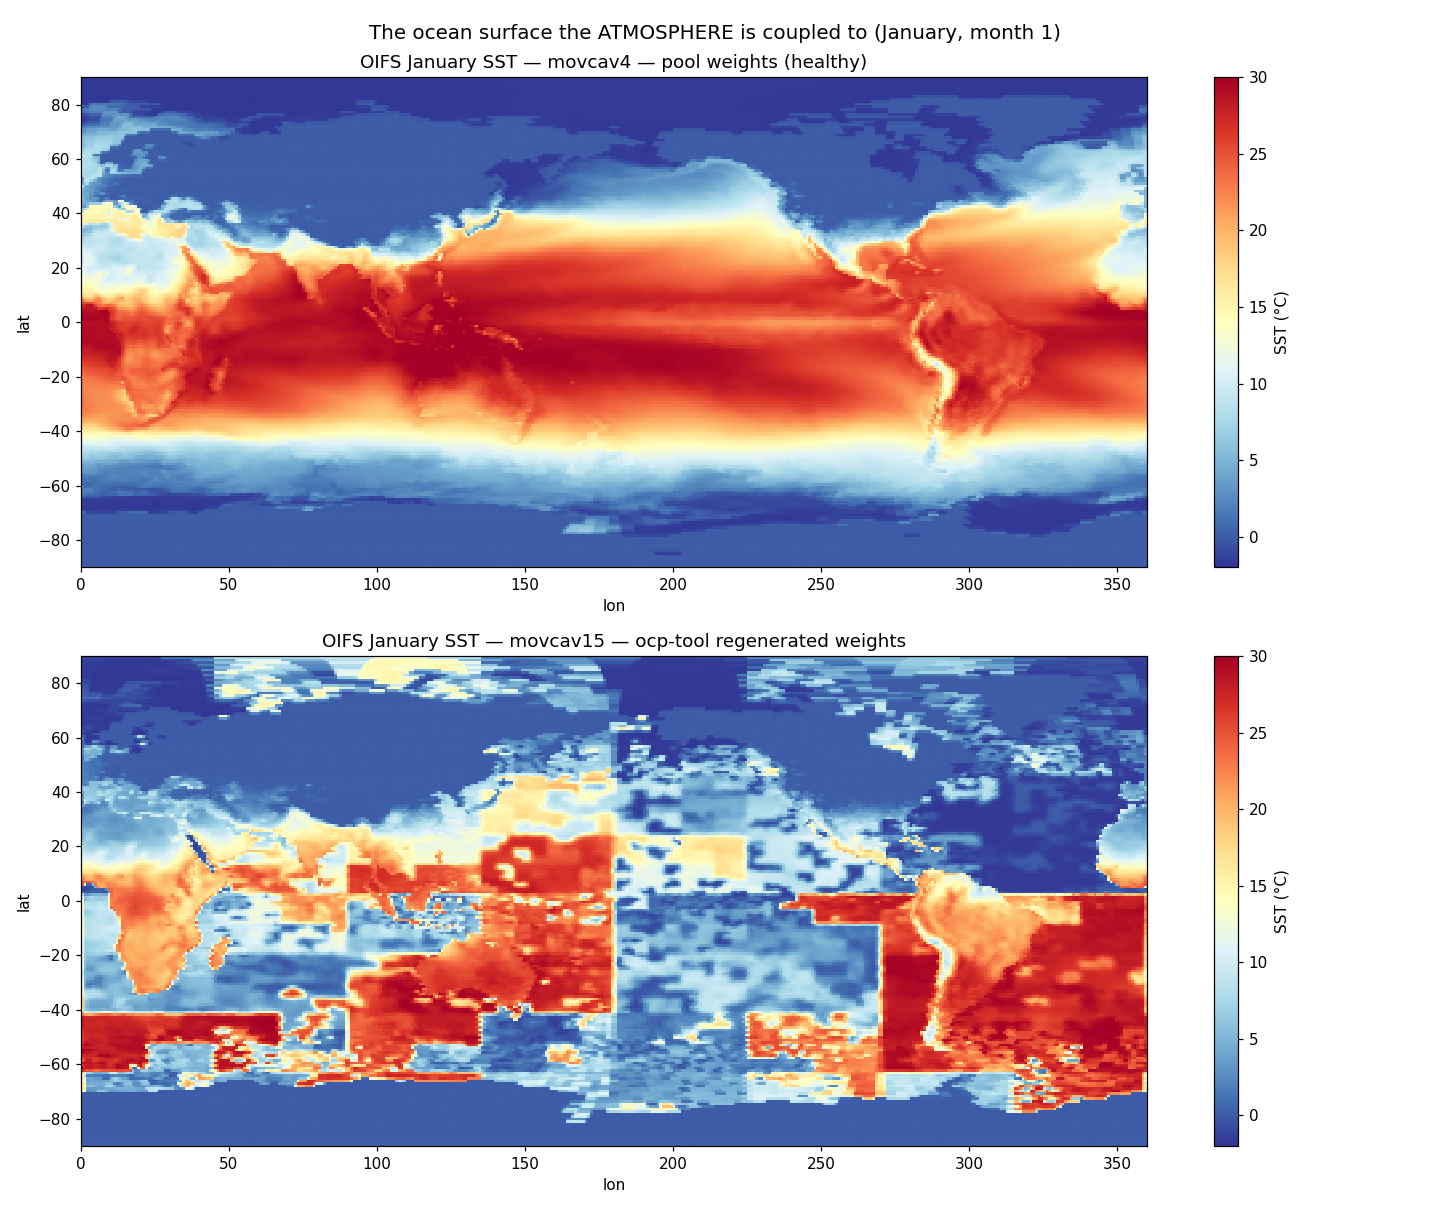
\includegraphics[width=\textwidth]{spp/sst_scramble_global.png}
\caption{\textbf{The picture that settles it.} January SST as OIFS holds it. Top: pool weights ---
textbook. Bottom: offline-engine weights --- a \emph{tile-translocated jigsaw}: tropical blocks at
$55^\circ$S, polar blocks on the equator, a seam at lon 180 where the node ordering breaks.}
\label{fig:jigsaw}
\end{figure}

FESOM exchanges coupling fields in \emph{partition (my\_list/rank) order}; the offline weight engine
(2026-06-17) built the feom geometry in \emph{nod2d.out order} (median displacement $58^\circ$).
Every submesh exchange was geographically tile-translocated (Fig.~\ref{fig:jigsaw}): OIFS saw
Weddell ice fraction 0.04 while FESOM had 0.95; global sea-ice death followed within months.

\textbf{Fix (\code{c21fe7c2}):} \code{permute\_feom\_to\_runtime.py} reorders the OASIS geometry to
runtime order (via \code{dist\_<nproc>/rpart.out}); \code{validate\_feom\_weights.py} applies every
weight file to real latitudes and \textbf{aborts the leg} above $1^\circ$ median error (nod2d-ordered
weights fail at 42--58$^\circ$, correct ones pass at $\le0.025^\circ$).

\subsection{Bug III --- the OASIS coupling restart was compound-scrambled (2026-07-14)}\label{sec:bug3}

\code{remap\_oasis\_restart.py} gathered in nod2d space, but its input and required output are both
\emph{runtime}-ordered: the emitted \code{rstos.nc} matched \emph{neither} ordering (correlation of
\code{sst\_feom} with the restart's own surface temperature: $+0.15$). OIFS's first coupling interval
saw 305\,K water under polar air --- a one-hour global jigsaw shock that nondeterministically
detonated the convection scheme (identical inputs crashed at hour 19, hour 458, or never).

\textbf{Fix (\code{abe56ee2}):} un-permute via the old mesh's \code{rpart.out} $\to$ gather $\to$
re-permute via the new mesh's; correlation now $+0.995$. Pool \code{rstos.nc} rebuilt.

%======================================================================
\subsection{The wave model's frozen coastline (2026-07-15)}\label{sec:wam}

Chunk-3 died deterministically at its first physics step in \code{voskin\_mod.F90:282} squaring
WAM's Stokes drift. WAM has no runtime tiling: its sea-point set is baked into
\code{wam\_grid\_tables} at preprocessing time and had never been regenerated. A cell that is ocean
per the regenerated lsm but land per WAM never receives wave data; the Stokes/Charnock fields are
srf-restart-carried, so a \emph{warm} start after a coastline change reads never-written storage
(cold starts zero-initialize --- why chunk-1 tolerates its 12 mismatch cells and historical lsm
changes never hit this). Chunk-3 had 125 mismatch cells. WAM itself was separately exonerated for
the Bug-IV crash family (a WAM-off run crashed identically).

\textbf{Fix: one-time maximal-ocean tables} (option A; tolerance patching rejected). WAM's sea-point
set was rebuilt from ETOPO1 with the southern limit extended $78\to85^\circ$S, then \emph{max-ocean
edited}: every cell the FESOM max-mesh can make wet --- open ocean or sub-shelf cavity --- is forced
to sea at its FESOM bottom depth (only ever adding ocean). 1277 cells opened (29\,555 $\to$ 30\,832
sea points), 283 of them south of $55^\circ$S: exactly the band a moving coastline walks through
(Fig.~\ref{fig:wammax}). The tables never change again, wave restarts stay index-compatible across
all future mesh changes, and WAM cold-starts once at the switch leg. Known cosmetic debt: the
max-ocean edit did not update the obstruction coefficients.

\begin{figure}[H]\centering
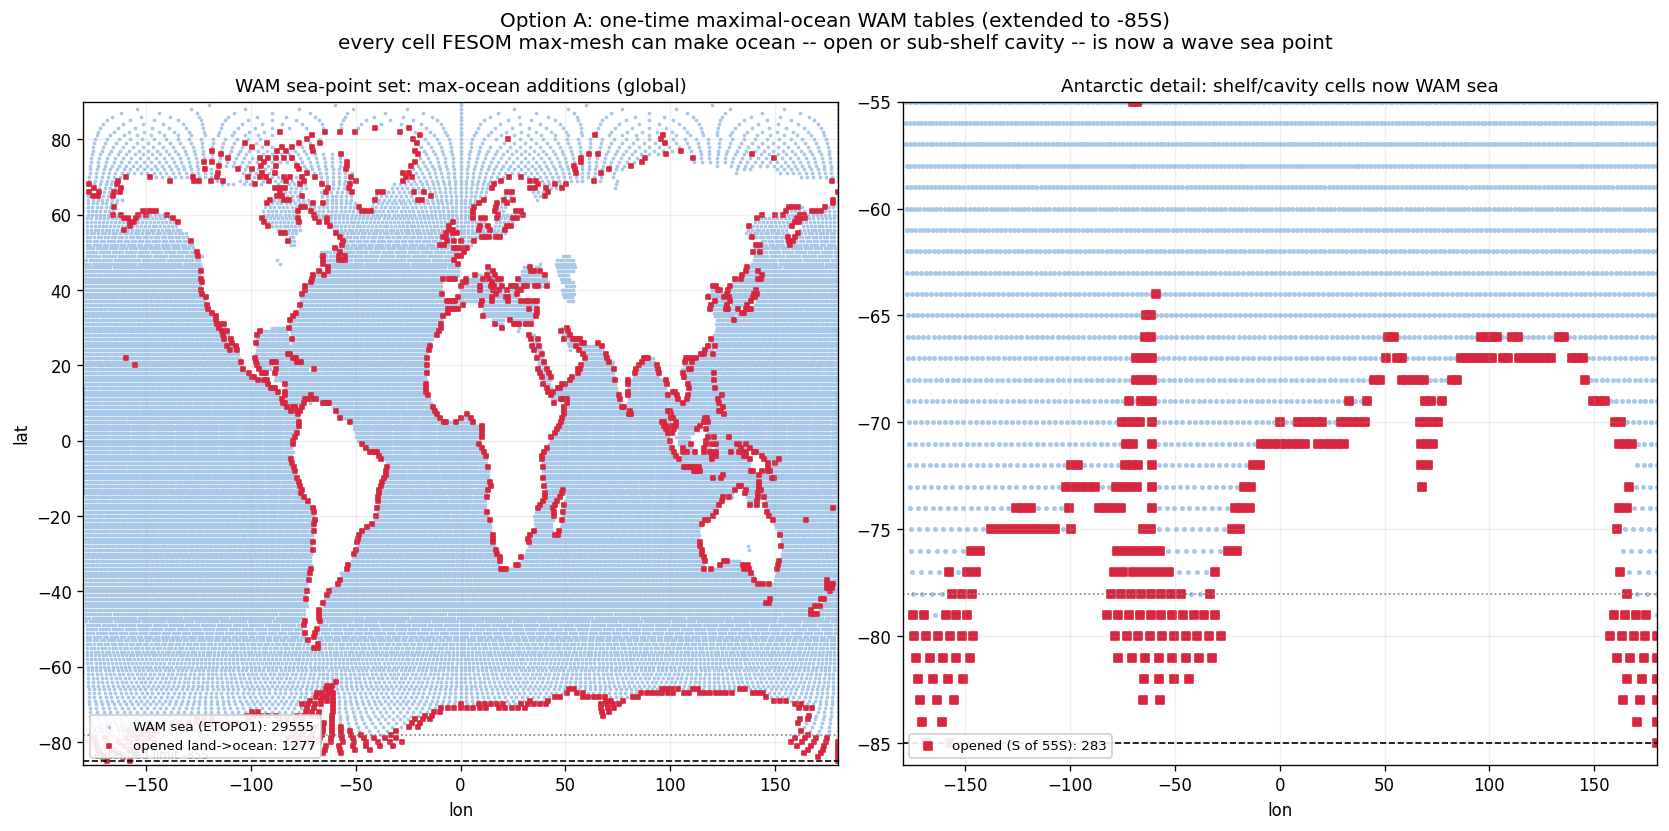
\includegraphics[width=\textwidth]{spp/wam_maxocean.png}
\caption{One-time maximal-ocean WAM tables (extended to $85^\circ$S). Blue: wave sea points from
ETOPO1. Red: cells opened land$\to$ocean because the FESOM max-mesh has a water column there.
Pre-registering them closes the WAM-Stokes route into \code{voskin:282}. (It does \emph{not} close
the line entirely: \code{voskin:282} later recurred through a different, in-step route ---
\S\ref{sec:voskin-inventory}.)}
\label{fig:wammax}
\end{figure}

\subsection{Bug IV --- the ice-surface-temperature coupling is architecturally unstable (2026-07-14$\to$16)}
\label{sec:bug4}

This is the mid-run OIFS crash family (\code{cubasen}/\code{vsurf}/\code{voskin} floating overflow,
random timing, polar/MIZ ranks). It survived three partial fixes before the root was found; the full
chain is worth recording because each layer was real, just not sufficient.

\paragraph{Layer 1: MIZ aliasing of the sent temperature.} FESOM sent raw \code{ist}; ice-free nodes
send the seawater freezing point, so the GAUSWGT cell blend in the marginal ice zone was dominated by
warm open water: OIFS's ice tile saw a surface tens of K too warm and returned a strongly negative
flux to the fully-iced nodes. Partial fix: concentration-weighted ist
(\code{ist$\cdot$a\_ice} $\div$ ci on ingest, the EC-Earth/NEMO convention behind
\code{ECE\_CPL\_NEMO\_WEIGHTED\_ICE}). Runs survived $3\times$ longer, still crashed.

\paragraph{Layer 2: the FESIM solve has no flux feedback within the coupling interval.}
FESIM's skin solve relaxes toward $t^{*}=T_f+\mathrm{a2ihf}\cdot\mathrm{zsniced}/\mathrm{con}$ with
the received flux \emph{frozen} for the hour and no d$Q$/d$T$ term: under insulation the equilibrium
runs away (measured floors 145--183\,K; excursions to $-954$\,K in one run). Partial fix: an
implicit flux linearization anchored at the transmitted temperature,
$Q(t)=\mathrm{a2ihf}+\lambda\,(t_{\mathrm{ref}}-t)$ with
$\lambda = 4\varepsilon\sigma t_{\mathrm{ref}}^3 + \lambda_{\mathrm{turb}} \approx 20$\,W/m$^2$/K
(the NEMO-family fallback derivative), energy-closed by booking the linearization heat to the ice
growth budget (fesom branch \code{awiesm3-implicit-ice-surftemp}, \code{38a558b5}). Dips became
bounded and self-recovering in most runs --- but not all.

\paragraph{Layer 3 (the root): the atmosphere's ice skin was never solved at all.}
Send-side instrumentation of \code{A\_Q\_ice} (term decomposition + tile state at every
$|Q|>1$\,kW/m$^2$ event) delivered the verdict:

\begin{itemize}
\item The received flux at cold FESOM nodes is \textbf{unphysical and anti-braking}: mean
  $-15.8$\,kW/m$^2$ below 150\,K (100\% negative), $-4.5$\,kW at 150--180\,K, recurring all year
  with the MIZ seasonal cycle --- at \textbf{49$^\circ$N on 0.1--0.5\,m ice with thin snow}
  (Okhotsk / St.\ Lawrence). Insulation is irrelevant there; no realistic $\lambda$ brakes kilowatts.
\item At the OIFS send, the generating cells have ice-tile fractions down to 0.04 and
  \textbf{tile skin temperatures of $\sim$204\,K under $\sim$275\,K maritime air}; the sensible +
  latent terms then reach $+17.8$\,kW/m$^2$ per tile area. With weighted-ist the tile skins were
  \emph{still} 189--204\,K at substantial tiles --- the cold temperature is genuine FESIM state,
  faithfully communicated.
\item The reason the skin can sit 80\,K below the air: \code{vlamsk\_mod.F90}, sea-ice tile, with
  \code{LNEMOSICOUP=.true.} (the default): \code{PLAMSK = 1e10} --- \textbf{the skin conductivity is
  set to infinity, pinning the tile skin to the prescribed (remapped FESOM) ice temperature}. The
  atmosphere's surface scheme was forbidden from solving its ice surface; it computed fluxes against
  whatever arrived through the remap.
\end{itemize}

The loop, in one line: FESIM's oscillating solve $\to$ remap $\to$ \emph{pinned} OIFS skin $\to$
kW fluxes against an unresolvable surface $\to$ remap $\to$ FESIM slams further --- a two-model
positive feedback closed through the marginal ice zone, metastable enough that identical
configurations coin-flipped between completing a year and dying at day 2 (runs movcav25--31:
raw/weighted $\times$ $\lambda\!=\!3.4/20$ $\times$ dirty/clean initial state --- every combination
crash-prone).

\textbf{Root fix: the coupled slab (\S\ref{sec:slab}).} Stop prescribing the atmosphere's ice skin
altogether; let OIFS solve it implicitly each timestep with conduction through the \emph{coupled}
FESOM ice and snow thickness. This removes the loop by construction while keeping the flux honest
about the actual ice state. Upstream note: mainline AWI-CM3 carries the same pinned-skin
architecture and therefore the same latent (if rarer) crash mode.

\subsection{Bug V --- iterative coupling never handed over to PISM (2026-07-16)}\label{sec:bug5}

The awiesm3$\to$PISM model switch is resolved at SimulationSetup init by reading the
\code{chunk\_date} file, whose path \code{esm\_runscripts/chunky\_parts.py} builds by \emph{raw
string concatenation of \code{general.base\_dir} before esm\_parser resolves variables}. A base\_dir
containing \code{\$\{user\}} was probed verbatim; the silent \code{isfile()} miss fell back to
``chunk 1, model 1'' --- awiesm3 self-resubmitted to its own final date and PISM never ran. Proven
by log comparison: identical resubmission command lines resolve to \code{Valid Model Names =
['pism']} under a literal base\_dir (movcav16 era) and to \code{['fesom','oifs',\ldots]} under
\code{\$\{user\}}.

\textbf{Fix (\code{d61297e8}):} \code{\_early\_resolve()} expands \code{\$\{\ldots\}} against
\code{general} (environment fallback) in all three chunk-file path builders. Regression-tested
against a real chunk file, and validated live: the first genuine awiesm3$\to$PISM handover of the
campaign (movcav27), and a full awiesm3$\to$PISM$\to$couple\_out$\to$chunk-3-couple\_in chain
(movcav29).

%======================================================================
\subsection{The coupled-slab architecture (2026-07-16/17)}\label{sec:slab}

The new division of labour: \textbf{OIFS owns the ice surface temperature; FESOM owns the ice
state.} OIFS's surface scheme solves the ice-tile skin implicitly within every atmosphere timestep
(full radiative + turbulent d$Q$/d$T$, finite skin conductivity), with slab conduction through the
coupled per-ice thickness and snow depth. FESOM's albedo still drives the radiation; FESIM's own ist
solve remains for its internal state (albedo, melt ponds) but is read by nobody --- the feedback
loop is cut by construction. The machinery is EC-Earth/KNMI heritage
(\code{ICESTATENEMO}, 2008; the SI3 branch of \code{callpar}) --- our contribution is wiring the
FESOM branch, which lacked only the thickness.

\paragraph{New exchange field.} FESOM sends \code{sit\_feom} = effective (grid-mean) ice thickness
\code{m\_ice} (o2a collection, \code{A\_Ice\_thickness});
\code{ECE\_FESIM\_GET\_ICE\_STATE} divides by the received ice fraction (standard
$\varepsilon$-guard) for the per-ice thickness the slab needs, falling back to the climatological
1.5\,m only where the cell has no significant ice. Snow thickness (\code{snt\_feom}) was already
exchanged and now actually reaches \code{surfseb} via \code{SURFL\%ZSNTICE}.

\paragraph{The switch set (verified in code, not inferred):}

\begin{center}
\begin{tabular}{@{}llp{8.6cm}@{}}
\toprule
switch & setting & verified effect \\
\midrule
\code{LNEMOSICOUP} & \textbf{.false.} & \code{vlamsk}: sea-ice tile skin conductivity becomes
  \emph{finite} (land-tile-style lookup) instead of $10^{10}$ --- the skin is genuinely solved by
  the SEB. The prior default pinned it to the prescribed ice temperature; this pin was the
  kilowatt engine of Bug IV. \\
\code{LNEMOLIMTEMP} & \textbf{.false.} & disables the hourly overwrite of OIFS's 4-layer ice
  temperature (\code{SP\_SB YTL}) from the FESOM ist ingest; the profile is OIFS-prognostic
  (ICMGG-initialized, restart-carried). FESOM's ist send becomes inert. \\
\code{LNEMOLIMTHK} & \textbf{.true.} & activates the \code{callpar} fill of
  \code{ZTHKICE/ZSNTICE} from the coupled fields --- the skin/top-layer conduction feels the real
  ice thickness and snow insulation. (The deep 4-layer discretization keeps its fixed depths;
  the skin conduction is the term that controls winter fluxes.) \\
\code{LMCCDYNSEAICE} & .true. & master enable; false force-resets the whole \code{LNEMOLIM*}
  family (\code{sumcc}). \\
\code{LNEMOLIMALB} & .true. (default) & FESOM's albedo drives OIFS radiation
  (\code{surfrad\_layer} $\to$ FESIM getter; raw--raw convention, consistent). \\
\code{ECE\_CPL\_NEMO\_WEIGHTED\_ICE} & .true. (inert) & only acted inside the disabled ist ingest. \\
FESOM \code{latm\_owns\_ist} & \textbf{.true.} & FESIM growth budget takes the atmosphere flux
  directly (\code{Qatmice=-a2ihf}, the ECHAM convention); qres/qcon/qlam booking off. \\
\bottomrule
\end{tabular}
\end{center}

\noindent
The \code{sumcc} guard ``\code{LNEMOSICOUP} without \code{LNEMOLIMTEMP} does not make sense''
correctly enforces that a pinned skin requires a prescribed temperature; our mode flips both off.
In one sentence: \emph{before, OIFS's ice surface was a mirror bolted to whatever FESOM's
oscillating solve sent; now it is a real solved surface conducting through FESOM's actual ice and
snow.}

\paragraph{Validated (movcav33).} The first coupled-slab run completed its year crash-free and
handed over to PISM. With the instrumentation still armed: kW-scale send events at real ice tiles
went from 1410--1930 per run to \textbf{zero} (117 residual events are all phantom slivers with
ice fraction $\sim10^{-7}$, a \code{ZMASK} threshold cosmetic); event tile skins moved from
189--212\,K into the physical 247--265\,K range (Fig.~\ref{fig:senddbg}); the fluxes FESOM
receives at its coldest nodes are $-63\ldots-80$\,W/m$^2$ (textbook polar values, was
$-10$\,kW), and FESIM's internal temperature tracks its anchor to $<0.1$\,K.

\begin{figure}[H]\centering
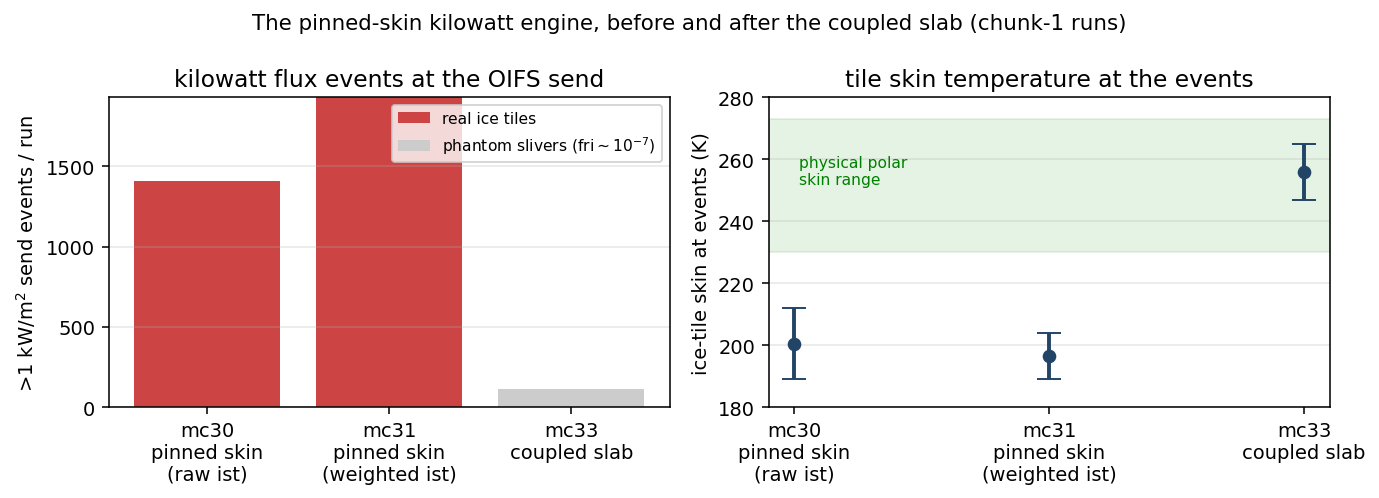
\includegraphics[width=0.9\textwidth]{seaice/senddbg_collapse.png}
\caption{The kilowatt engine, before and after. Left: $>$1\,kW/m$^2$ events at the OIFS send per
chunk-1 run. Right: the ice-tile skin temperature at those events --- pinned-skin runs sit 60--80\,K
below the physical range; the solved skin cannot.}
\label{fig:senddbg}
\end{figure}

%======================================================================
\subsection{First fruits of the clean decade: cavity melt against observations (2026-07-17)}\label{sec:melt}
The chunk-1 year that forced the first clean PISM decade, split by sector and set against the
satellite record (Rignot et al.\ 2013; Adusumilli et al.\ 2020):

\begin{center}
\begin{tabular}{@{}lrrrr@{}}
\toprule
sector & observed & \multicolumn{3}{c}{movcav33 chunk-1 (m\,w.e./yr)} \\
       & (m\,ice/yr) & mean & median & nodes \\
\midrule
Filchner--Ronne          & 0.3--0.4        & 0.89 & \textbf{0.20} & 1085 \\
Ross                     & $\sim$0.1       & 0.90 & \textbf{0.31} & 1075 \\
Amundsen--Bellingshausen & 14--27 (PIG 16) & 7.8  & 6.4  & 229 \\
Antarctic Peninsula      & 0.4--3.8        & 7.5  & 4.4  & 186 \\
Wilkes (Totten sector)   & 4.7--9.1        & 8.3  & 6.4  & 296 \\
Amery                    & 0.6--0.7        & 4.0  & 3.3  & 128 \\
E.\ Weddell / Dronning Maud & 0.3--0.9     & 4.4  & 3.5  & 287 \\
\midrule
circum-Antarctic         & 0.8 $\pm$ 0.7   & 2.84 & 0.79 & 3286 \\
\bottomrule
\end{tabular}
\end{center}

\noindent
The cold/warm dichotomy that dominates the observations is reproduced: the cold-cavity giants sit
at 0.2--0.3\,m/yr medians while the warm sectors run 4--8, and 13\% of the cavity area refreezes
(marine ice, as observed under Ronne/Amery). Residual biases: the East Antarctic coastal sectors
(Dronning Maud, Amery) run $\sim$5$\times$ warm, and the Amundsen runs $\sim$2$\times$ cold ---
both worth revisiting once multi-year coupled statistics exist. Caveats: node statistics
(unweighted), m\,w.e.\ vs the observations' m\,ice ($\times$0.92), one coupled year, and PISM's
initial geometry carries reduced versions of the big shelves. For scale: the jigsaw-era coupling
produced 28\,m/yr.


\subsection{The increment test crashes, twice --- and passes (2026-07-17/18)}\label{sec:zerowater}

The first chunk-3 leg --- awiesm3 on the PISM-changed 208\,438-node mesh, stage 6/6 --- absorbs
the mesh change and runs for weeks of model time before FESOM dies of an SSH explosion
($\eta$ jumping $\pm 40$\,m in one step at the Antarctic Peninsula tip; day 19--51 depending
on MPI reduction order --- the state is metastable). The autopsy was cheap for two reasons:
the leg costs 3--4 minutes of wall time, and a temporary XIOS file group with
\code{sync\_freq="1d"} flushes daily fields to disk as they complete, so even a crashed run
leaves full evidence (default XIOS files sync only on close: 51 days of output, zero
records). The hunt found \emph{two independent bugs}, stacked at the same place.

\begin{figure}[H]
\centering
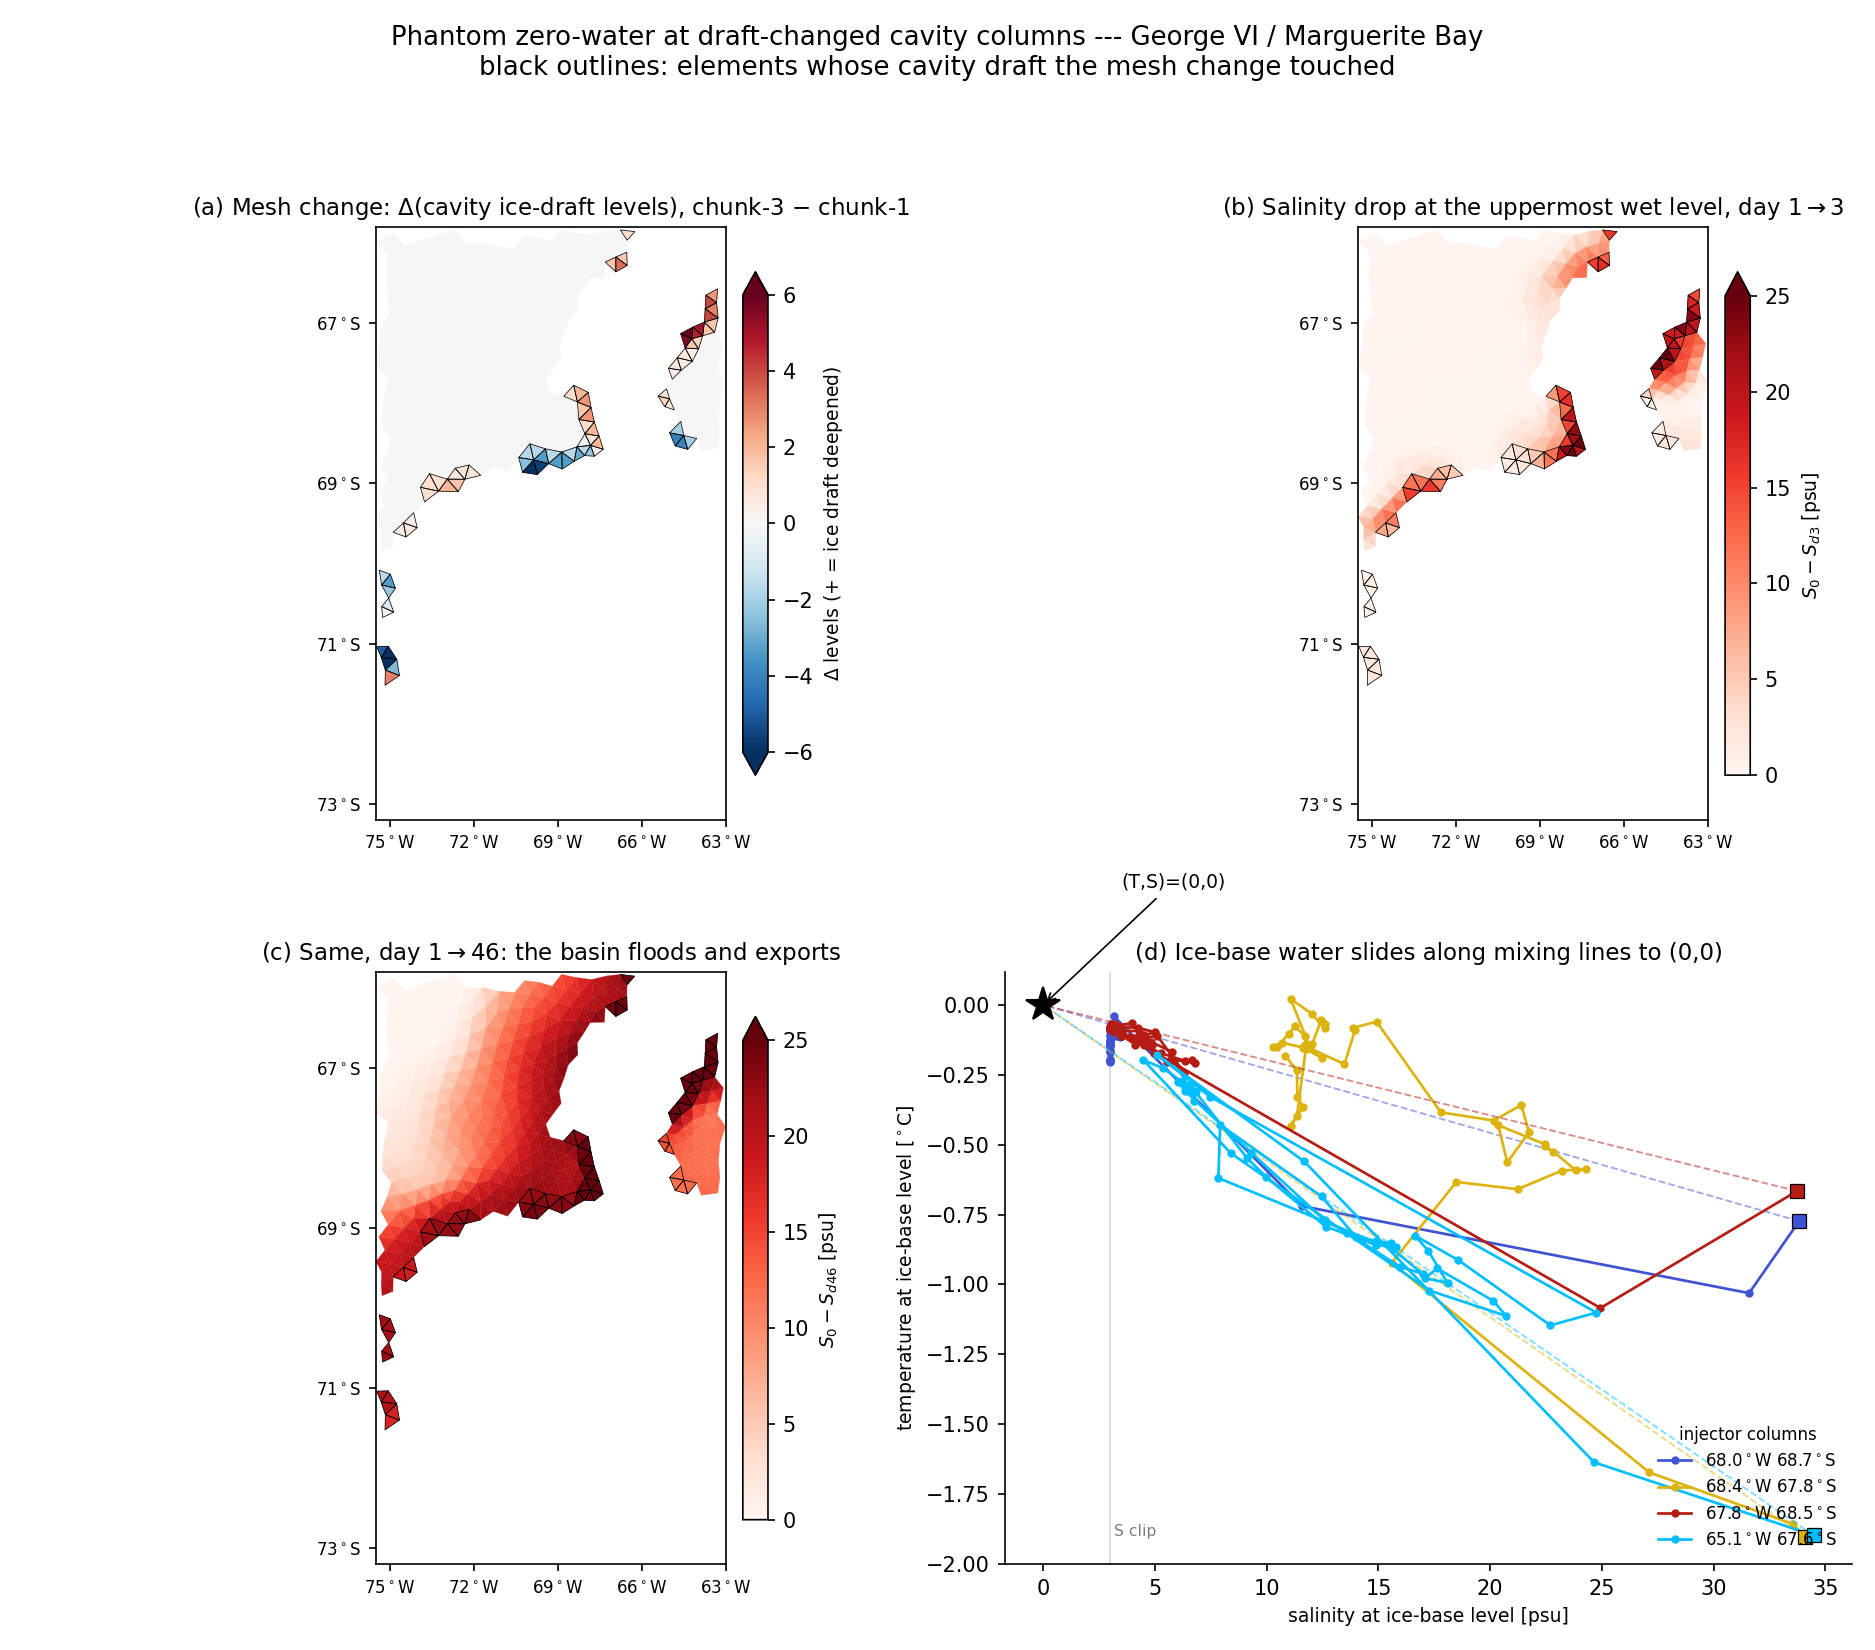
\includegraphics[width=\textwidth]{zero_water_george6.png}
\caption{Bug VI seen in one basin (George VI / Marguerite Bay; black outlines = the 73
elements whose cavity draft the mesh change touched). (a) The mesh change: $\pm$1--6 cavity
levels. (b) By day 3 the uppermost-wet-level salinity has dropped up to 25\,psu \emph{exactly
on the outlined elements}. (c) By day 46 the basin has flooded and exports along the coast.
(d) The fingerprint: $(S,T)$ at the ice-base level slides along the mixing lines toward
$(0,0)$ with \emph{identical} T- and S-replacement fractions --- not a flux (surface
freshwater is $50\times$ too small and negative), but a \emph{multiplicative drain}: both
tracers lose the same fraction of their value every step.}
\label{fig:zerowater}
\end{figure}

\subsubsection*{Bug VI --- the layer-thickness mismatch drain}
The remapped restart carries \code{hnode} inherited from the old mesh's zstar state (e.g.\
9.964\,m where a formerly ice-free column scaled its layers with $\eta$). At runtime,
cavity columns and their open-ocean edge ring (\code{ulevels\_nod2D\_max>1}) keep layer
thicknesses \emph{fixed at the mesh nominal} (10.000\,m) and are excluded from the per-step
\code{hnode}$\leftrightarrow$\code{hnode\_new} sync --- so the mismatch is immortal. FESOM's
tracer T$^{*}$ update applies
$\mathrm{values}\cdot(\code{hnode}-\code{hnode\_new})/\code{hnode\_new}$ every step: a
$-0.36\%$/step multiplicative drain on $T$ \emph{and} $S$. Per-operator probes at a Getz
injector column measured $-0.1226$\,psu/step against a predicted
$33.64\times0.0036=-0.1224$; an unchanged FRIS control column measured exactly zero. At
free-surface nodes next to the cavity edge the drain even \emph{accelerates}: $\eta$ grows,
the nominal-vs-restart gap grows with it. \textbf{Fix} (FESOM,
\code{restart\_thickness\_ale}): after the restart read, force \code{hnode} at the whole
excluded class back to the fixed nominal and rebuild the depth arrays. Validated by
intervention: the drain vanished ($+0.0002$/step), day-1 fields healthy.

\subsubsection*{Bug VII --- the drowned island}
With Bug VI fixed the run survived longer but still exploded at the Peninsula tip, $\eta$
climbing a steady $+0.11$\,m/day. The reason is geometric, not numeric
(Figs.~\ref{fig:island}, \ref{fig:islandanat}): the ice2fesom regrid remapped PISM's \emph{categorical} mask
\textbf{bilinearly} --- a few-cell island surrounded by mask-4 ocean smears to
$\approx$3.x, rounds to ocean, and is deleted from the submesh. PISM's own bed there is
$+38$ to $+218$\,m above sea level: bedrock island, regardless of ice. (The island entered
the campaign \emph{bare} --- the spinup state carries 0.0\,m of ice on all ten cells; a
thin 0.1--0.4\,m cap has been \emph{growing} during the coupled decades. A second,
independent deletion path was found while examining it: PISM encodes ice-free bedrock as
mask$=$0, which the node classifier silently defaulted to ocean; fixed --- bare bedrock
above sea level is land.) The ocean then drives a runaway coastal jet where a coastline should be.
\textbf{Fix} (ice2fesom): remap the categorical mask nearest-neighbour; rebuild the mask=5
outside-domain marker (which \code{remapnn} extrapolation would erase) from a bilinear
domain indicator. Continuous fields stay bilinear.

\begin{figure}[H]
\centering
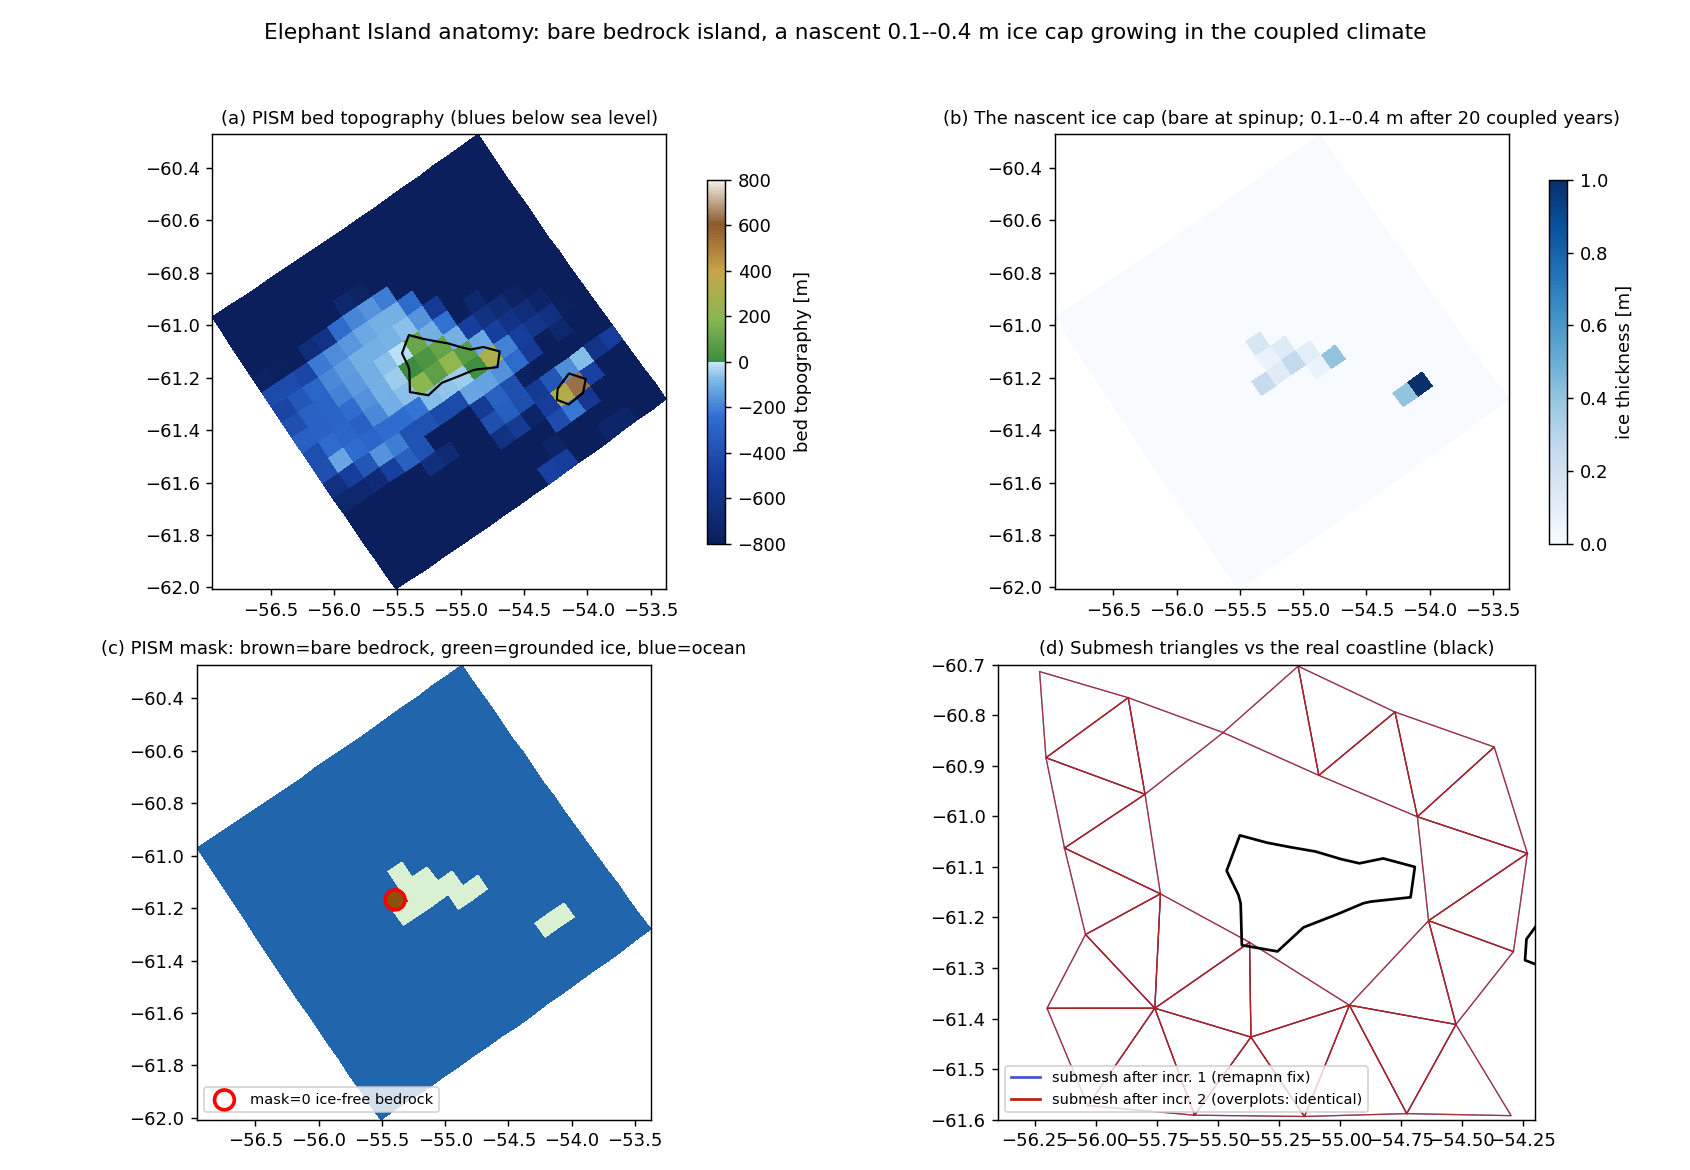
\includegraphics[width=\textwidth]{elephant_island_anatomy.png}
\caption{Elephant Island anatomy. (a) PISM bed topography, ETOPO-style colors: a genuine
bedrock island ($+4$ to $+297$\,m) on its shallow platform, Clarence's peak to the
southeast. (b) The \emph{nascent} ice cap: bare at spinup, 0.1--0.4\,m grown over 20
coupled years (DEBM accumulates here). (c) The PISM mask; the red circle is the single
mask$=$0 (ice-free bedrock) cell that exposed the classifier hole. (d) The submesh renders
the island identically after increments 1 and 2 --- the nearest-neighbour fix holds.}
\label{fig:islandanat}
\end{figure}

\begin{figure}[H]
\centering
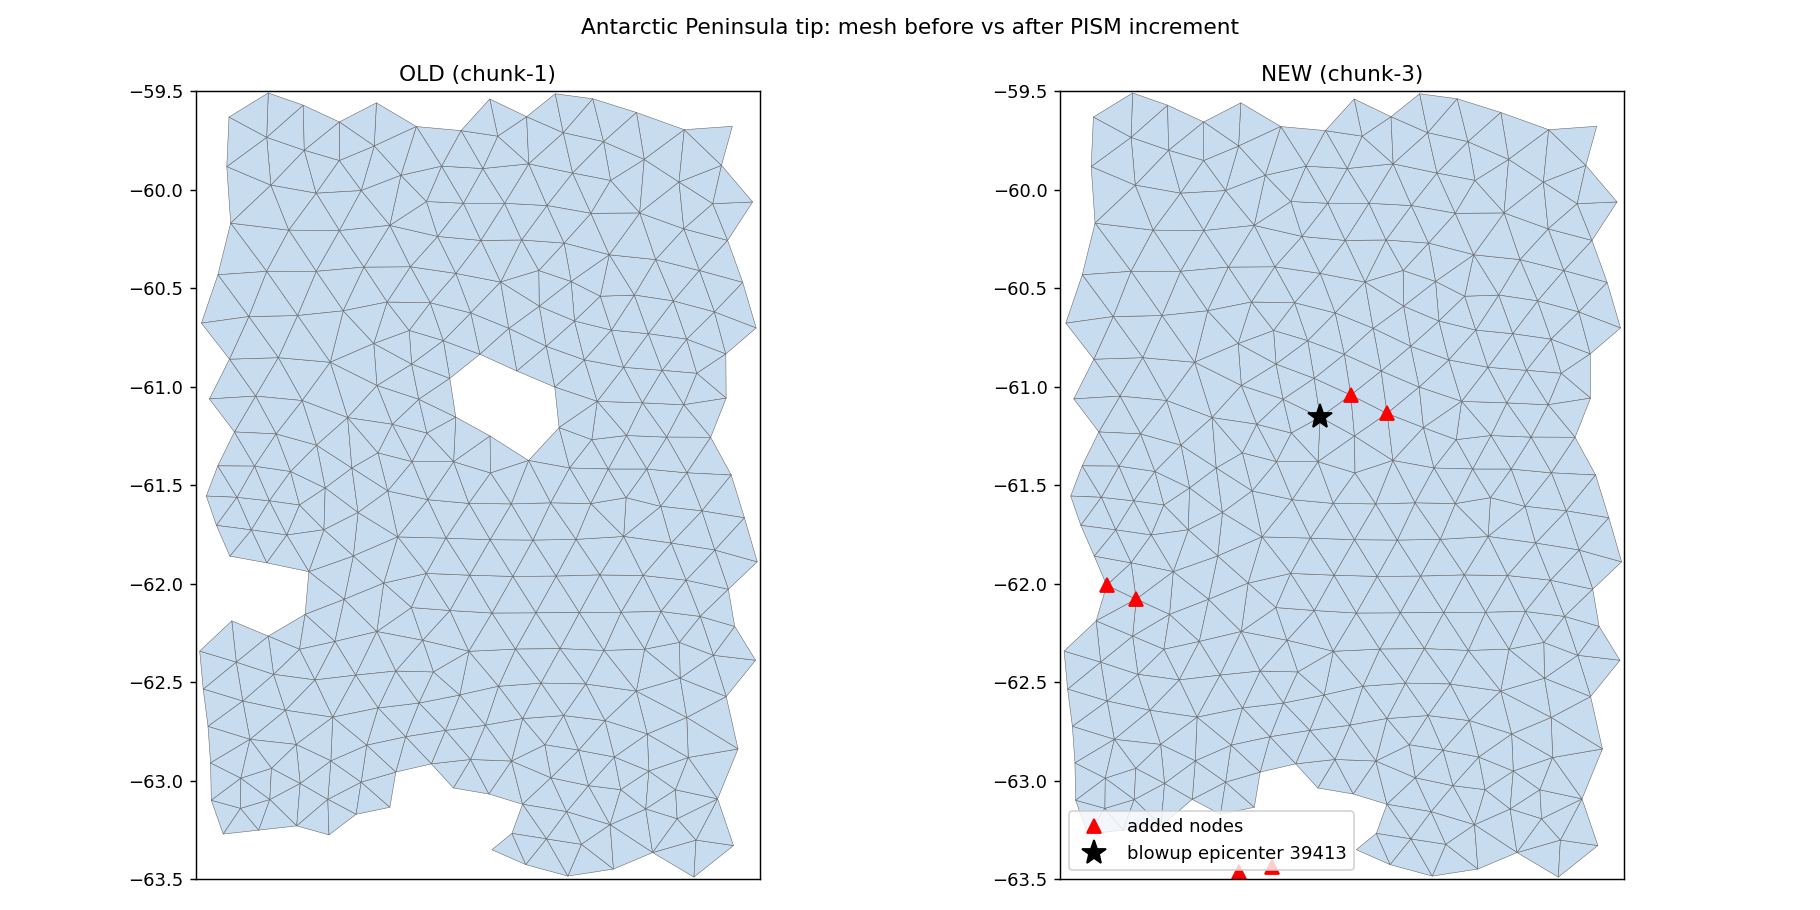
\includegraphics[width=\textwidth]{elephant_island_drowned.png}
\caption{Bug VII. Left: the chunk-1 mesh has Elephant Island (the hole at
$55.4^{\circ}$W, $61.1^{\circ}$S) and the Clarence/Gibbs notch. Right: after the PISM decade
the bilinear mask remap has rounded both islands to ocean --- the added nodes (red) fill
them in, and the blowup epicenter (star) sits exactly on the drowned island.}
\label{fig:island}
\end{figure}

\textbf{Ruled out by measurement} (each was a plausible suspect): surface freshwater fluxes;
OIFS runoff/calving and the \code{ECE\_LANDICE} snow cap; the OASIS \code{feom} masks; the
remapped $T/S$ state (freezing cap ran: 1137 columns); mesh-file level-range consistency
(zero violations); the zero-filled dry restart levels (padding them --- kept as a permanent
hygiene pass --- reproduced the crash bitwise); and the vertical-advection top boundary
(cavity guards in both the implicit and explicit schemes changed nothing --- see
\S\ref{sec:falsified}). The couple\_in warning about a missing
\code{cap\_new\_cavity\_temp.py} is a red herring: the freezing cap runs as Fortran inside
the remap binary.

\subsubsection*{The increment test passes}
With both fixes, movcav33 chunk-3 completed the full year 1901 on the changed mesh
(25\,min wall, no blowup; the Peninsula node's SSH wanders seasonally instead of pumping)
and handed over to the chunk-4 PISM decade unattended --- \textbf{stage 6/6 closed}. The
long run movcav34 (10 awiesm3 years / 100 PISM years) then repeated chunks 1--4 cleanly on
the \emph{minimal} build (hnode fix only; the advection guards were reverted after being
falsified). Fixes are committed: FESOM \code{awiesm3-implicit-ice-surftemp}, esm\_tools
\code{development\_interactiv\_mesh\_awiesm3}.

\subsubsection*{The next problem: the second increment and the hygiene overreach (2026-07-18)}
movcav34's chunk-5 (year 1902, after 20 PISM years) blew up at day 16 at the western Ross
front, where the second increment opened cavity columns wholesale (ulev $13\to1$) amid a
506-node ice advance. The new coastline there was structurally rotten: 24 nodes within
$1.5^{\circ}$ of the epicenter held by $\le$3 elements, including an 18-levels-under-ice
cavity column held by exactly two triangles. A \emph{coastline-hygiene sweep} was added to
the submesh tool (iteratively remove ice-domain nodes held by $\le$2 elements) and the chain
then ran unattended through year 1911 and 120 PISM years --- eleven further increments
without a FESOM blowup, ending only in a recurrence of the old OIFS \code{voskin} overflow
at chunk 13.

\textbf{The overreach.} At wrap-up the evolution diagnostics exposed the truth
(Figs.~\ref{fig:evol}, \ref{fig:fris}): the hygiene sweep had \emph{cascaded through the
narrow cavity bands} --- fringing shelves and cavity margins are exactly the few-element-wide
structures the criterion eats rim-inward --- and every post-1902 submesh carries only
14--111 cavity nodes instead of $\sim$2600. The node classifier was healthy (2223 shelf
nodes flagged); the lake floodfill removed only 35 elements; the sweep itself did the
damage. \textbf{The eleven ``stable'' legs ran with the ice-shelf cavities amputated ---
stability by amputation, and every result from movcav34 after chunk 4 is
\textcolor{red}{TAINTED}.} The sweep was reverted the same day (commit \code{ca0641b2}
reverts \code{680daa55}).

\begin{figure}[H]
\centering
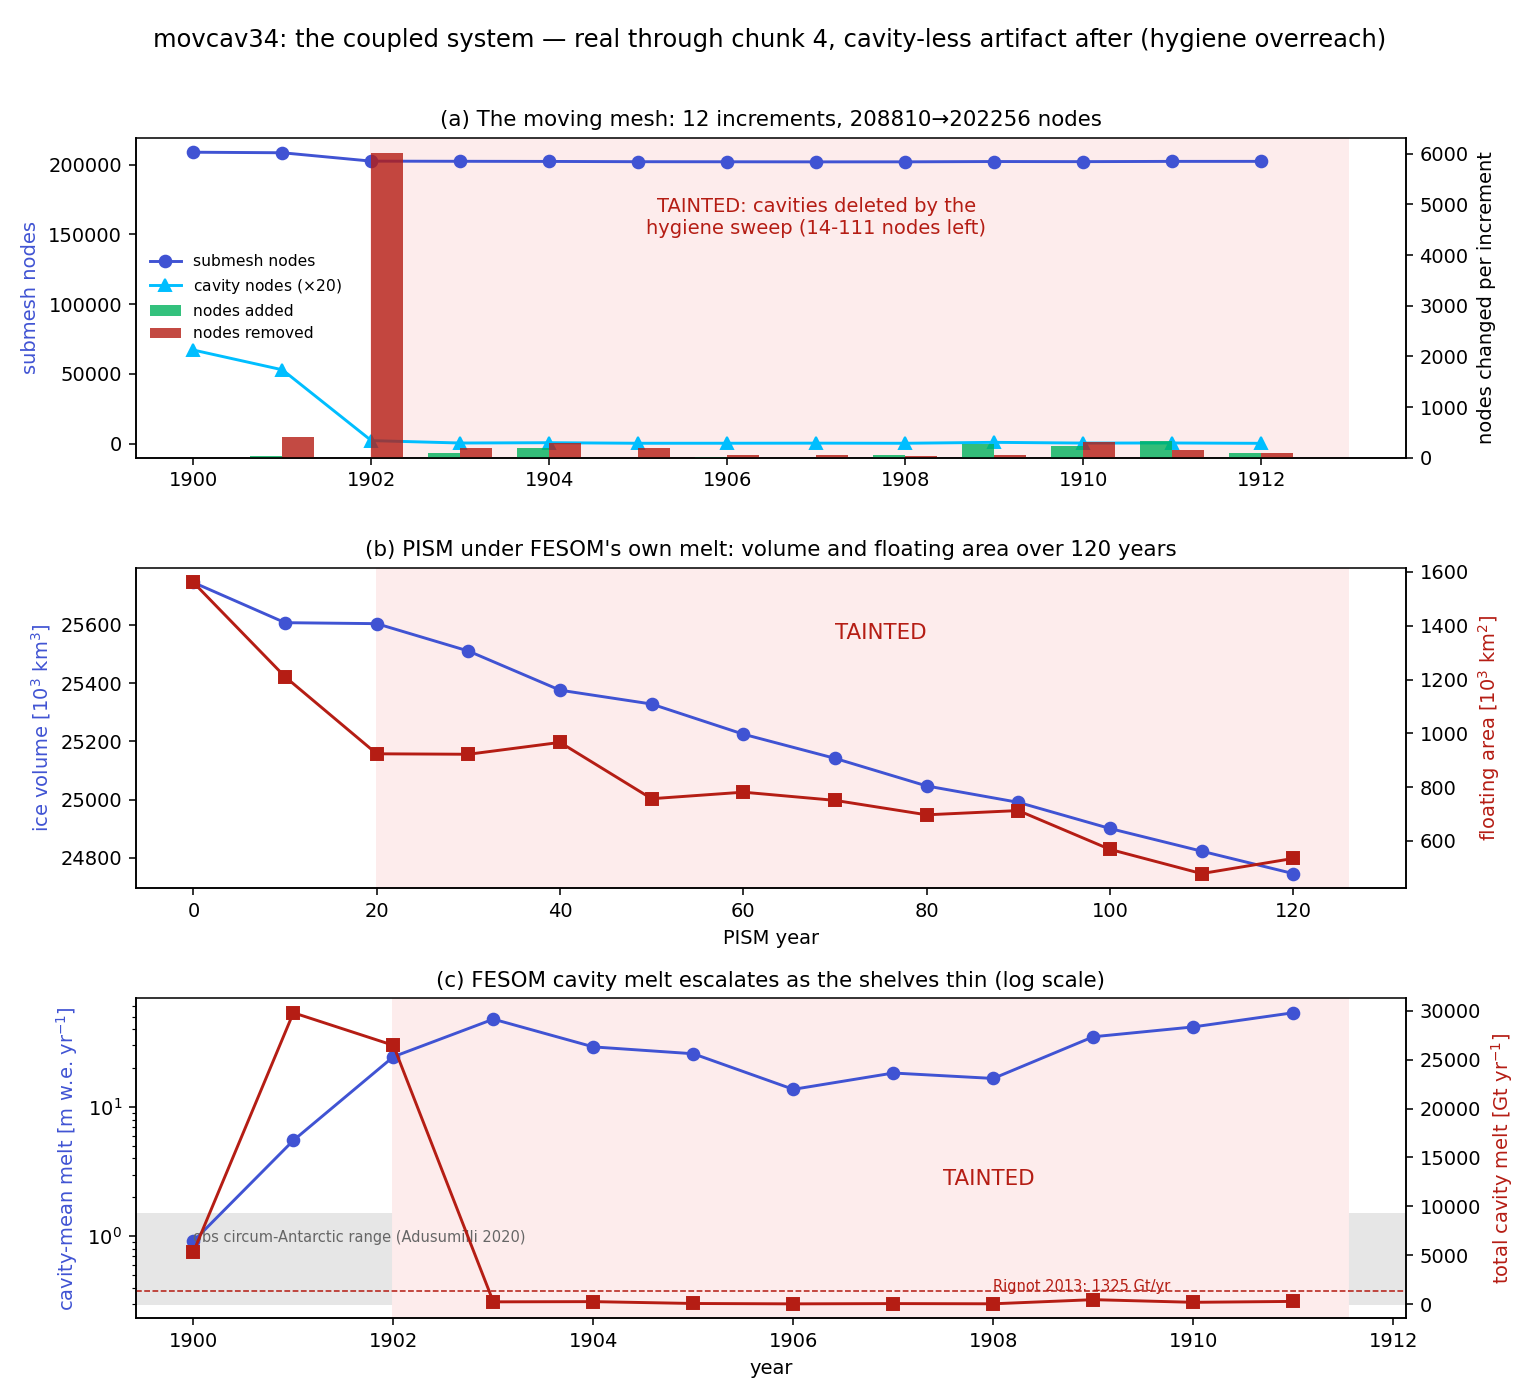
\includegraphics[width=\textwidth]{movcav34_evolution_timelines.png}
\caption{The movcav34 production run, honest version. (a) Submesh and cavity-node counts per
increment: the collapse from 2647 to 111 cavity nodes at the 1902 mesh is the hygiene
amputation. (b) PISM volume and floating area over 120 years: the decline is real coupled
melt through year 20, then continues under forcing computed from an essentially cavity-less
ocean. (c) Cavity-mean and total melt per leg (log scale): the escalation beyond
$\sim$1902 samples only the few surviving cavity slivers. Red shading = tainted.}
\label{fig:evol}
\end{figure}

\begin{figure}[H]
\centering
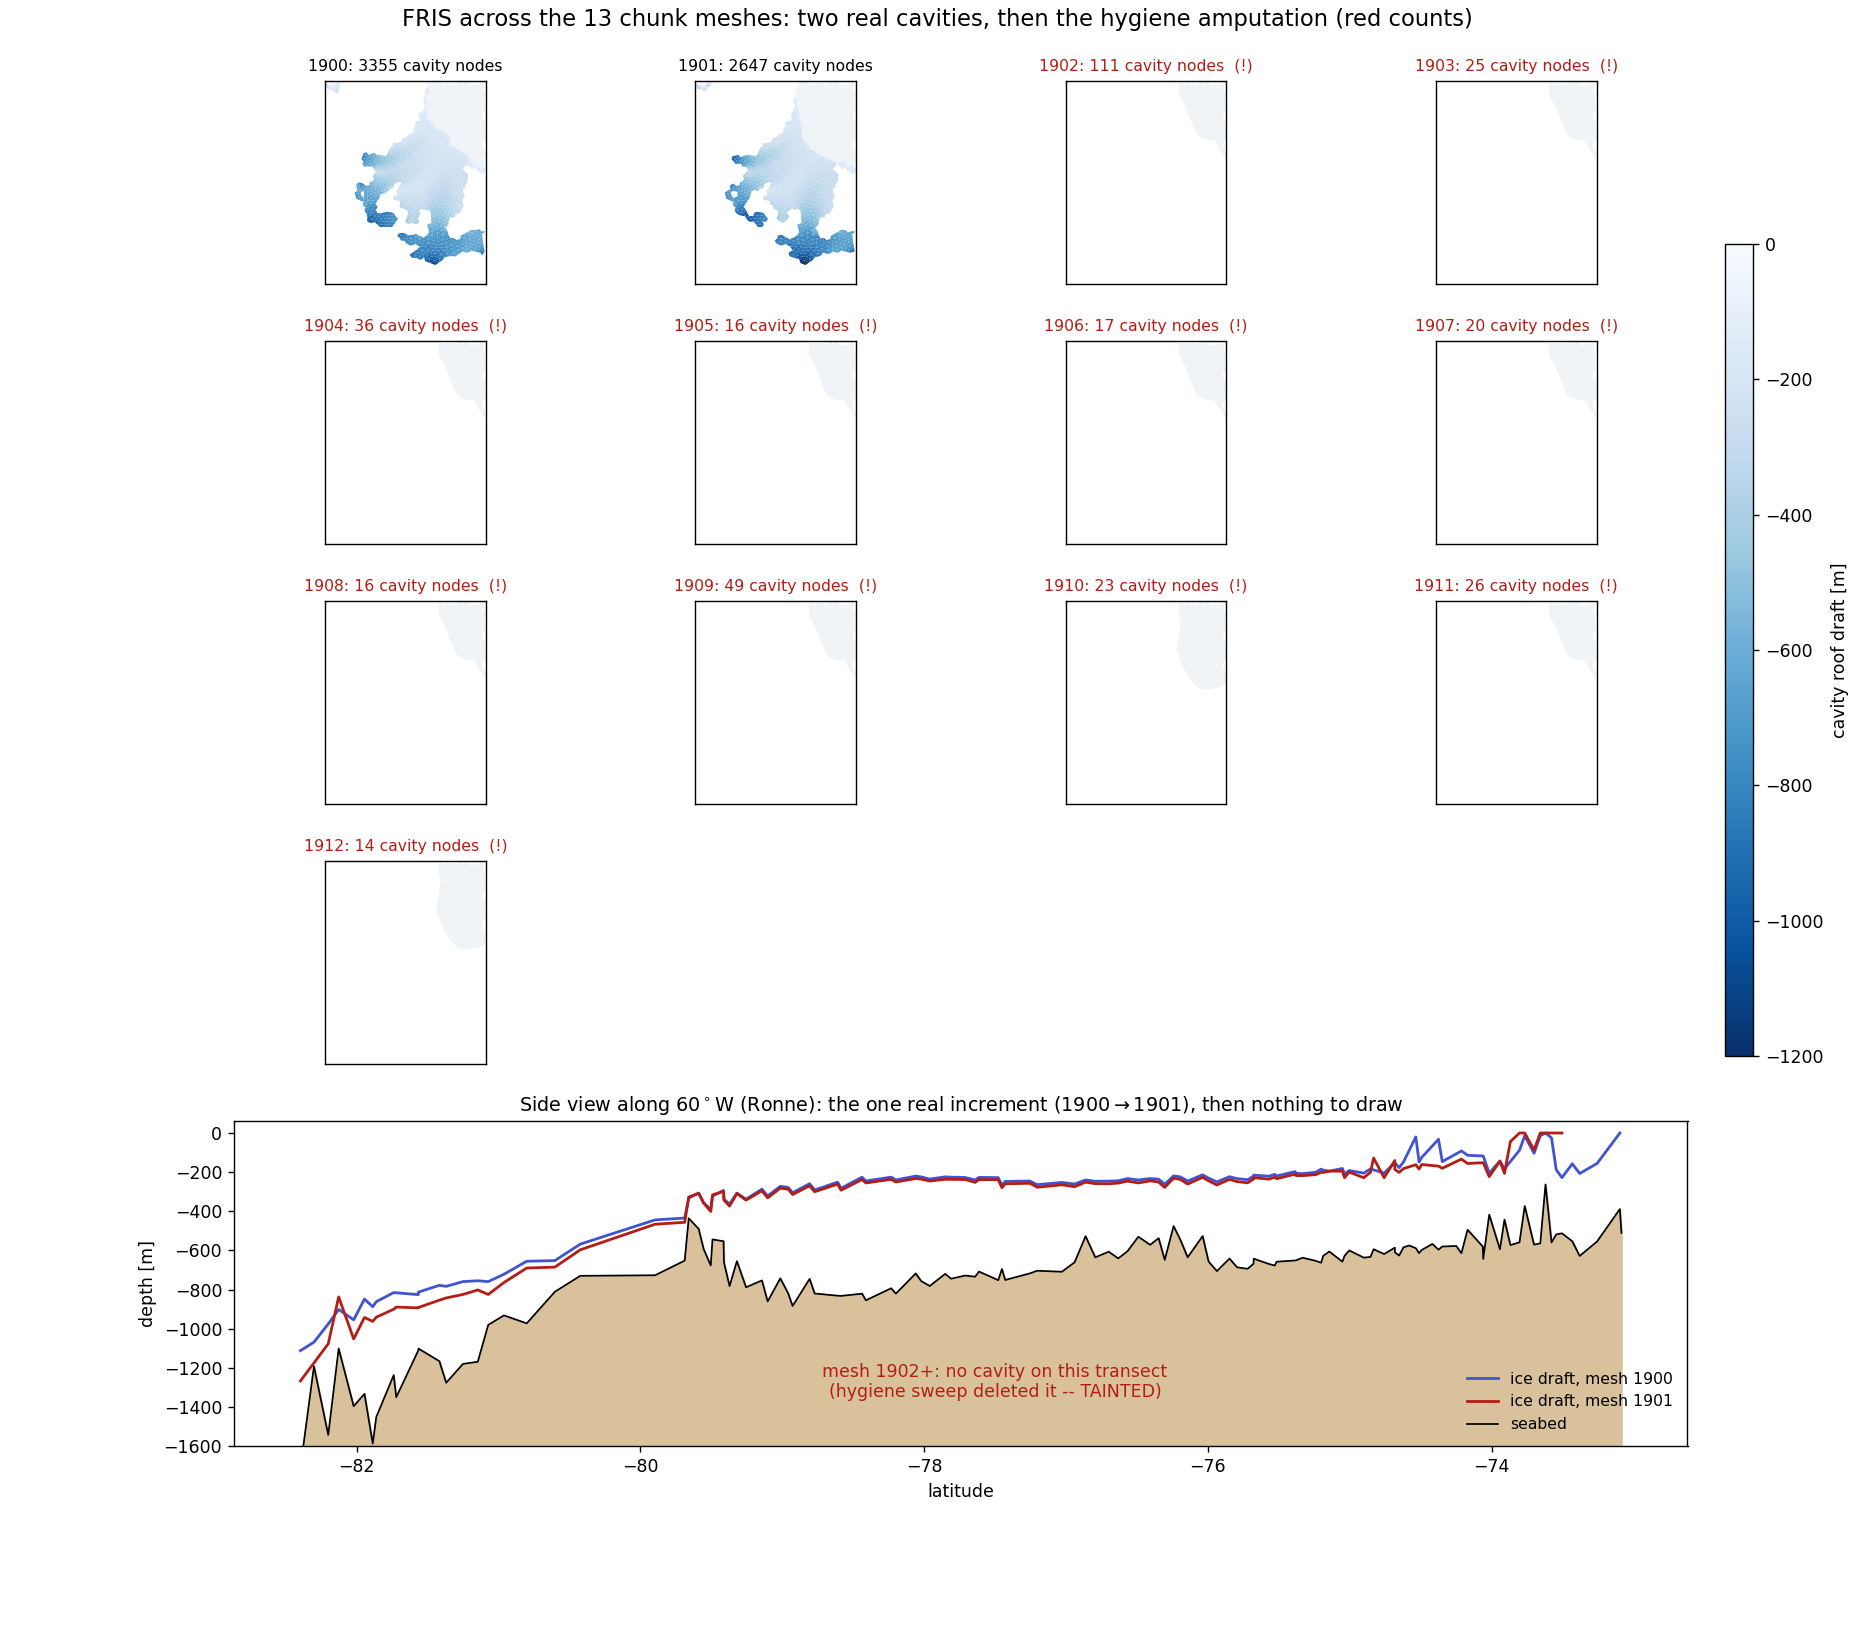
\includegraphics[width=\textwidth]{fris_top_side_chunks.png}
\caption{FRIS across the thirteen chunk meshes. Top grid: cavity elements coloured by roof
draft --- two real cavities (1900, 1901), then eleven empty frames with red node counts.
Bottom: ice draft along $60^{\circ}$W for the one genuine increment (1900$\to$1901; the
southern draft deepens by 50--100\,m), after which there is nothing left to draw.}
\label{fig:fris}
\end{figure}

\textbf{The problem to solve next} (Figs.~\ref{fig:evol}, \ref{fig:fris} are its
statement): make the mesh increments survivable \emph{without} destroying the cavities.
What is genuinely proven and stays: the full cycle
awiesm3\,$\to$\,PISM\,$\to$\,awiesm3-on-a-changed-mesh works end-to-end with real cavities
(movcav33 chunk-3 + handover; movcav34 chunks 1--4 reproduce it on the minimal build). The
work queue, in order: (i) a cavity-preserving fragile-sliver treatment --- removal must not
disconnect or cascade through the few-element-wide cavity bands (guard on the shelf flag, a
connectivity-preserving criterion, plus a safety valve that aborts the leg if the submesh
cavity count drops far below the classifier's flag count); (ii) rewind movcav34 to chunk-5
and re-run the increments with real cavities; (iii) the recurring OIFS \code{voskin}
coastal overflow; (iv) the iterative-coupling loop ignores \code{final\_date}; (v) the
escalating warm-bias melt that drives PISM's fast geometry increments in the first place.
Items (i) and (v) are worked below.

\subsection{The coastline is not the problem --- the increment is (2026-07-18)}\label{sec:hygiene}

The Ross-front blowup looked like a fragile coastline (24 nodes held by $\le3$ elements
within $1.5^\circ$ of the epicentre, including an 18-level cavity sliver on two triangles),
so the first response was a hygiene sweep removing ice-domain nodes held by $\le2$ elements.
It ran the chain to year 1911 --- but by \emph{amputating the cavities} (Bug ``VIII'',
above). An offline harness on the saved 1902 flag files then settled the question by
building submesh variants without submitting jobs:

\begin{itemize}
\item \textbf{Fragility is normal, not pathological.} The meshes that ran clean full years
  carry the \emph{same} fragile census as the crashed one: pool 3470 nodes with $\le2$
  elements (429 in cavities), submesh\_1901 3448 (378), versus 1902's 3444. A control that
  kills the hypothesis: if $\le2$-element slivers were fatal, 1901 would have died too.
\item \textbf{The increment is the violence.} Measured as per-node cavity-roof change against
  the previous submesh: increment 1 (pool$\to$1901) max $|\Delta\mathrm{draft}|$ 451\,m,
  mean 0.96\,m; increment 2 (1901$\to$1902) max \textbf{1196\,m}, mean \textbf{8.7\,m}
  --- $9\times$ the mean, opening 13 vertical levels at the epicentre in one decade beside a
  506-node grounding advance. This is downstream of item (v): the warm-bias melt escalates
  (cavity-mean 0.9$\to$5.5$\to$24\,m/yr), so each decade's geometry step is larger than the
  last.
\end{itemize}

\textbf{Fixes committed.} (a) A \emph{cavity-amputation abort guard}: if the reduced submesh
retains $<50\%$ of the classifier's flagged cavity nodes, the leg fails loudly instead of
running a formally-valid but cavity-less ocean (the tripwire that would have caught Bug VIII
in one couple\_in instead of eleven tainted chunks). (b) The PISM mask-value \code{0}
(\code{MASK\_ICE\_FREE\_BEDROCK}) is now classified \emph{land}: a second, independent
island-deletion path (bare bedrock defaulting to ocean) that would have re-drowned Elephant
Island once its nascent cap finishes melting. \textbf{Rejected:} a per-increment cavity-roof
\emph{rate limiter} (clamp the roof to within 75\,m of the previous leg). It worked offline
(retained 2221 cavity nodes vs 1864 unclamped) but was \emph{rejected on physics grounds}:
it makes the ocean's cavity geometry deliberately lag the ice sheet's, a coupler-imposed
inconsistency between components. The increment must be tamed at its source (the melt, next)
or by numerical treatment of the post-increment transient --- not by distorting the coupled
geometry.

\subsection{Why the cavity melt is high and rising, and how to slow it (2026-07-18)}\label{sec:melt2}

Item (v), the disease under the increments: the PI-control cavity melt runs at
$\sim$5.5\,m/yr area-averaged against an observed circum-Antarctic $\sim$0.8\,m/yr, and
\emph{escalates} (0.9$\to$5.5\,m/yr over 1900$\to$1901 on real cavities). Diagnosed from
the monthly \code{temp}/\code{salt}/\code{fw}/\code{unod}/\code{vnod} output
(Fig.~\ref{fig:melt}); the cause is not where the first pass guessed.

\begin{figure}[H]
\centering
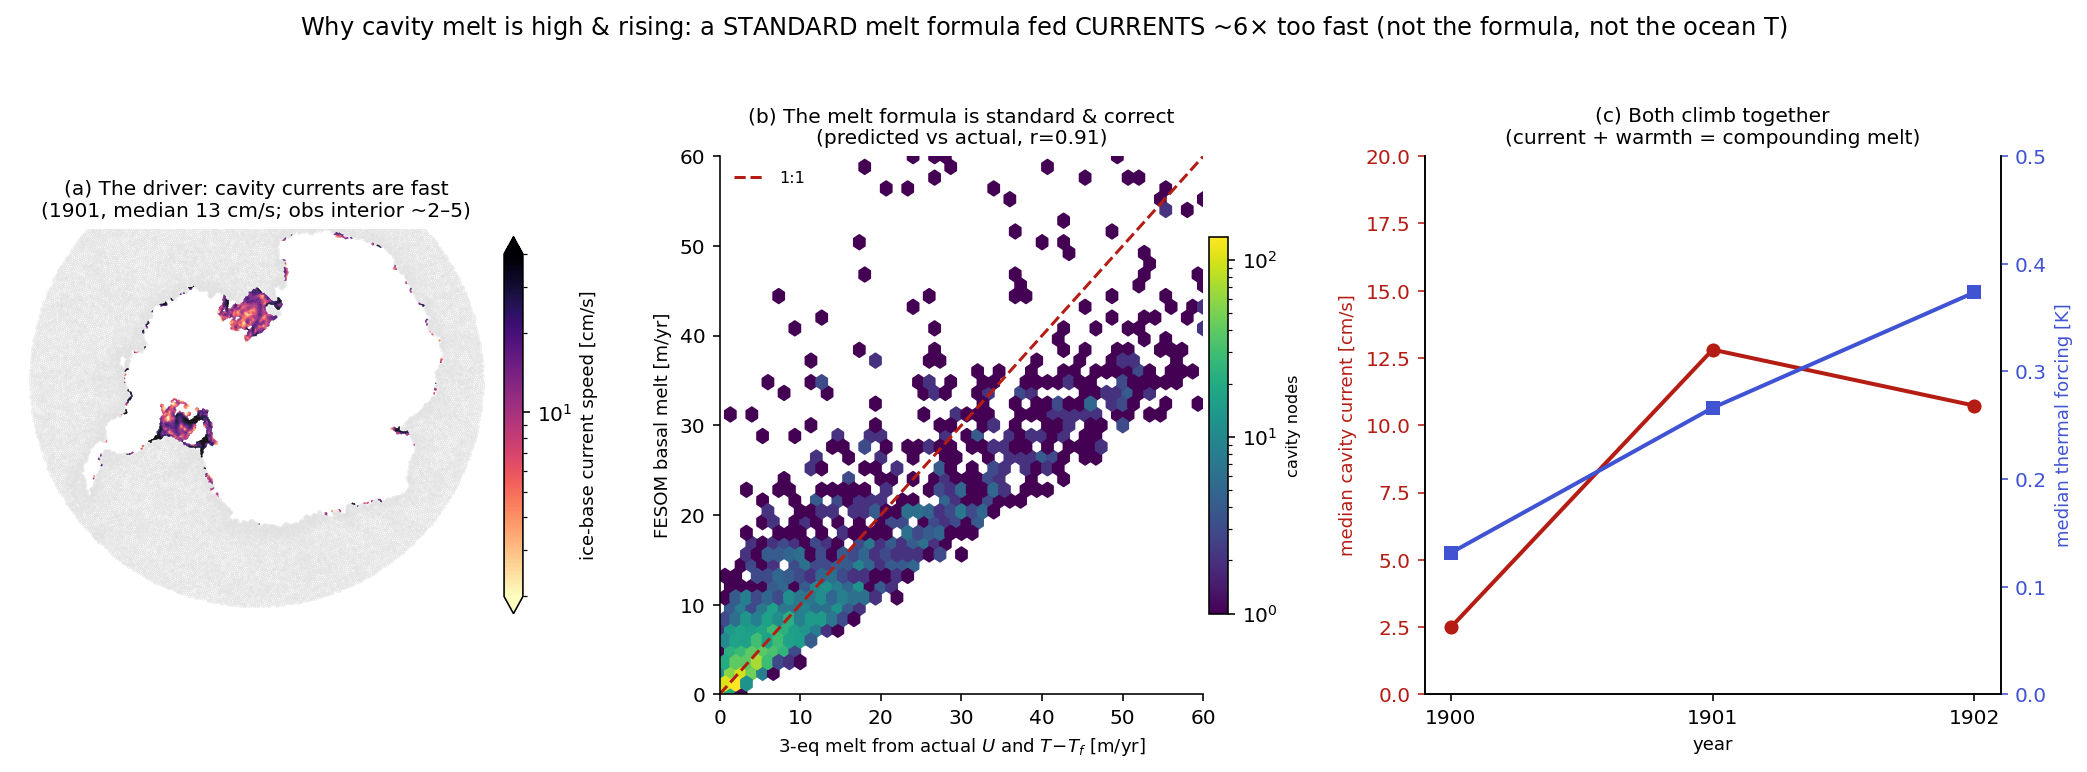
\includegraphics[width=\textwidth]{melt_diagnosis.png}
\caption{Why cavity melt is high and rising. (a) Cavity ice-base current speed (1901): median
13\,cm/s, mean 18, $61\%$ of nodes above 10\,cm/s --- fast, concentrated at the
Amundsen/Bellingshausen shelves and the Ross/Filchner ice fronts (observed cavity interiors
are a few cm/s). (b) The melt \emph{formula} is standard and correct: fed FESOM's actual
currents and thermal forcing, the three-equation scheme reproduces the model's own melt
(predicted vs actual $r=0.91$). (c) Both drivers climb together --- thermal forcing (median
$+0.13\to+0.37$\,K, warm-water intrusion) and current speed --- so the melt compounds.}
\label{fig:melt}
\end{figure}

\textbf{The chain, measured.} Thermal forcing $T-T_f$ at the ice-base level is
\emph{near-realistic} (area-weighted $+0.14$\,K; median $+0.13$ in 1900 rising to $+0.37$ in
1902). The Holland \& Jenkins three-equation scheme in \code{cavity\_param.F90} is standard
(drag $a_k=2.5\times10^{-3}$, $\gamma_T\approx10^{-4}$\,m/s), and fed the model's own currents
and thermal forcing it \emph{reproduces the melt} ($r=0.91$, 18 vs 16\,m/yr): the formula is
not miscalibrated. By elimination --- melt $7\times$ too high, formula validated, temperature
realistic --- the excess lives in the \textbf{cavity currents}: median 13\,cm/s where
$\sim$2\,cm/s would give the observed melt, i.e.\ $\sim6\times$ too fast. Because the
exchange velocity is $\gamma_T\propto|U|$, that fast circulation is exactly what inflates the
melt; and as the shelves thin the currents speed up further --- the escalation.

\textbf{How to slow it without killing the climate response.} The design constraint is to
dissipate \emph{momentum} with a flow-dependent operator, never to cap the diagnostic
(velocity, $\gamma_T$, or melt) --- a quadratic drag still lets the current find a slower
equilibrium that shifts with forcing, whereas a cap freezes the response. The ice base is
\emph{not} free-slip: \code{cavity\_momentum\_fluxes} already applies quadratic drag
$-\rho\,C_d|U|U$ at \code{nzmin}, correctly ordered (cavity elements skip the atmospheric-
stress overwrite, then receive the drag). But it borrows the \emph{seabed} coefficient
$C_d=2.5\times10^{-3}$ with the developer's own flag in the source (``\emph{need to check the
sensitivity to the drag coefficient}''). The plan: split it into a separate, tunable
\code{C\_d\_cavity} (default $=C_d$) and raise it --- physically justified, since ice-shelf
bases are hydraulically rougher than a flat seabed (basal crevasses, terraces, keels), and
dedicated cavity models treat ice-base drag as a distinct tunable $\gtrsim$ seabed. Being
quadratic it preserves the velocity's climate sensitivity. Complementary flow-dependent
levers if drag alone is insufficient: a vertical-viscosity floor in the cavity boundary
layer, or Smagorinsky horizontal viscosity in cavities. \emph{Not} to be done: raising the
global $C_d$ (over-brakes the open-ocean bottom boundary layer everywhere). Validation
target: melt toward $\sim$0.8\,m/yr \emph{while preserving} the spatial melt--forcing pattern
($r=0.81$) and the warm-Amundsen/cold-FRIS contrast --- brake the amplitude, not the
geography. Caveat: part of the $2.5\to13$\,cm/s jump over 1900$\to$1901 is plausibly spin-up
plus the increment shock, so retune against a settled multi-year state, not a transient.

\textbf{On bias correction} (a design question raised alongside): observation-anomaly
(``delta'') ocean forcing is standard for stand-alone ice-sheet runs, and even
cavity-resolving projections bias-correct their \emph{atmospheric} forcing (Naughten et
al.\ 2018 force FESOM with CMIP anomalies on an ERA-Interim climatology, control on
reanalysis) --- but it would not cure this run: the thermal forcing here is already
near-realistic, so correcting $T/S$ addresses a problem we mostly do not have. The excess is
in the \emph{circulation}, upstream of both the melt formula and the water it is fed.

\emph{Superseded (2026-07-19):} the ``too-fast currents'' diagnosis holds, but the proposed
cure --- a tunable ice-base drag \code{C\_d\_cavity} --- does not: the standalone dissection
below shows the fast currents are \emph{injected by the increment}, not an under-damped
equilibrium (chunk-1 and both year-long cold-start equilibria run $\sim$2.6\,cm/s at the
stock drag). See \S\ref{sec:standalone}; the drag plan is moved to Falsified.

\subsection{The spin-up is the remapped restart, not the water --- a standalone dissection (2026-07-19)}\label{sec:standalone}

To test the ``fast currents'' hypotheses cheaply, a \emph{standalone} FESOM harness
(\code{build\_sa}, submesh\_1901, 20-day runs, $\sim$2\,min each) with a cavity
median-column-speed metric. It reproduces the disease and then dissects it
(Fig.~\ref{fig:bifurcation}).

\begin{figure}[H]\centering
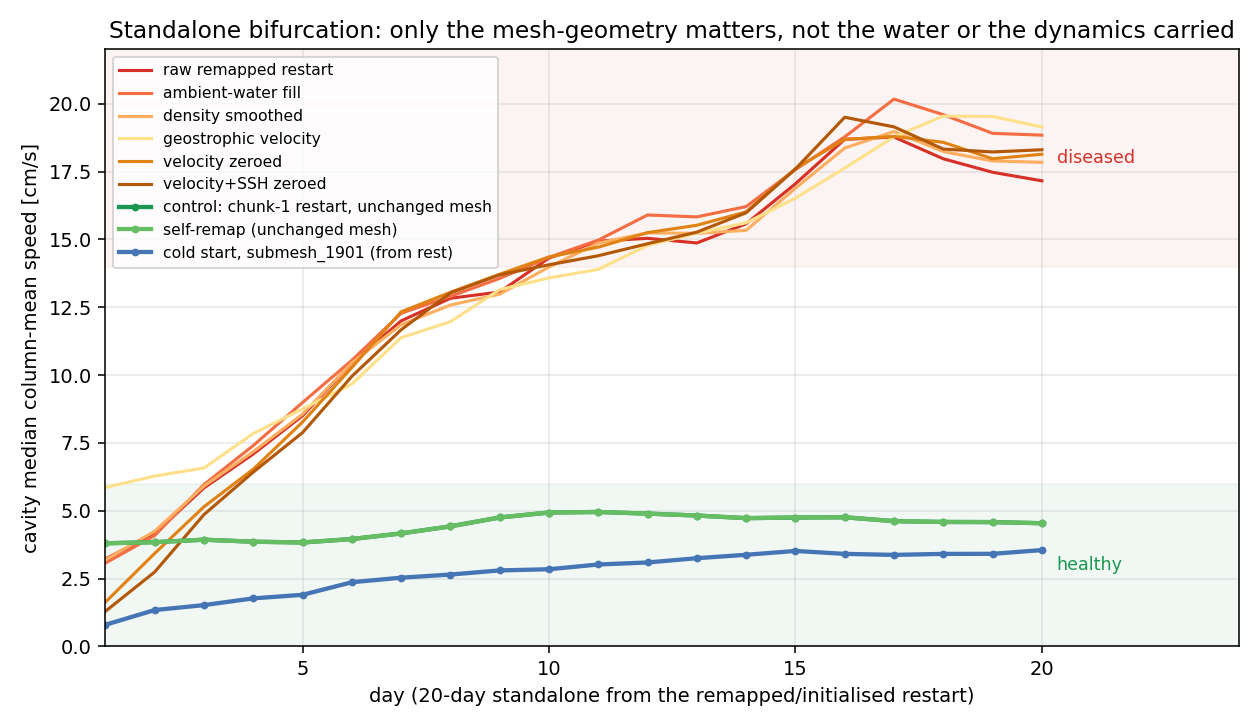
\includegraphics[width=\textwidth]{standalone_bifurcation.png}
\caption{Standalone cavity median speed vs.\ day. The runs bifurcate cleanly by \emph{what
mesh geometry} they use, not by the water or the dynamics carried. \textbf{Healthy
($\sim$2--5\,cm/s):} chunk-1 restart on the unchanged mesh (control), the same restart
remapped onto its \emph{own} mesh (self-remap, exonerating the remap machinery), and a
cold start from rest on the changed submesh\_1901. \textbf{Diseased (climb to
$\sim$17--19\,cm/s):} the raw remapped restart --- \emph{and} every attempted fix of the
carried state on that mesh: cavity density smoothed, cavity refilled with ambient
open-ocean water, geostrophic velocity imposed, velocity zeroed, velocity$+$SSH$+$hbar
zeroed. All fast, all indistinguishable. The excess is density-independent and not fixable
in any single carried field.}
\label{fig:bifurcation}
\end{figure}

\textbf{The elimination.} (i) The harness is faithful --- unchanged geometry stays slow,
through the remap or not. (ii) The cavity \emph{water mass is irrelevant}: chunk-1 water,
harmonically smoothed water and a fresh ambient reservoir all spin up identically ---
baroclinic/density is not the driver. (iii) The \emph{geometry is fine}: a cold start on
submesh\_1901 from rest settles to $\sim$2.6\,cm/s (1-year run, peaked $\sim$month~3 then
relaxed) --- a healthy equilibrium lives on the new mesh. (iv) It is not the individually
carried velocity, SSH or hbar (zeroing each $\to$ still fast) and \code{hnode} is already
nominal. \textbf{Conclusion:} the injector is the \emph{remapped restart being internally
inconsistent with the new mesh}; the geometry \emph{change} is only the trigger that exposes
it, not the cause.

\textbf{Footprint.} Matching submesh\_1901 to the initial submesh by coordinate: of 2627
cavity columns, \textbf{1602 changed vertical structure but the remap flags only 410}. The
classifier flags only columns that \emph{gain} wet levels (need fill: ice base shallower or
seabed deeper); the \textbf{1183 columns whose ice base got \emph{deeper}} (thicker ice
above $\to$ moved ice-loading/pressure boundary) are carried untouched. A density-independent,
geometry-linked lead --- not yet a proven cause.

\textbf{Learning the target (in flight).} Two 1-year cold starts with \emph{identical}
climatology and forcing, differing only in the mesh (1900 vs 1901), give two directly
comparable equilibria. Their difference $\Delta_{\mathrm{equil}}$ at the changed nodes is the
\emph{pure} ocean equilibrium response to the ice-draft change --- the first-principles
target a one-shot remap rule must reproduce (the old restart $\approx$ the 1900-mesh
equilibrium; the modification should push it to the 1901-mesh equilibrium, derived, not
copied).

\subsection{The seam field is \code{hnode} (2026-07-20)}\label{sec:hnode}

The equilibria then localised the seam to a single field. Building a rest state (velocity,
SSH, AB, hbar all zero) with the \emph{equilibrium} density and stepping it still spun up
(median 19\,cm/s) --- so density is finally, unconfoundedly dead. That rest state differs
from the healthy cold start in exactly one carried field: \code{hnode}, the ALE layer
thickness. Swapping the remap's \code{hnode} for the equilibrium's (the \emph{only} file
that changes, by $\le0.73$\,m) flips the cavity from 18.6 to 4.5\,cm/s, reproduced to two
digits (Fig.~\ref{fig:hnode}). The changed-column differences sit a couple of levels below
the moved ice base --- which is why every density/velocity/SSH test walked past it.
(\emph{Initially} read as ``differences entirely at the changed columns''; the correction
below shows the swap also moved the open-ocean \code{hnode}, which carries most of the effect.)

\begin{figure}[H]\centering
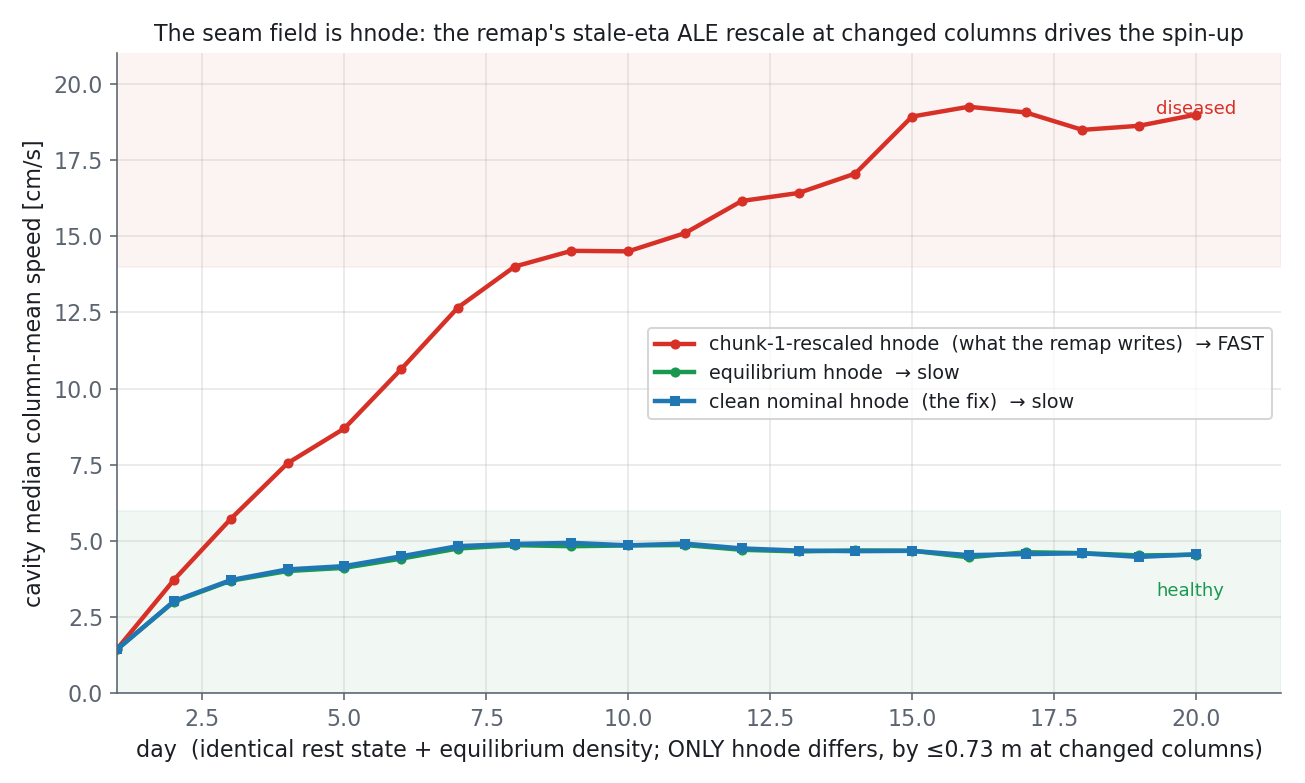
\includegraphics[width=0.82\textwidth]{hnode_seam.png}
\caption{One field, one flip. Identical rest state and equilibrium density; \emph{only}
\code{hnode} differs, by $\le0.73$\,m at the changed columns. The remap's chunk-1-rescaled
\code{hnode} (red) spins the cavity to $\sim$19\,cm/s; the equilibrium \code{hnode} (green)
and a \emph{clean nominal} \code{hnode} \emph{applied everywhere} (blue) both hold the
healthy $\sim$4.5\,cm/s. \emph{Caveat (added below):} this swap also changes the
\emph{open-ocean} \code{hnode}, not only the changed columns --- so it overstates what a
changed-column-only fix achieves (that reaches only $\sim$10\,cm/s).}
\label{fig:hnode}
\end{figure}

\textbf{Mechanism.} \code{remap\_hnode} rescales every changed column so
$\sum h = (z_{\mathrm{bar}}(ul)-z_{\mathrm{bar}}(nl)) + \eta_{\mathrm{new}}$, using the
\emph{remapped chunk-1} $\eta$. At changed columns that $\eta$ is stale --- starkest at
cavity$\to$open (``closed'') nodes, where it is the under-ice depressed value
($\approx-1.6$\,m) applied to a now-open column --- so the rescale \emph{compresses}
\code{hnode} (e.g.\ $10.0\to9.19$\,m). That inconsistent thickness is exactly the ``standing
$dh/dt$ source at $t{=}0$'' the rescale was added to prevent; it seeds the barotropic
spin-up. The rescale does the opposite of its intent because it trusts the carried $\eta$.

\textbf{Fix, and the correction (2026-07-20 late).} The \code{remap\_hnode} edit --- nominal
$z_{\mathrm{bar}}$ thicknesses at the geometry-changed columns (including the ice-base-deepened
ones the classifier calls ``unchanged'') instead of the stale-$\eta$ rescale --- was
implemented and regenerated end-to-end. In the standalone harness it \emph{halves} the
over-speed, $17\to10.3$\,cm/s: a real, physically-clean improvement, but \emph{not} a full
restoration. Reaching $\sim$4\,cm/s requires nominal \code{hnode} over the \emph{whole} ocean:
the fully-fixed and the target restarts turn out \emph{identical in the cavity} and differ only
in the \emph{open-ocean} \code{hnode}, and a cavity+ice-front-halo nominalisation does not help
(11\,cm/s) --- only nominalising everywhere does. So the earlier ``one field, one flip'' was
\emph{confounded}: the clean swap carried the open-ocean \code{hnode} too, not just the changed
columns. The residual is not the cavity fill but the \textbf{vertical-coordinate seam} at the
ice front --- zstar stretches the open-ocean layers by the free surface
($h_k = h_k^{\mathrm{nom}}(D+\eta)/D$) while the rigid-lid cavity keeps them nominal; the
remapped, zstar-stretched open-ocean \code{hnode} is what pushes the cavity from 4 to 10. This
reframes ``nominal everywhere'' not as a global-reset artifact but as precisely what
\textbf{\code{linfs}} (fixed layers, $\eta$ a top-boundary diagnostic) does by construction ---
removing the seam without any \code{hnode} surgery. \textbf{Confirmed}: the raw remap
(chunk-1 \code{hnode}, no surgery --- the exact restart that spins to 17\,cm/s under zstar) run
with \code{which\_ale='linfs'} does \emph{not} spin up; it decays to $\sim$1.7\,cm/s median /
2.5 mean and holds. So the seam, not the cavity fill, was the mechanism, and \code{linfs} is
the clean complete fix. Status: changed-column \code{remap\_hnode} fix implemented
(uncommitted, gives 10.3 --- now superseded by \code{linfs}); the open question is whether
\code{linfs} is acceptable model-wide for the coupled AWI-ESM3 open-ocean climate (a
linearised free surface with mass-conservation trade-offs vs.\ zstar).

\subsection{\code{linfs} in the coupled chain, and the open-cavity fill (2026-07-21)}\label{sec:linfs-coupled}

The standalone finding was then taken into the real iterative coupling: a fresh run
(\code{movcavlinfs}) with \code{which\_ale='linfs'} from chunk~1, everything else identical,
1200\,s timestep. It validates the seam story end-to-end (Fig.~\ref{fig:linfs-evo}). Four
mesh increments (1900--1903) hand over with \emph{no} cavity spin-up and \emph{no} CFL
blowup; the cavity node count is \emph{preserved} ($\sim$2668, vs the zstar run's collapse
$2647\to111$), the per-increment mesh change \emph{shrinks} as the ice-ocean system settles
($402\to187$ nodes added), and cavity melt is stable and realistic --- $\sim$0.22\,m\,w.e.\,yr$^{-1}$
cavity-mean, $\sim$1344\,Gt\,yr$^{-1}$ total (Rignot $\sim$1325), with none of the
$0.9\to5.5$\,m\,yr$^{-1}$ escalation seen under zstar. The vertical-coordinate seam was the
mechanism; \code{linfs} removes it in the coupled system too.

\begin{figure}[H]\centering
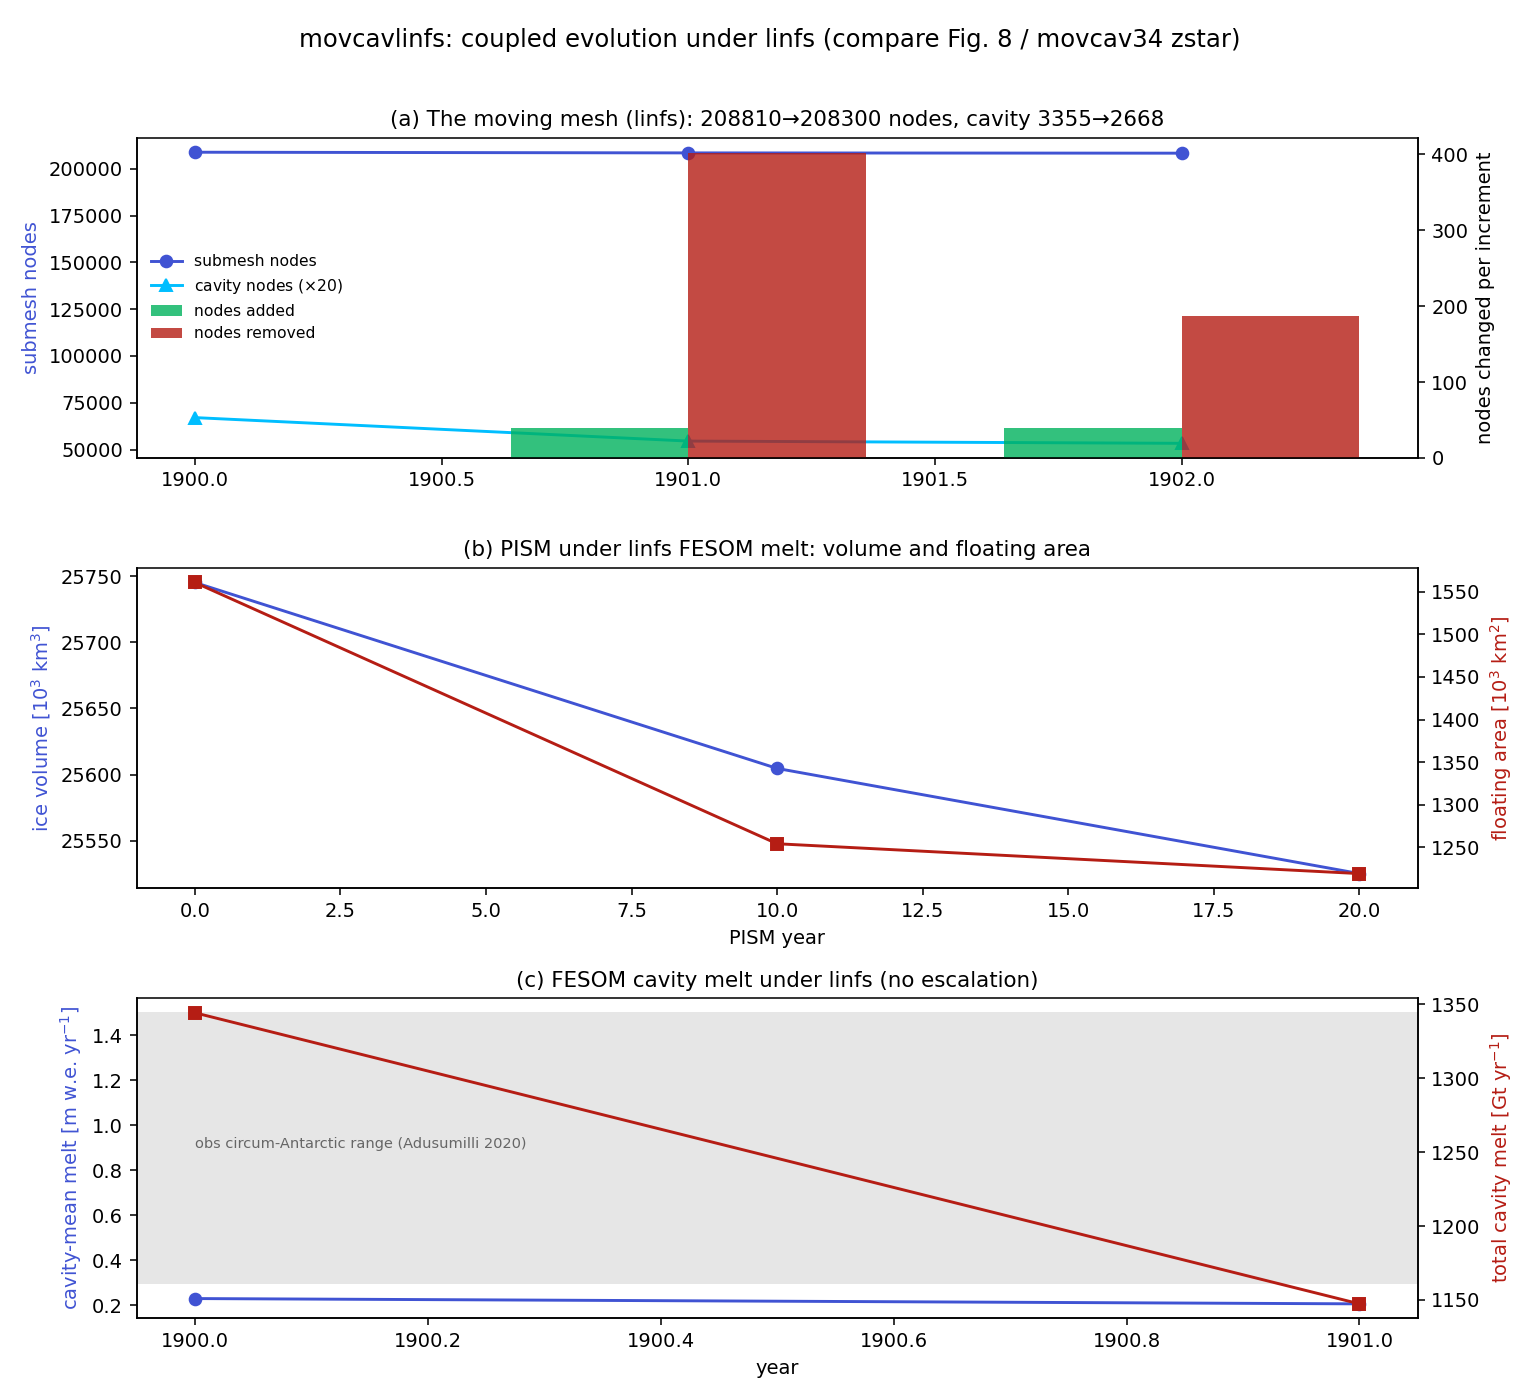
\includegraphics[width=0.92\textwidth]{movcavlinfs_evolution_timelines.png}
\caption{\code{movcavlinfs} coupled evolution under \code{linfs} (compare Fig.~8 / \code{movcav34}
zstar). (a) The moving mesh: node and cavity-node counts per increment, with nodes added/removed;
the increment shrinks and the cavity is preserved. (b) PISM ice volume and floating area. (c)
FESOM cavity-mean and total melt --- stable in the observed circum-Antarctic range, no escalation.}
\label{fig:linfs-evo}
\end{figure}

\textbf{The 1904 stop was a fill artifact, not the seam.} Chunk~5 (1904) tripped FESOM's fixed
temperature sanity reject (``\code{temperature becomes NaN or <-5.0}'') at step~1 on a cavity
node, $T=-5.35$. Not CFL, not spin-up. Two nested causes. (i) The remap carries each newly-iced
node's \emph{own open-ocean} column into the new cavity, so where the ice front advances over
warm water the ice base inherits it --- up to $+6.6$\,\textdegree{}C of thermal driving at the
new roof (Fig.~\ref{fig:newlyiced}a, red). (ii) A boundary-layer cap
(\code{cap\_new\_cavity\_temp}) that clipped those columns to the local freezing point
\emph{over-cooled} the deep part: at $\sim$4500\,m the pressure-depressed
$T_f = 0.0901 - 0.0575\,S - 7.61{\times}10^{-4}\,z \approx -5.35$\,\textdegree{}C, dragging real
$\sim-0.5$\,\textdegree{}C deep water below FESOM's $-5$ floor (Fig.~\ref{fig:newlyiced}a, blue).

\textbf{Fix: seed newly-iced columns from the nearest existing cavity} (user proposal). Instead
of carrying a node's open-ocean column (then capping it), each open$\to$cavity column is seeded
from the nearest column that is cavity in \emph{both} meshes, depth-matched. This gives cold,
cavity-appropriate ice-shelf water, regionally correct by nearest-neighbour (Amundsen-warm /
FRIS-cold preserved), with the deep column left real --- no cap needed. In the 1904 increment it
seeds 204 recipients from 2326 donors and cuts ice-base warm columns ($>0$\,\textdegree{}C) from
$61\to9$ and peak thermal driving from $+6.6\to+0.8$\,\textdegree{}C (Fig.~\ref{fig:newlyiced}, green
profile / right map); the residual nine are genuine warm East-Antarctic-coast cavities ($\le+0.8$).
A freezing-point floor (clamped to $-4.9$) is retained only as a last-resort backstop. No cap, no
crash, deep water preserved.

\begin{figure}[H]\centering
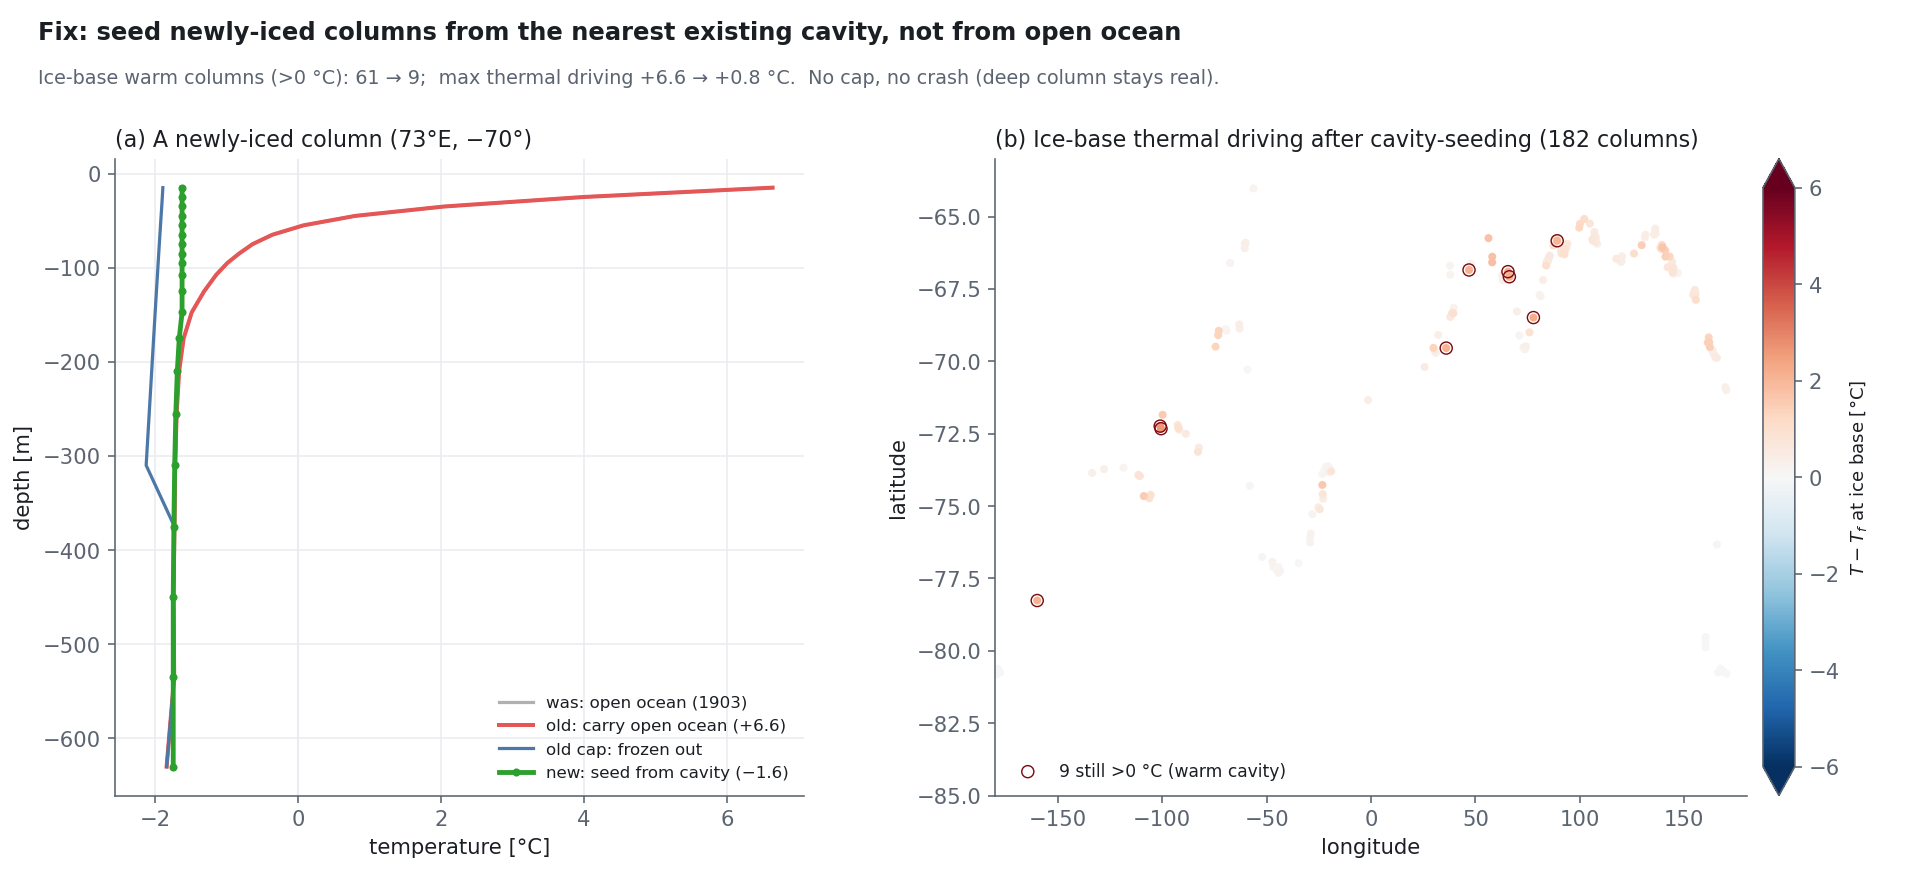
\includegraphics[width=0.98\textwidth]{newly_iced_warmwater.png}
\caption{The open-cavity fill fix. (a) A newly-iced column: carrying its open-ocean water (red)
puts $+6.6$\,\textdegree{}C at the ice base; the freezing cap (blue) over-cools the deep column;
seeding from the nearest existing cavity (green) gives a real cold ice-shelf-water profile with the
deep column intact. (b) Ice-base thermal driving $T-T_f$ over the 182 open$\to$cavity columns after
cavity-seeding --- almost all near freezing; the nine circled ($>0$\,\textdegree{}C) are physical
warm-cavity donors.}
\label{fig:newlyiced}
\end{figure}

\subsection{Case closed: the full \code{movcav37} cycle (2026-07-22)}\label{sec:movcav37}

With both fixes in place --- \code{linfs} (coordinate seam) and cavity-donor seeding
(open-cavity fill) --- a fresh run \code{movcav37} was launched from chunk~1 and carried the
complete decade 1900--1909: \textbf{ten coupled years, nine mesh increments, no spin-up, no
blowup} (it passes 1904, where \code{movcavlinfs} had stopped). This closes the spin-up
investigation.

The decisive metric is the cavity current itself (Fig.~\ref{fig:mc37speed}). The area-weighted
cavity median column-mean speed holds \textbf{1.1--2.1\,cm/s across all ten years} (p90
$\le5.2$), never leaving the healthy band --- against the 13--17\,cm/s the \emph{same} remapped
restart reached at every increment under zstar. The barotropic spin-up that this whole report
chased is, by construction, gone: it was the vertical-coordinate seam, and \code{linfs} removes it.

\begin{figure}[H]\centering
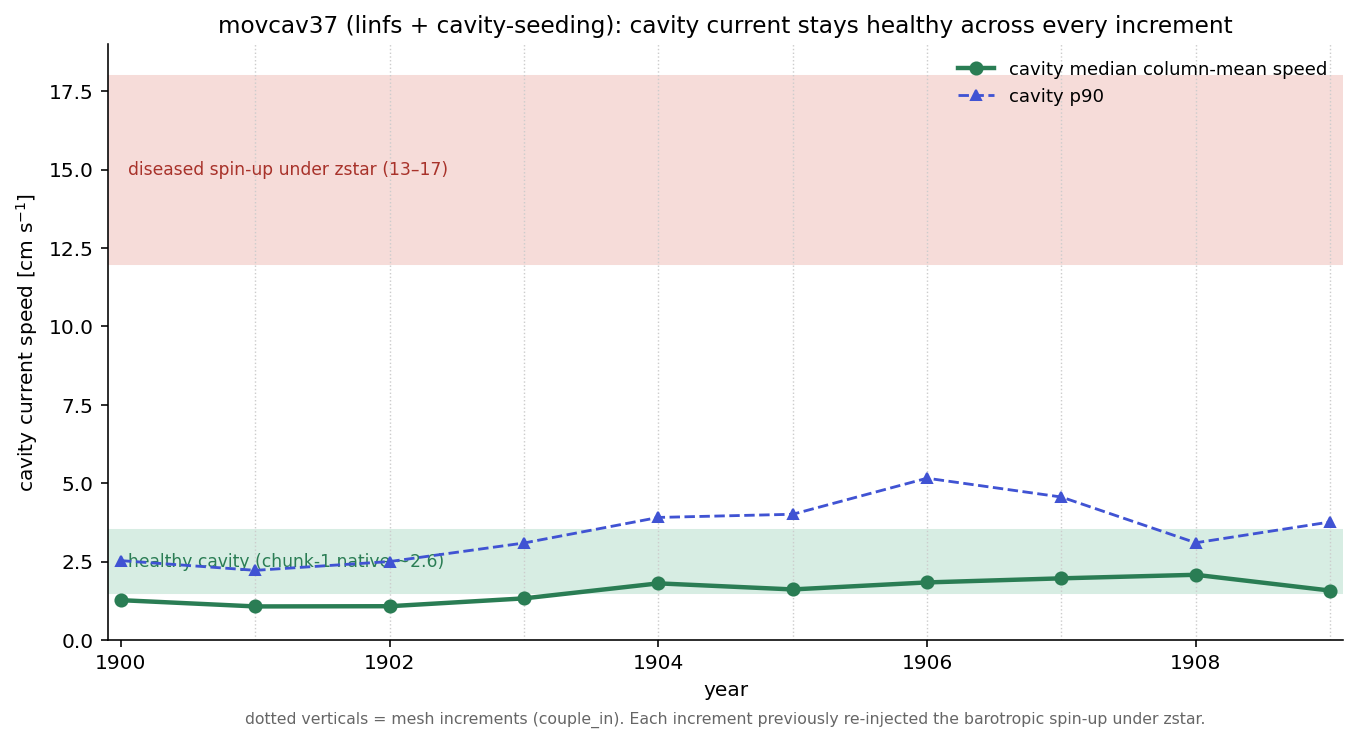
\includegraphics[width=0.9\textwidth]{movcav37_cavity_speed.png}
\caption{The spin-up, closed. \code{movcav37} cavity median (and p90) column-mean current speed
per year; dotted verticals are the nine mesh increments. The current stays in the healthy band
(chunk-1 native $\sim$2.6\,cm/s) at \emph{every} increment --- the 13--17\,cm/s diseased spin-up
under zstar (red band) never appears.}
\label{fig:mc37speed}
\end{figure}

The coupled system is also \emph{settling}, not diverging (Fig.~\ref{fig:mc37evo}). The cavity is
preserved (3355$\to$2318 nodes, a gentle thinning, not the zstar collapse to 111), the
per-increment mesh change shrinks ($405\to\sim$60 nodes), PISM volume and floating area decline
smoothly with no shocks at the increments, and cavity melt stays inside the observed
circum-Antarctic range (0.23$\to$0.82\,m\,w.e.\,yr$^{-1}$, 1329$\to$1685\,Gt\,yr$^{-1}$) --- no
trace of zstar's escalation to 5.5\,m\,yr$^{-1}$. The one feature to watch on a longer run is the
mild \emph{upward} melt trend; the flat 1--2\,cm/s currents identify it as thermodynamic/geometric
(shelves thinning, cavity warming slightly), not a dynamic spin-up, and it remains within observations.

\begin{figure}[H]\centering
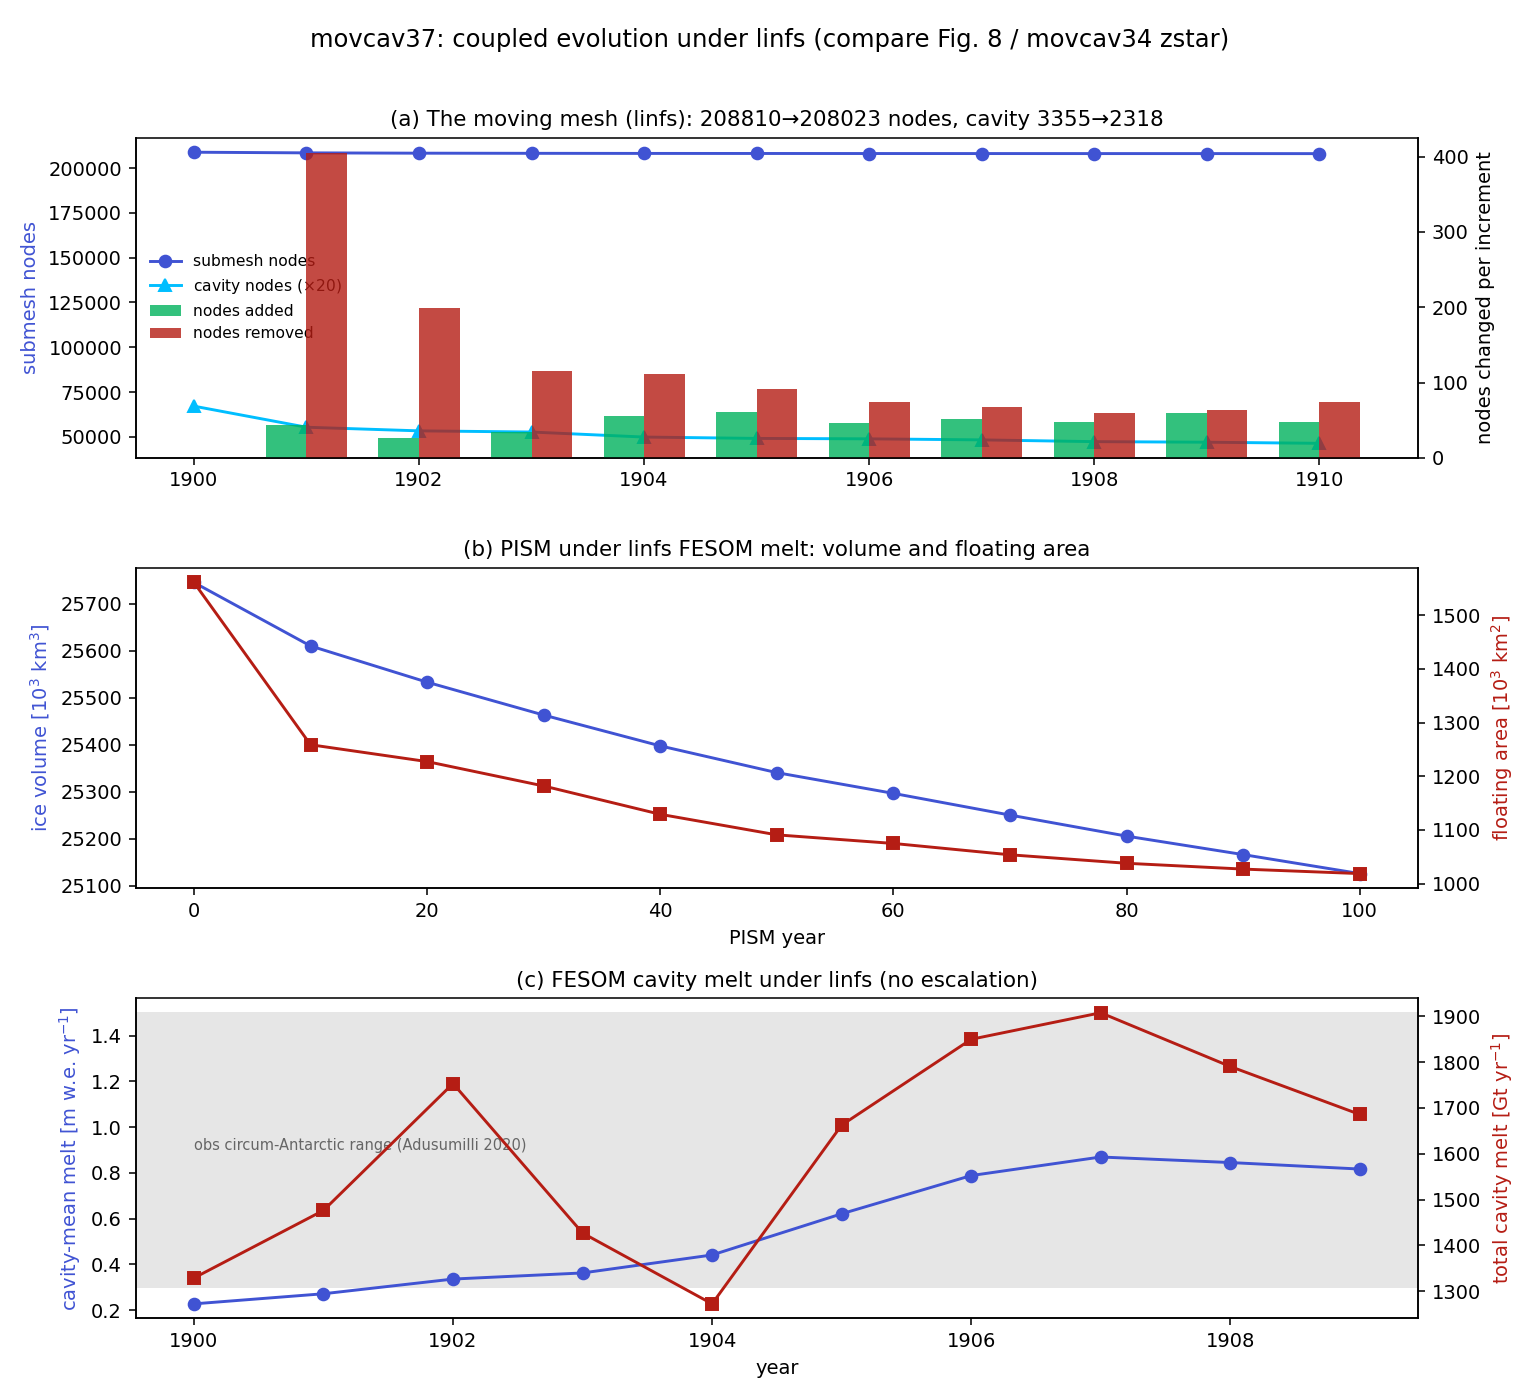
\includegraphics[width=0.95\textwidth]{movcav37_evolution_timelines.png}
\caption{\code{movcav37} coupled evolution (compare Fig.~\ref{fig:linfs-evo} / \code{movcavlinfs},
now the full decade). (a) Moving mesh: cavity preserved, increments shrink. (b) PISM volume and
floating area, smooth. (c) FESOM cavity melt, in the observed range, no escalation.}
\label{fig:mc37evo}
\end{figure}

\subsection{Sea ice and snow in \code{movcav37}: melt-back restored; the Ross lagoon (2026-07-22)}\label{sec:mc37seaice}

The open item of \S\ref{sec:seaicemelt} --- the SH summer melt-back and the coastal snow pile-up ---
is answered by \code{movcav37}. Diagnosed properly (sea ice lives on \emph{open-ocean} surface
nodes; cavity nodes carry spurious values and must be excluded), the thickness fields sit in the
observed range in both hemispheres (Figs.~\ref{fig:mc37seaice-ts},~\ref{fig:mc37seaice-maps}).

\begin{itemize}
\item \textbf{SH summer melt-back is restored.} The winter (Sep) pack is a coherent 0.4--1.0\,m ring
  (thicker in the Weddell/Ross gyres); by summer (Feb) it retreats almost completely to thin
  Weddell/coastal remnants --- the strong seasonal melt-back the reference had and the earlier movcav
  runs lacked. Hemispheric mean thickness $\sim$0.6\,m (obs ASPeCt/ICESat 0.5--1.0\,m).
\item \textbf{The coastal snow pile-up is gone.} SH snow is $<$0.15\,m over the pack with a coastal
  rim $\sim$0.25--0.35\,m, within the observed 0.1--0.4\,m --- not the 2--3.5\,m band of the pre-fix
  runs. (The \code{linfs} + clean chunk-1 ice init + coupled slab combination did restore the
  melt-back; this closes the \S\ref{sec:seaicemelt} question.)
\item \textbf{NH is realistic}: 2--4\,m ice against the CAA/Greenland thinning to the marginal seas
  (obs $\sim$1.5--3\,m), snow 0.15--0.35\,m in winter (Warren $\sim$0.2--0.4\,m).
\end{itemize}

\begin{figure}[H]\centering
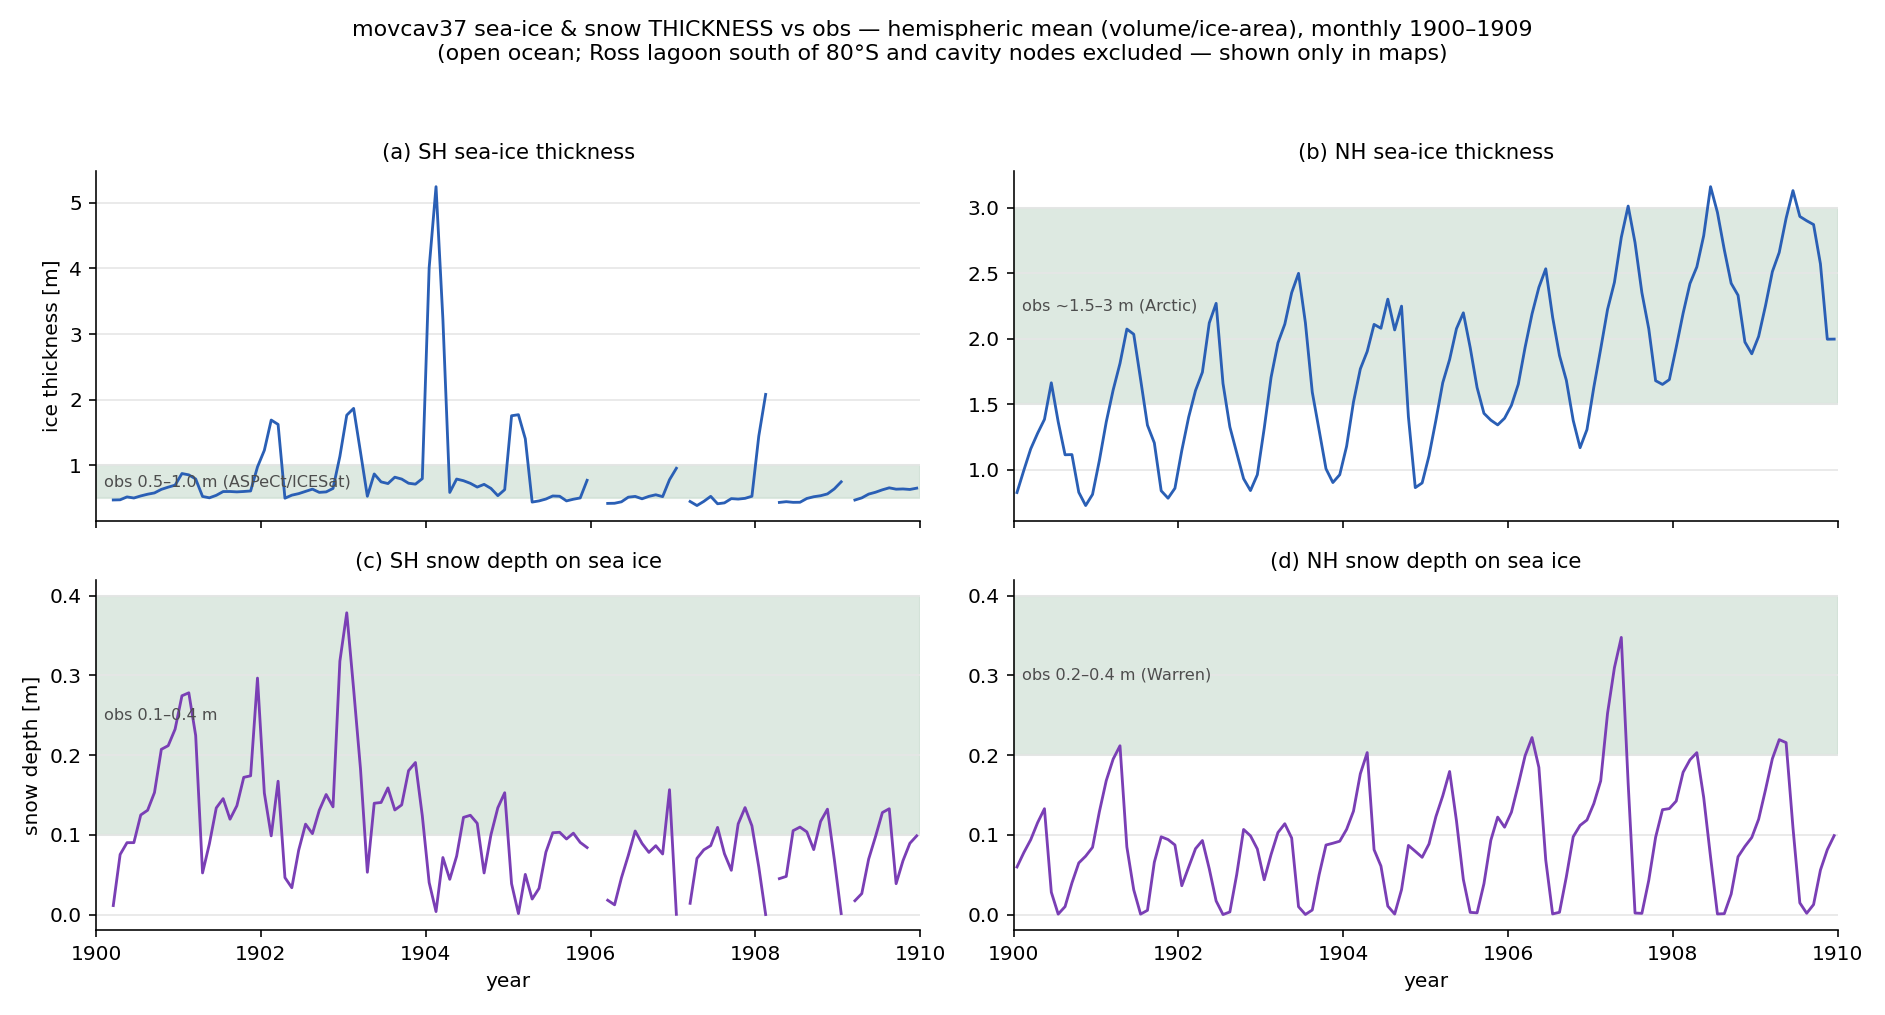
\includegraphics[width=0.98\textwidth]{seaice/movcav37_seaice_snow_thickness_ts.png}
\caption{\code{movcav37} sea-ice and snow thickness vs observations, monthly 1900--1909, hemispheric
mean (total volume / total ice-area over ice-covered open ocean, $a_\mathrm{ice}>0.15$). Green bands =
observed ranges. Cavity nodes and the Ross lagoon (open ocean south of 80$^\circ$S) are excluded here
and shown only in the maps. SH ice summer spikes are survivor bias (only thick coastal ice remains at
the Feb minimum).}
\label{fig:mc37seaice-ts}
\end{figure}

\begin{figure}[H]\centering
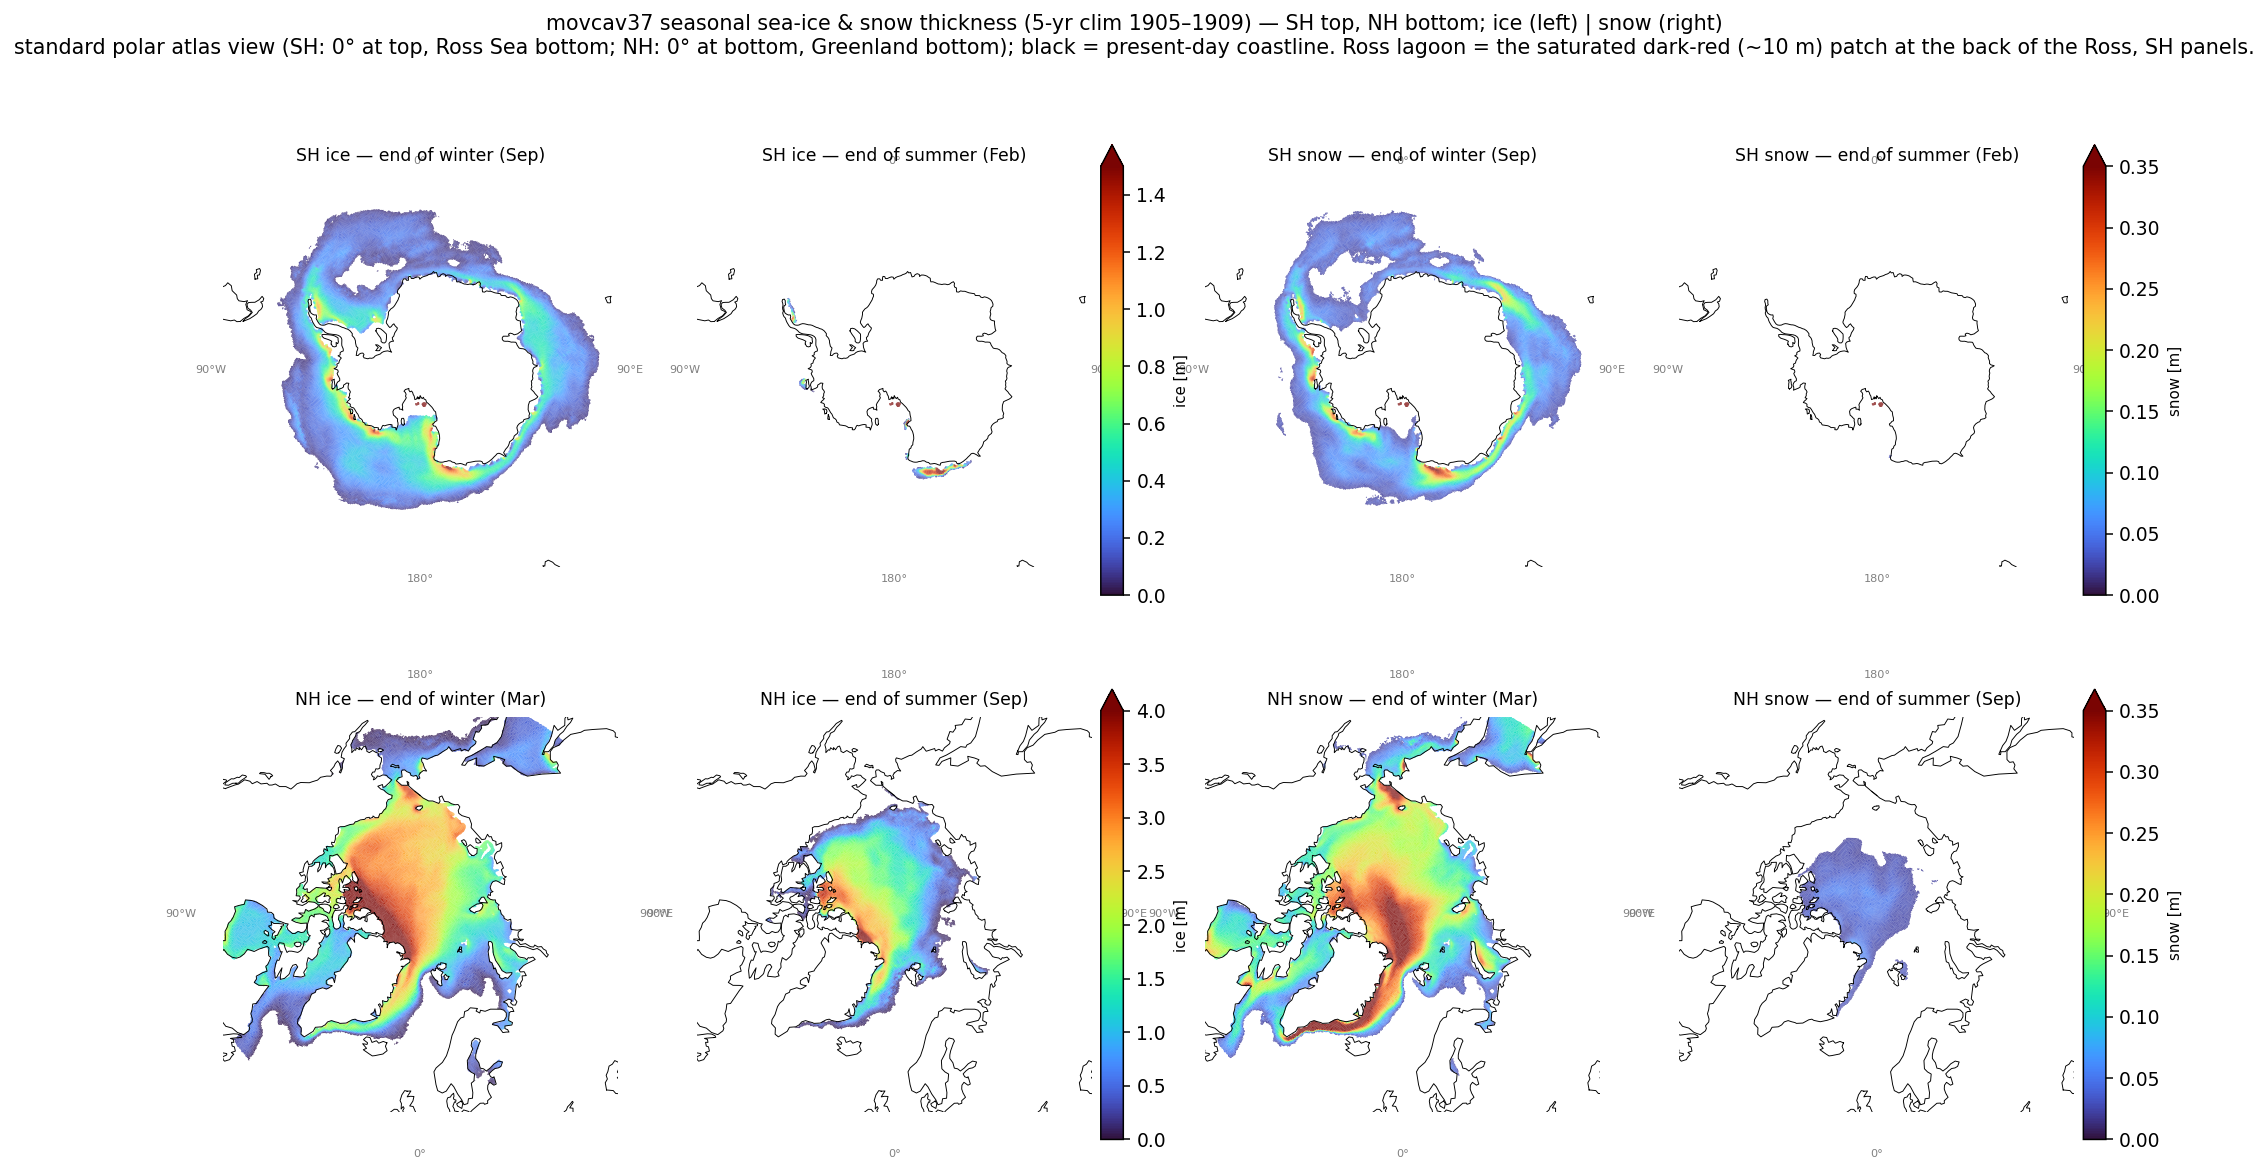
\includegraphics[width=\textwidth]{seaice/movcav37_seaice_snow_seasonal.png}
\caption{\code{movcav37} seasonal (end-of-winter / end-of-summer) sea-ice and snow thickness, 5-year
climatology 1905--1909, on the native grid (standard polar view, 0$^\circ$ meridian at bottom; grey =
present-day coastline). SH top, NH bottom; ice (left pair), snow (right pair). SH ice melts back to
near-nothing by February; SH snow is a thin coastal rim. The two dots off the Ross coast are the
\emph{Ross lagoon} artifact (below).}
\label{fig:mc37seaice-maps}
\end{figure}

\textbf{New open item --- the Ross lagoon.} The one unphysical thickness signal left is a small
($\sim$18-node) patch at the back of the Ross Ice Shelf (lon\,$\approx$\,180$^\circ$,
lat\,$\approx$\,$-83^\circ$) where PISM, over the run, thinned the shelf and retreated the grounding
line until the classifier flipped those nodes from \emph{cavity}/\emph{grounded} to \emph{open ocean}
(verified node-by-node: \code{cavity(ul=12--16)} or land in 1900 $\to$ \code{ul=1} by 1909). FESOM then
traps thick ($\sim$10\,m), convergent, non-melting sea ice in the near-enclosed deep embayment --- the
dots in Fig.~\ref{fig:mc37seaice-maps}. It is a PISM-geometry artifact (likely over-thinning the back
of the Ross, fed by excess FESOM cavity melt there), not a sea-ice-model problem; it is excluded from
the aggregates above. Fix candidates: guard the classifier against ungrounding interior nodes far
behind the shelf front, or address the excess back-of-Ross melt.

\subsection{The coupled-slab switch was off for \code{develop}/\code{develop-cc}; the sea-ice climate validated on a clean decade (2026-07-23$\to$27)}\label{sec:nammcc}

Rolling the coupled-slab work out from \code{develop-is} to the sibling setups \code{develop} and
\code{develop-cc} exposed a silent, months-old configuration bug. The coupled slab is
\emph{hardwired in the FESOM build} (\S\ref{sec:slab}: \code{ice\_thermo\_cpl.F90} sets
$Q_\mathrm{atmice}=-a2ihf$, so the atmosphere owns the ice-surface temperature and its slab
conduction must be fed the coupled ice thickness). OIFS is told to match through
\code{NAMMCC}: \code{LNEMOLIMTHK=.true.} (use the coupled thickness in the surface solve) and
\code{LNEMOLIMTEMP=.false.} (do not overwrite the ice skin from the ocean model each hour). The
OIFS defaults (\code{sumcc.F90}) leave \emph{both} \code{.false.}. Only \code{develop-is} set
\code{NAMMCC} --- and only because its \emph{runscript} did, by hand. So \code{develop} and
\code{develop-cc} silently ran with \code{LNEMOLIMTHK=.false.}: the \code{sit\_feom}$\to$%
\code{A\_Ice\_thickness} field added by the whole coupled-slab rollout was delivered over OASIS
and then \emph{discarded}, and the atmosphere conducted through a default slab thickness.

The signature was unmistakable once a clean 10-year \code{develop} run (\code{si10y}, TCO95--CORE3,
1990 GHG, fixed full mesh, no cavity) was diagnosed: with the switch off, the Arctic went
\emph{completely ice-free every June--October} and the winter pack carried half its proper volume
(NH March volume $5.3$; \S\ref{sec:state}). Setting the three \code{NAMMCC} switches turned that
into a physical sea-ice climate at the first attempt (Fig.~\ref{fig:si10y-maps}): NH March volume
$5.3\to27.4\times10^3$\,km$^3$ (obs $\sim$28--30), NH September extent $0.0\to5.6\times10^6$\,km$^2$,
SH February extent $0.0\to1.7$. The fix now lives in the setup config, not the runscripts
(\code{awiesm3.yaml}, commit \code{0aca2487}), applied to all three \code{develop*} versions;
tags keep the stock defaults because their component versions predate \code{sit\_feom}.

\emph{This does not taint the \code{movcav} results.} The \code{develop-is} runscripts set
\code{NAMMCC} by hand throughout, so every \code{movcav} run in this report (\S\ref{sec:slab}
onward) already had \code{LNEMOLIMTHK=.true.}. The bug lived only in the fixed-mesh siblings.

\begin{figure}[H]\centering
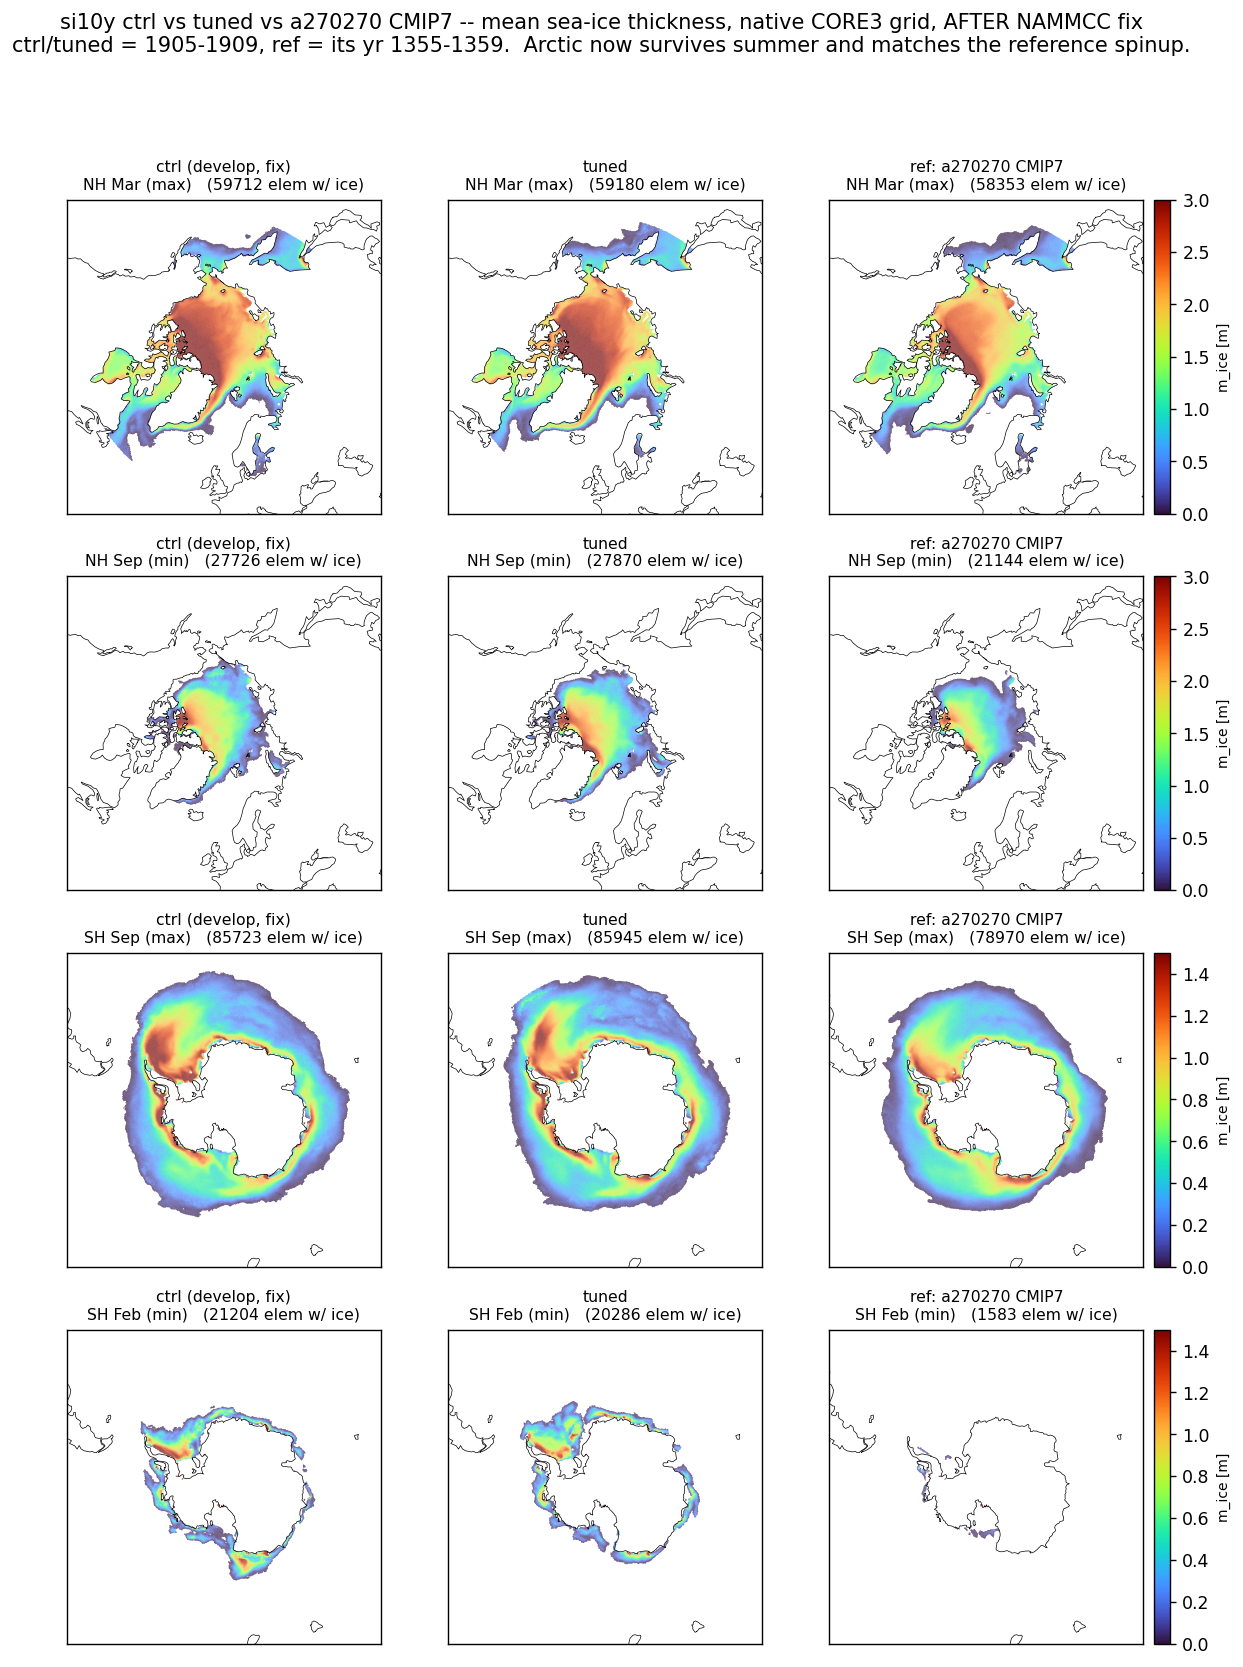
\includegraphics[width=\textwidth]{seaice/si10y_maps.png}
\caption{\code{develop} sea-ice thickness after the \code{NAMMCC} coupled-slab fix, native CORE3
grid, 5-yr mean of spin-up years 6--10, zoomed to the polar caps. Columns: control (fixed
\code{develop}), the tuning experiment (\S\ref{sec:state}), and an independent 500-year CMIP7
pre-industrial spin-up (a270270) at the same spin-up age. Rows: NH March (max), NH September (min),
SH September (max), SH February (min); element counts with $a_\mathrm{ice}>0.15$ annotated. The NH
September row --- blank (``NO ICE'') before the fix --- now carries a coherent central Arctic pack
\emph{exceeding} the reference (27.7k vs 21.1k elements). The large-scale fields match the reference
spin-up hemisphere-by-hemisphere; the coupled-slab config is correct.}
\label{fig:si10y-maps}
\end{figure}

Quantitatively, against 1990s observations and the a270270 pre-industrial spin-up sampled at the
\emph{same} spin-up age (years 6--10 of each), last-5-year means:

\begin{center}\small
\begin{tabular}{@{}lccl@{}}
\toprule
metric & \code{develop}+fix (1990) & a270270 (PI) & obs \\
\midrule
NH March extent [$10^6$\,km$^2$]     & 16.1 & 15.4 & $\sim$15.5 (NSIDC 1990s) \\
NH September extent [$10^6$\,km$^2$] &  5.6 &  4.7 & $\sim$7.0 \\
NH March volume [$10^3$\,km$^3$]     & 27.1 & 23.1 & $\sim$28--30 (PIOMAS) \\
NH March mean thickness [m]          & 1.8  & 1.6  & $\sim$2.3--2.6 \\
SH September extent [$10^6$\,km$^2$] & 21.4 & 20.3 & $\sim$18.5 (NSIDC) \\
SH February extent [$10^6$\,km$^2$]  &  1.7 &  0.0 & $\sim$3.0 \\
SH September mean thickness [m]      & 0.7  & 0.6  & $\sim$0.9--1.2 \\
\bottomrule
\end{tabular}
\end{center}

The fixed run is closer to observations than the reference on every row (Fig.~\ref{fig:si10y-vs-ref}).
Two residual biases remain, both ordinary sea-ice tuning territory and neither addressed by the
\code{whichEVP}/melt-pond tuning that was tried (it moved nothing): \textbf{NH ice is $\sim$20--25\%
too thin} (thin pack, under-done September minimum), and \textbf{the SH seasonal cycle is too
extreme} (over-grows in winter, over-melts in summer). A single-point thickness runaway
($\sim$52\,m at year 10) is present \emph{identically in the reference} (which reaches 855\,m by its
year 500): a shared FESOM point-convergence artifact, not introduced by the coupling.

\begin{figure}[H]\centering
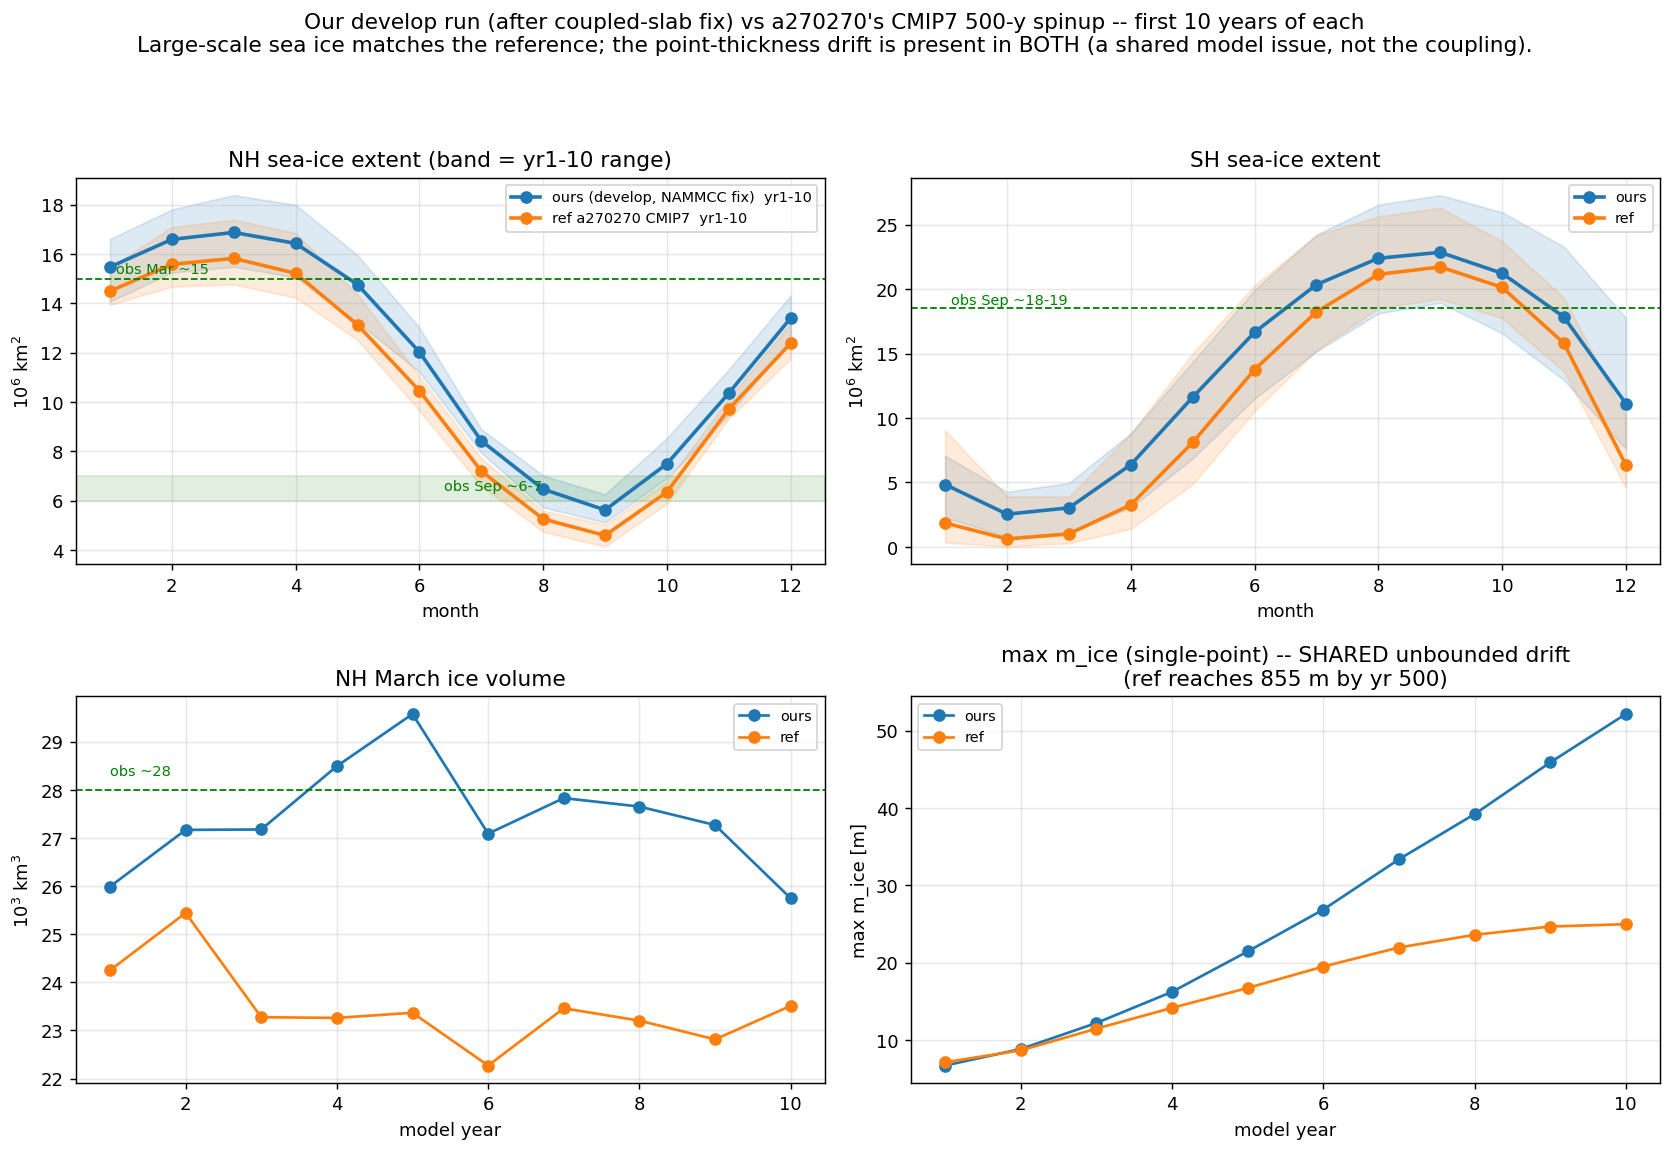
\includegraphics[width=0.92\textwidth]{seaice/si10y_vs_ref.png}
\caption{\code{develop}+fix (blue) vs a270270's CMIP7 pre-industrial spin-up (orange), first 10
years of each. (a,b) NH/SH seasonal extent, band = year-range; green markers = observed. (c) NH
March volume; (d) single-point max thickness --- the unbounded drift is present in \emph{both} runs
(shared model artifact). Large-scale sea ice matches the reference; where the two differ, the fixed
run sits closer to observations.}
\label{fig:si10y-vs-ref}
\end{figure}

A throughput trap surfaced while setting these runs up, worth recording because no short test
catches it: with \code{oasis3mct.lresume=false} the coupling restart is rebuilt every exchange and
the step rate decays $\sim$100$\times$ over a run ($0.28\to11.4$\,s/step); \code{lresume=true} (from
a matching restart set carrying \code{sit\_feom}) holds it flat at $\sim$0.10\,s/step. See Method
notes.

\subsection{The \code{voskin:282} overflow, inventoried across the campaign and instrumented (2026-07-24)}\label{sec:voskin-inventory}

The WAM fix (\S\ref{sec:wam}) closed one route into \code{voskin\_mod.F90:282}, but the line kept
killing later legs. Sweeping every \code{error (72)} floating overflow in the \code{develop-is}
history gives eleven crashes, all on OIFS ranks and only ever at the rank extremes (OpenIFS
decomposes north$\to$south, so the extremes are the poles --- never the mid-latitude ranks):

\begin{center}\small
\begin{tabular}{@{}llll@{}}
\toprule
run(s) & chunk & hemisphere & crash site \\
\midrule
movcav18/24/26/28/30/31 & 1 (1900) & both poles & \code{cubasen:453}, \code{vsurf\_mod:280} \\
movcav19                & 5 (1904) & Arctic     & \code{cubasen:453} \\
movcav33                & 2 (1901) & Antarctic  & \code{callpar:678} \\
movcav34                & 13 (1912)& Antarctic  & \code{voskin\_mod:282} \\
movcav39                & 2 (1901) & Antarctic  & \code{voskin\_mod:282} \\
par03                   & 2 (1901) & Antarctic  & \code{voskin\_mod:282} \\
\bottomrule
\end{tabular}
\end{center}

Two families separate cleanly by chunk. \textbf{Chunk~1} crashes (\code{cubasen}/\code{vsurf}, both
poles) are the pinned-skin sea-ice-thermodynamics instability, Bug~IV --- gone under the coupled
slab. \textbf{Chunk~$\ge2$} crashes (\code{voskin}/\code{callpar}, \emph{Antarctic only}) are the
mesh-increment family, and they persist.

\code{voskin:282} is the \emph{detector, not the cause}. The build is single precision
(\code{libsurf.SP.so}, max $\sim$$3.4\times10^{38}$); line 282 is the Langmuir number
$Z_\mathrm{LA}=[\rho_a/\rho_w\cdot Z_\mathrm{UST}^2 / \max(u_\mathrm{St}^2{+}v_\mathrm{St}^2,10^{-8})]^{1/4}$,
whose argument is $\sim$$1.2\times10^5\cdot Z_\mathrm{UST}^2$ --- it overflows only once the friction
velocity $Z_\mathrm{UST}$ already exceeds $\sim$$5\times10^{12}$. Upstream (lines 193--204)
$Z_\mathrm{UST}$ is built from the surface stress \code{PUSTR/PVSTR} and a buoyancy amplifier
$Z_\mathrm{WST2}/Z_\mathrm{DU2}$ that divides by the skin temperature \code{PTSKM1M}; it is floored
by \code{ZEPUST} but \emph{never capped}. For par03 the crashing leg's inputs were all checked and
clean: the seven A096 fields of \code{rstos.nc} (including \code{A\_CurX/Y}, which set the
wind-relative-to-current stress) all physical, the regenerated ICMGG \code{skt}/\code{sst}/\code{ci}
physical, and the \code{A\_SST} coastline sanitizer (\S\ref{sec:bug3} lineage, commit
\code{e5d4796c}) \emph{ran} on that leg yet the crash still occurred. So the bad value is
\emph{generated inside the first timestep}, which is why file inspection has not found it.

Two diagnostic probes were added to \code{voskin\_mod.F90} (dump the column inputs when
$Z_\mathrm{UST}>10$ or non-finite, and when the buoyancy $Z_\mathrm{BUO}$ blows up or
\code{PTSKM1M}$<100$\,K), OIFS rebuilt (\code{develop-is}; \code{VOSKIN-DIAG} strings verified in
\code{libsurf.SP.so}). The instrumented reproduction --- par03 chunk~2 crashes $\sim$60\,s in ---
is \textbf{ready but not yet run} (it mutates the par03 experiment). Its output will separate the
two candidate routes: huge \code{PUSTR/PVSTR} (stress arrived broken from the turbulence scheme)
vs.\ a collapsed \code{PTSKM1M}/large fluxes (the buoyancy amplifier). \emph{This is the current
open front for the mesh-increment crash family.}

\subsection{Two more crash faces: a mid-year FESOM flux blow-up and a leg-start numerical explosion (2026-07-30)}\label{sec:2026-07-30}

The \code{voskin:282} front (\S\ref{sec:voskin-inventory}) is OIFS-side and fires on step~1. Two
\emph{new} crash faces surfaced this week, both on the \emph{FESOM} side, and neither is
\code{voskin:282}.

\textbf{(i) A mid-year FESOM flux blow-up.} A colleague's 17-cycle concurrent run
(\code{repro\_movcav45}) died in FESOM's own \code{check\_blowup}, not OIFS: cycle~19 (1918),
\code{mstep}~14458 (mid-year, $\sim$day~201), at an \emph{Arctic} node (lat~$+83.5^\circ$,
lon~$-53^\circ$). \code{temp} hit $227^\circ$C, driven by a garbage surface heat flux
\code{hflux}$=-4.0\times10^{6}$\,W/m$^2$ ($\sim$$10^4\times$ any physical air--sea flux) at an
ice-edge node where sea ice vanished in a single step (\code{m\_ice} $1.27\to0$). Only the surface
layer blew up (every layer below normal, $-1.4\ldots-0.4^\circ$C) and CFL stayed $<1$ throughout, so
this is a \emph{surface-flux injection}, not an interior/velocity instability. The submesh the coupler
built for that leg was \emph{clean} --- cavity front stable at $\sim$704\,km every year (1910--13),
matching PISM's $\sim$690\,km --- so the PISM$\to$FESOM geometry conversion
(\code{mesh\_flags.py}\,+\,\code{fesom\_submesh.x}) is \emph{correct}; the bad flux is delivered by the
atmosphere/OASIS, not made by a mesh error. Distinct from \code{voskin:282} (OIFS overflow, Antarctic,
step~1); this is FESOM, Arctic, mid-year. The run's output was monthly / yearly-split with
\code{NLOGPRT=1} and \code{EXPORTED} (not \code{EXPOUT}), so nothing flushed before the crash and the
delivered flux at that step could not be recovered from disk --- which set up the instrumented rerun.

\textbf{The instrumented crash-hunt build (\code{fgdbg02}).} To catch the flux \emph{at ingest}: a
\code{[FLUXGUARD]} added to \code{check\_blowup} (\code{write\_step\_info.F90}) that, every step, prints
\code{mstep, node, lon/lat, qso/qsi/qsr, a\_ice/m\_ice} for any node whose ingested
\code{oce\_flx\_h}/\code{ice\_flx\_h} exceeds $5000$\,W/m$^2$ or is NaN; a \emph{daily, daily-split}
diagnostic stream of the atmosphere$\to$ocean/ice flux components (\code{qsi/qso/qsr} plus the full
\code{fh} decomposition \code{fh\_sen/fh\_lat/fh\_radtot/fh\_swr/fh\_lwr/fh\_lwrout} and \code{uwice/vwice})
with \code{split\_freq=1d} so each day lands on disk before a mid-year blow-up (the previous config's
monthly, yearly-split output is exactly why nothing survived); and FESOM \code{omp\_num\_threads=1} for
bit-reproducibility, so a single crashing leg can later be re-run deterministically. Run for 100~yr
because the blow-up timing is random.

\textbf{(ii) A leg-start numerical explosion --- a \emph{third}, distinct face.} \code{fgdbg02} blew up
at cycle~7 (1906), but at \code{mstep}~\textbf{1} --- the very first timestep of the leg --- at an
\emph{Antarctic ice-shelf} node (lat~$-72.9^\circ$, lon~$-100^\circ$, Amundsen Sea). \code{temp} went
$2.8\to-3.7\times10^{243}$ in one step (a full numerical explosion, top~$\sim$17 levels, not a physical
$227^\circ$C overshoot); \code{hflux}$=-90.5$\,W/m$^2$ (\emph{normal}), \code{hnode}/\code{Kv}/\code{W}/
\code{CFL\_z} all normal, and \code{[FLUXGUARD]} stayed \textbf{silent}. The field that stood out in the
dump is the SSH-solver right-hand-side: \code{ssh\_rhs}$=7.1\times10^{6}$ (from $-208$ the previous
step), which is what this entry originally read as an \emph{external-mode (SSH) equation} blow-up.
\dead{The couple-in hands FESOM a transport--geometry mismatch that detonates the SSH solve on step~1.}
That reading did not survive opening the blow-up dump: \code{ssh\_rhs}$\sim10^{6}$ is the \emph{ordinary}
value at a cavity-front node and the real fault is elsewhere entirely (\S\ref{sec:bug8}). What this
entry does establish and what still stands: the run is on \code{which\_ale='linfs'}
(\code{step\_per\_day=72}, a 1200\,s step), the scheme \S\ref{sec:linfs-coupled} showed \emph{preserves}
the cavity where \code{zstar} collapses it, so face~(iii) is \textbf{not} the \code{zstar} seam collapse
and \code{linfs} does not cure it; it is \emph{not} advection, \emph{not} \code{hnode}
(\S\ref{sec:hnode}, fixed; clean here), and \emph{not} the ALE-mode issue of \S\ref{sec:linfs-coupled}.
The daily stream captured nothing (crash before day~1 closed) and the guard correctly stayed silent,
validating the instrumentation while telling us this crash is not flux-driven. The
\code{omp=1} build makes it bit-reproducible on one leg, which is what made \S\ref{sec:bug8} possible.

\textbf{Three faces now, to keep separate.} (i) \code{voskin:282}: OIFS single-precision overflow,
chunk~$\ge2$, Antarctic, step~1. (ii) mid-year FESOM flux blow-up: Arctic, ice-edge, a garbage
OASIS-delivered heat flux. (iii) leg-start FESOM SSH-RHS explosion: Antarctic ice-shelf, \emph{normal}
flux, \code{mstep}~1, \code{ssh\_rhs}$=7.1\times10^{6}$ under \code{linfs}. Faces (i) and (iii) share
step-1 timing and the Antarctic cavity region and may be the same underlying couple-in seeding; (ii) is
a separate atmosphere-side flux corruption. The \code{omp=1} build makes face~(iii) bit-reproducible on
one leg --- the cheapest next target.

\subsection{Bug VIII --- an unassigned array element in the GM streamfunction (2026-07-31)}\label{sec:bug8}

Face~(iii) is solved, and it is not an SSH problem. The 2\,GB \code{fesom.1906.oce.blowup.nc} that
\code{check\_blowup} writes --- a full 3D dump of \code{ssh\_rhs}, \code{d\_eta}, \code{u}, \code{v},
\code{u\_rhs}, \code{helem}, \code{hnode}, \code{w}, \code{cfl\_z}, \code{temp}, \code{salt} at the
crash step --- had never been opened. It settles the face in one pass.

\textbf{The SSH framing dies first.} \code{ssh\_rhs}$=7.1\times10^{6}$ is an unremarkable value here:
1461 nodes exceed $10^{6}$, 506 exceed $10^{7}$, the global max is $5.97\times10^{7}$ (8$\times$ the
crash node), and the crash node ranks \textbf{143rd of the 184} pinched open nodes. \code{d\_eta} stays
within $[-1.76,+0.07]$\,m everywhere --- the CG solve absorbs the large rhs. There is no SSH-solver
explosion. The large \code{ssh\_rhs} at the front is itself structural: \code{eta} is identically 0 at
all 2416 cavity nodes (FESOM's own convention, present in the native end-of-year restarts too) while the
open ocean south of 60$^\circ$S sits at $-1.58$\,m, so each of the 1311 mixed cavity/open elements
carries a $\sim$1.59\,m \code{eta} step and a $-g\nabla\eta\,\mathrm{d}t\approx1.5$\,m/s velocity
increment. Median \code{max|u\_rhs|} over those 1311 front elements is \textbf{1.01}\,m/s against
0.006--0.007 for open-ocean and full-cavity elements; the crash node's elements (1.11--1.25) sit between
the p50 and p90 of that population. They are typical front elements.

\textbf{The needle.} Exactly \textbf{three} elements in 404\,607 carry an interior exact
\code{0.0} in \code{u} where \code{v} is non-zero (none in \code{v}, none in \code{helem}), and they
touch exactly the five nodes whose tracers exploded. The same test over the campaign's thirteen saved
restart states across seven cycles returns \textbf{zero}. A probe called at seven points of the timestep
fired only \emph{after} \code{solve\_tracers\_ale} --- silent after \code{compute\_vel\_rhs},
\code{viscosity\_filter}, \code{impl\_vert\_visc\_ale}, \code{update\_vel} on both sides of
\code{exchange\_elem}, \code{compute\_hbar\_ale} and \code{vert\_vel\_ale}.

\textbf{Root cause.} \code{fer\_solve\_Gamma} (\code{oce\_fer\_gm.F90}) solves the Gent--McWilliams
streamfunction over \code{nzmin=ulevels\_nod2D\_max(n)} to \code{nzmax=nlevels\_nod2D\_min(n)} --- max
and min over the node's \emph{surrounding elements}. A node touching both a deep-cavity element and a
very shallow one inverts that range. At node 19343 (elements with \code{ulevels} $=[7,1,1,1]$ and
\code{nlevels} $=[18,18,14,5]$) it is \code{nzmin}$=7$, \code{nzmax}$=5$. Both sweeps then run zero
times, but
\begin{center}\code{tr(:,nzmax) = tp(:,nzmax)}\end{center}
executes unconditionally and publishes an \textbf{unassigned element of the local automatic array}
\code{tp} straight into \code{fer\_gamma}. \code{fer\_gamma2vel} divides gamma differences by
\code{helem} to build the bolus velocity, giving the measured
\code{fer\_uv}$(1)=\mp1.636\times10^{251}$ at levels 4 and 5 --- equal magnitude, opposite sign, zonal
component only, with \code{fer\_uv}$(2)\sim10^{-4}$ and \code{helem}$=10$\,m both healthy, exactly the
signature of one corrupted gamma at the level-5 interface. \code{solve\_tracers\_ale} then adds
\code{fer\_uv} to \code{UV}, \textbf{advects the tracers with it} (\code{temp}$\to10^{250}$, \code{salt}
pinned at its 3/45 bounds) and subtracts it back; $(x+y)-y$ with $|y|\gg|x|$ returns exactly \code{0.0},
which is the half-zeroed \code{u}. The identical add/subtract pair on \code{Wvel} with \code{fer\_Wvel}
five lines below produces the \code{W}$=0$ holes. So the chain runs the \emph{opposite} way to the
first reading: the exact zeros are residue of the event, not its seed.

\textbf{Why now, after a decade of FESOM.} The trigger needs a node touching both a deep-cavity element
and a very shallow one --- a cavity front on steep bathymetry, which the moving cavity manufactures and
relocates every cycle. The predicate
$\max(\code{ulevels})>\min(\code{nlevels})$ over a node's elements finds
1/2/1/2/0/2 such nodes in submeshes 1901--1906 and 2 in the base mesh, so the configuration recurs
without always being fatal: \code{tp(:,nzmax)} is whatever the stack holds, usually benign, occasionally
$10^{252}$. That is the 1-in-hundreds behaviour of \S\ref{sec:2026-07-30}, and it is why the identical
source crashed at \code{mstep}~1 under \code{-O3} but ran clean under
\code{-check bounds -check pointers -check uninit -g}. \code{-check bounds} cannot catch it:
\code{fer\_gamma} is written in bounds; the defect is the \emph{read of an unassigned value}. Requires
\code{Fer\_GM=.true.} (set here) and, for the degenerate range, \code{use\_cavity=.true.}

\textbf{Fix and verification.} A node with no interior range carries no GM transport, so zero its column
and skip:
\begin{center}\code{if (nzmin >= nzmax) then; tr(:,:) = 0.0\_WP; cycle; end if}\end{center}
The leg had died at \code{mstep}~1 on every previous attempt, bit-identically; with the fix it ran to
day~27 / step~1920 with both detectors silent and no blow-up. Upstream as
\href{https://github.com/FESOM/fesom2/pull/960}{FESOM/fesom2 PR~\#960} (branched off \code{main}, which
carries the same defect), cherry-picked onto \code{awiesm3-implicit-ice-surftemp} as \code{26907ba9}.

\textbf{\textcolor{red}{TAINTED}:} cycles 1901--1905 ran with this active. Wherever a degenerate node
existed and the stack word was small-but-non-zero, the GM bolus transport there was junk without
crashing, so the GM contribution in those legs is unreliable even though they completed.

\section{State of the cycle and of the climate (2026-07-27)}\label{sec:state}

\subsection{What is proven}
\begin{itemize}
\item \textbf{Chunk-1 is quantitatively healthy and, under the coupled slab, crash-free}: January
  SST physical, zero translocated cells; OIFS Weddell September ci 0.61/0.99 (was 0.04);
  both-hemisphere sea-ice annual cycles; per-basin cavity melt in the observed regimes
  (\S\ref{sec:melt}); kilowatt flux events at real ice tiles: zero.
\item \textbf{The workflow hands over in both directions} (Bug V fixed): awiesm3 $\to$ PISM $\to$
  couple\_out $\to$ chunk-3 couple\_in runs unattended.
\item \textbf{The PISM decade runs on FESOM's own melt} (\code{-ocean given}, 2026-07-17): real
  output, and a \emph{gentle} geometry response --- 290 fully-opened nodes vs 1399 in the Bug-I
  era, mean $|\Delta\mathrm{draft}|$ 1.0\,m, submesh 208\,810 $\to$ 208\,438 nodes
  (Fig.\ pism\_change\_mc33).
\item \textbf{The live mesh change works}: weights regenerated and runtime-order-validated
  ($\le0.024^\circ$), restarts remapped through the rpart sandwich, ICMGG/plit regenerated.
\item \textbf{The increment test passes end-to-end} (2026-07-17/18): chunk-3 runs its full
  year on the changed mesh and hands to chunk-4 PISM unattended; movcav34 (10 awiesm3 years /
  100 PISM years) repeats chunks 1--4 cleanly on the minimal committed build. The second
  increment's Ross-front blowup (\S\ref{sec:zerowater}) is the current front.
\item \textbf{The high, rising cavity melt is diagnosed} (\S\ref{sec:melt2}): near-realistic
  thermal forcing ($+0.14$\,K) through a standard, validated melt scheme ($r=0.91$), driven by
  cavity currents $\sim6\times$ too fast (median 13\,cm/s).
\item \textbf{Those fast currents are injected by the mesh increment, not the physics}
  (\S\ref{sec:standalone}--\ref{sec:hnode}, 2026-07-19/20): density-independent (chunk-1 /
  smoothed / ambient / \emph{equilibrium} water all identical), geometry-independent (cold
  start on the changed mesh is healthy $\sim$2.6\,cm/s). Tied to \textbf{the remapped
  \code{hnode}} (ALE layer thickness): \code{remap\_hnode}'s ALE-rescale compresses the
  changed columns using the stale chunk-1 $\eta$. The \code{remap\_hnode} edit (nominal at
  changed columns) is implemented and \emph{halves} the over-speed ($17\to10$\,cm/s), but does
  not fully restore health --- the residual is the \textbf{zstar/rigid-lid coordinate seam}
  (stretched open-ocean layers vs.\ nominal cavity layers). \textbf{\code{linfs} removes it
  cleanly}: the raw remap (no \code{hnode} surgery) under \code{linfs} does not spin up
  ($\sim$1.7\,cm/s). \textbf{Open:} a fresh coupled movcav run on \code{linfs} from chunk-1 to
  confirm end-to-end and check the open-ocean climate; strip the PGFDBG probe first.
\item \dead{The chunk-3 dilution enters through the vertical-advection top boundary
  (zero-tracer inflow ratchet / material-interface flux).} Cavity guards in both the implicit
  (\code{adv\_tra\_vert\_impl}) and explicit (\code{upw1}, \code{qr4c}) schemes changed the
  crash bitwise-nothing; the guards were reverted. The identical-fraction $(T,S)\to(0,0)$
  signature belongs to the \emph{multiplicative} \code{hnode} mismatch drain (Bug VI).
\item \dead{The dilution is unclosed column continuity: remnant $\nabla\!\cdot\!(u\,h)$ at
  pinned-$\eta$ cavity columns drains tracer content at fixed volume.} The divergence and
  ice-base $w$ are symptoms of the same \code{hnode} inconsistency, not an independent leak;
  with the restart \code{hnode} reset the columns are quiet.
\item \textbf{The coupled-slab configuration is now correct on all \code{develop*} setups and the
  sea-ice climate validates} (\S\ref{sec:nammcc}, 2026-07-27): the OIFS \code{NAMMCC} switches
  (\code{LNEMOLIMTHK=.true.}, \code{LNEMOLIMTEMP=.false.}) are set in \code{awiesm3.yaml}
  (\code{0aca2487}); a 10-year \code{develop} run matches an independent CMIP7 spin-up
  hemisphere-by-hemisphere (NH March volume 27, obs $\sim$28--30), with residual biases NH-thin
  ($\sim$20\%) and SH-cycle-too-extreme. The \code{movcav} runs were never affected (their
  runscripts set \code{NAMMCC} by hand).
\item \textbf{Open --- the mesh-increment crash family} (\code{voskin:282}, Antarctic, chunk~$\ge2$;
  \S\ref{sec:voskin-inventory}): every restart/ICMGG input checked clean, so the overflow is
  generated in-step; OIFS instrumented, reproduction pending.
\item \textbf{Open --- the single-point thickness runaway}: a $\sim$52\,m (by year 10) point in the
  \code{develop} sea-ice run, present \emph{identically} in the reference CMIP7 spin-up (855\,m by
  year 500); a shared FESOM point-convergence artifact, not coupling-specific.
\end{itemize}

\subsection{Open item: the Southern-Hemisphere summer melt-back}\label{sec:seaicemelt}
\emph{Resolved in \code{movcav37} --- see \S\ref{sec:mc37seaice}. The historical framing that
identified the problem is kept below.}
\begin{figure}[H]\centering
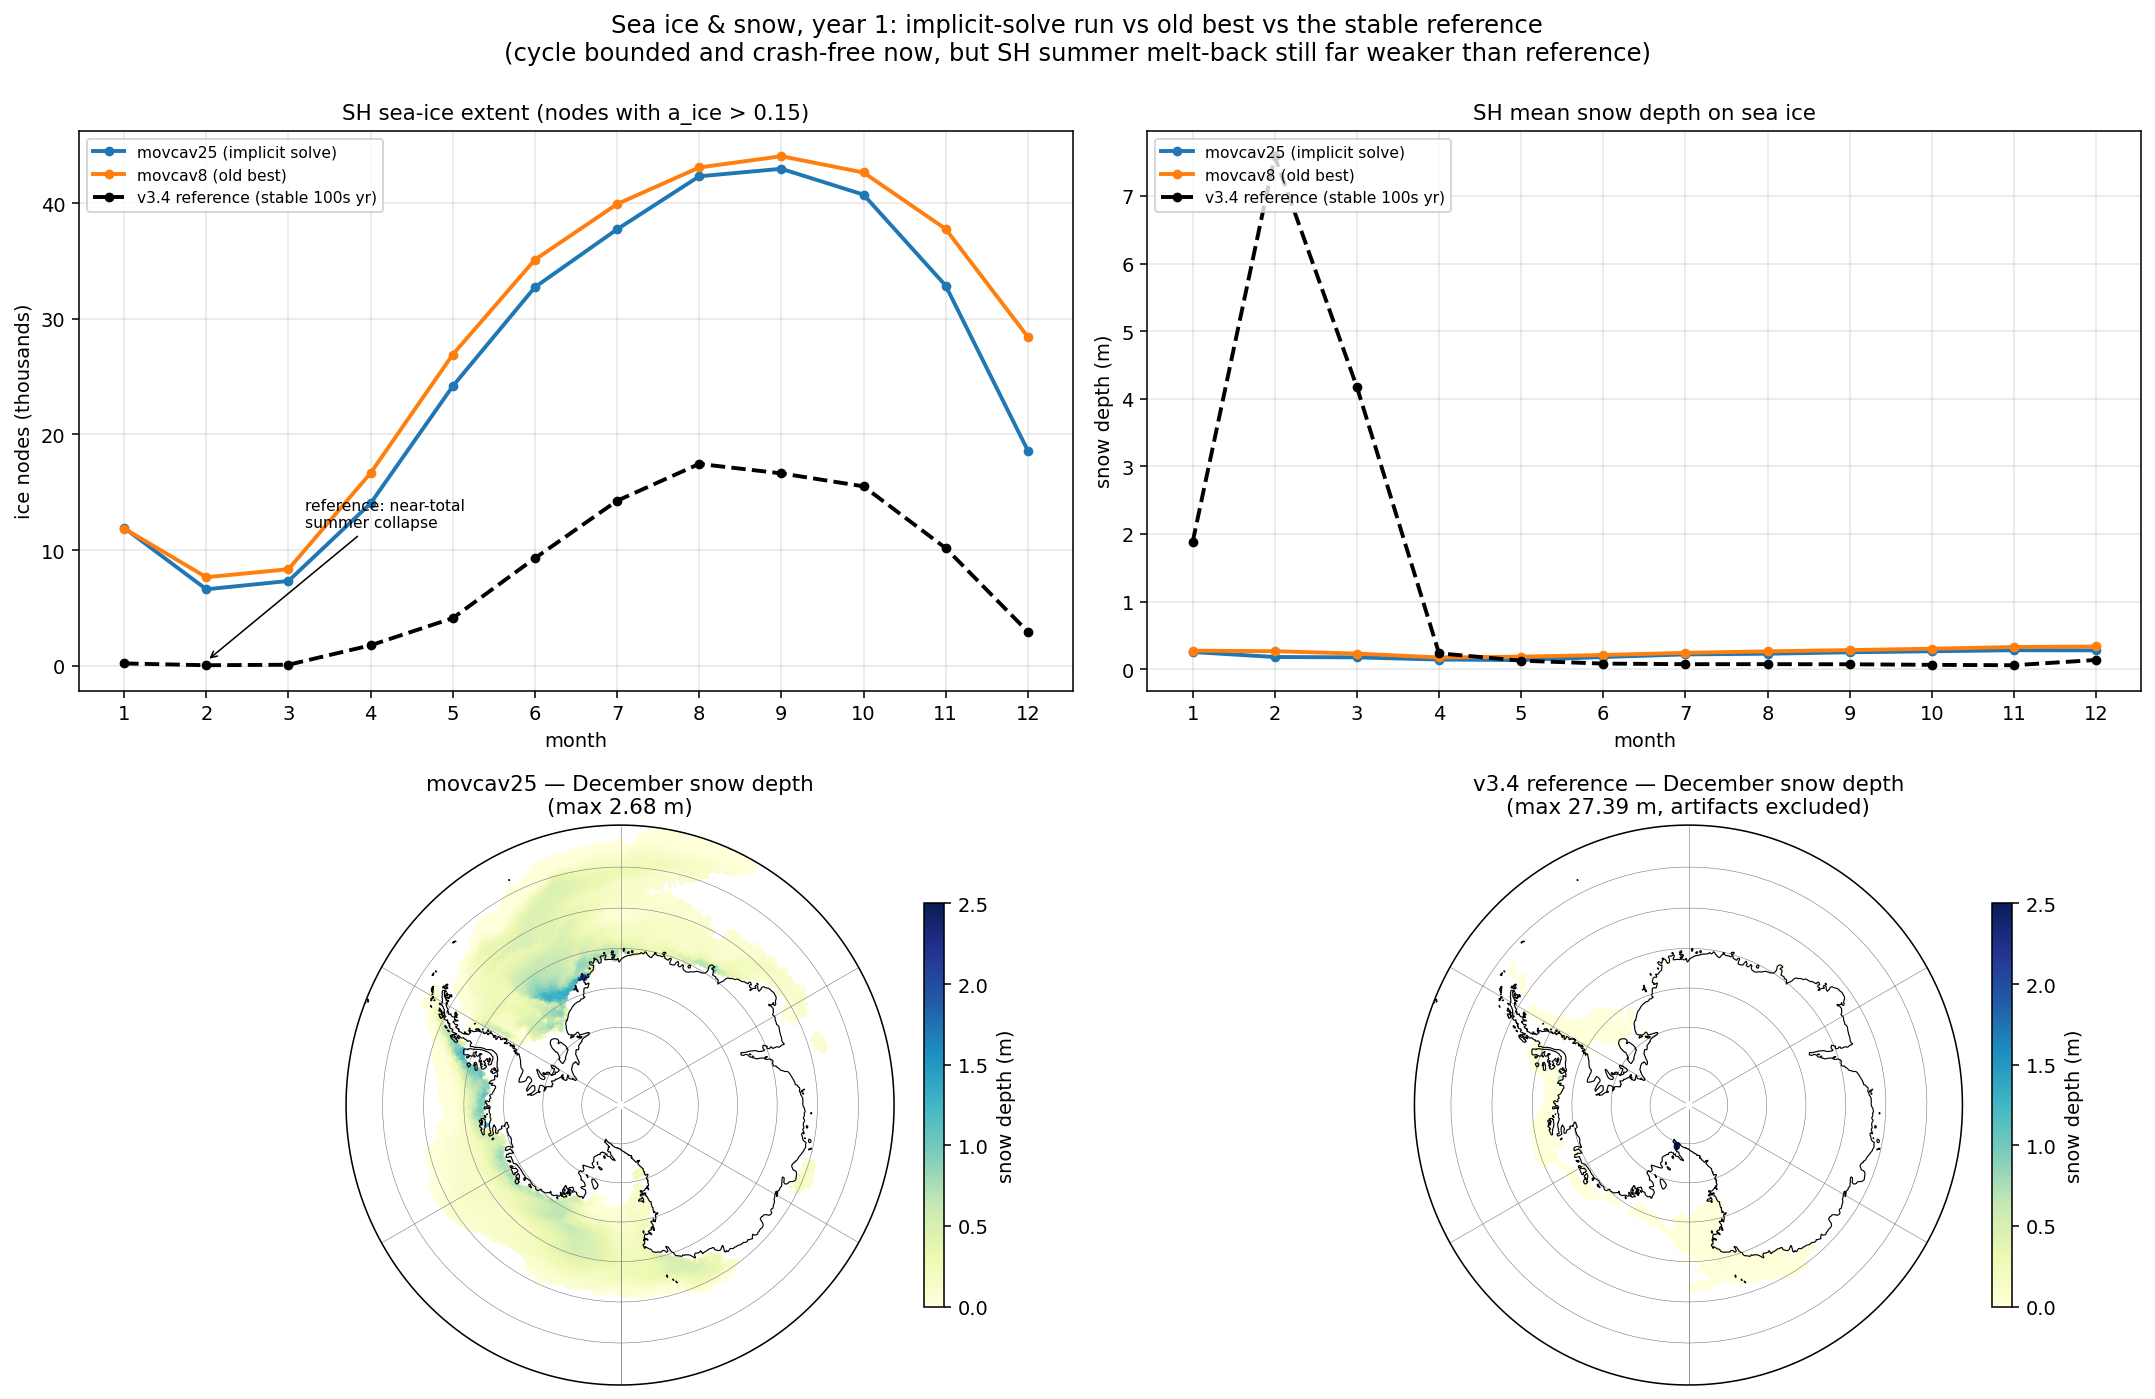
\includegraphics[width=\textwidth]{seaice/snow_ice_mc25_vs_ref.png}
\caption{Year-1 sea ice and snow: implicit-solve run (blue) vs the movcav16-era state (orange) vs
the 500-year-stable v3.4 reference (black dashed). Our runs track each other --- the crash fixes did
not degrade climate --- but the reference collapses its SH ice almost completely each summer while
ours retains $\sim$7k nodes, and its winter pack carries 0.03--0.08\,m of snow against our
0.2--0.3\,m. Bottom maps (same scale): December snow depth --- our thick band hugs the Antarctic
coast; the reference is nearly bare.}
\label{fig:seaiceref}
\end{figure}

\begin{figure}[H]\centering
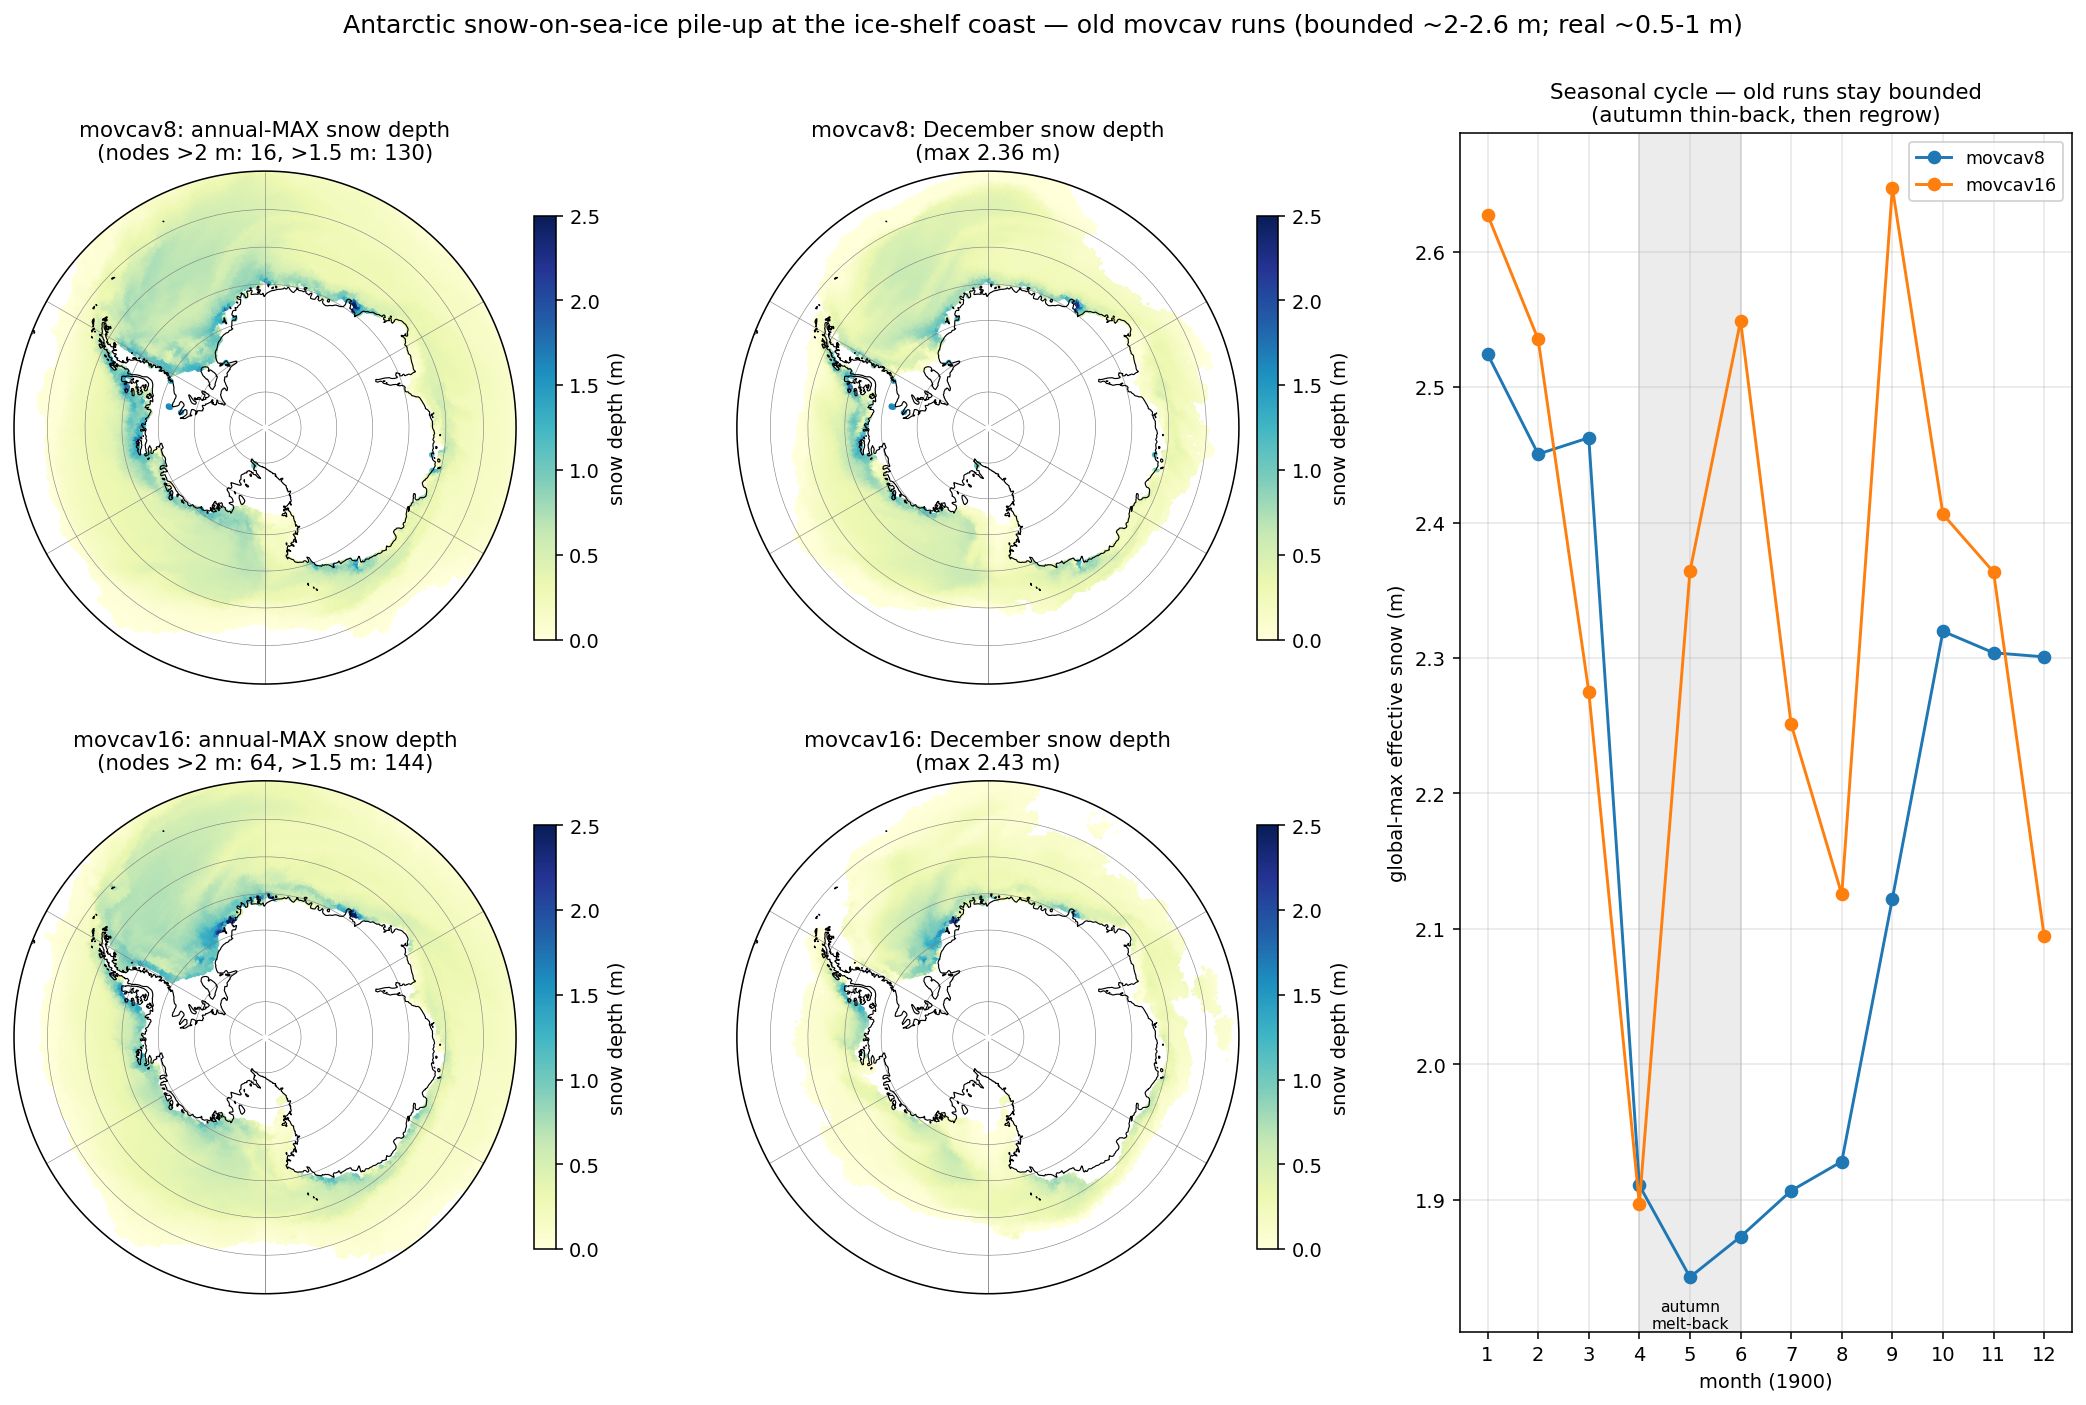
\includegraphics[width=\textwidth]{seaice/snow_extent_movcav.png}
\caption{The extent of the coastal pile-up in the (pre-fix) movcav runs: annual-max and December
snow depth, and the seasonal cycle. The thick snow is a band hugging the ice-shelf front (eastern
Weddell/Fimbul, Amundsen), bounded at 2--2.6\,m by an autumn melt-back. Later runs that lost this
melt-back drifted monotonically to 3.5\,m --- the insulation that raised Bug IV's loop gain.}
\label{fig:snowband}
\end{figure}

The ice-thermodynamics code is byte-identical to the v3.4 reference; the difference is state and
forcing. Ours keeps $\sim$2.5$\times$ the reference's winter SH extent and only a $\sim$6$\times$
summer retreat where the reference manages $\sim$200$\times$ (Fig.~\ref{fig:seaiceref}), and piles
2--3.5\,m of snow against the Antarctic ice-shelf coast (Fig.~\ref{fig:snowband}). Two mitigations
exist: a \emph{clean chunk-1 ice initial state} (reference year-1849 fields index-mapped onto the
submesh via \code{map\_nod.out}, 7 Ronne artifact nodes hybridized; snow max 0.81\,m --- in use
since movcav29), and the coupled slab itself (the pinned-skin era's fictitious equilibria drove a
spurious congelation-growth term). Whether these restore the reference's melt-back is the first
climate question for the post-slab runs; meltponds were checked and are \emph{not} the SH lever (the
\code{hsno>hs1} lockout makes old and corrected schemes identical there).

%======================================================================
\section{Secondary bugs, fixed along the way}

\begin{longtable}{@{}p{6.2cm}p{6.6cm}p{2.2cm}@{}}
\toprule
\textbf{Bug} & \textbf{Fix} & \textbf{Commit} \\
\midrule
\endhead
Remap extrapolated unboundedly below the old seabed (manufactured $-45^\circ$C) when columns
  deepen & take water from the nearest old node wet at that depth & \code{eef4f6db} \\
Sub-ice $\eta$/\code{hbar} kept open-ocean values at newly-sub-ice nodes & zeroed (real bug, not
  the cure) & \code{b17fb5c8} \\
First mesh-change leg read the mother mesh as cavity-free (\code{cavity\_nlvls.out} missing from
  the \code{mother\_as\_old} links) $\Rightarrow$ zeros in newly-wet levels, mstep-1 blowup &
  link the cavity files & functions \\
Same-chunk \code{couple\_in} rerun promoted its own submesh to \code{previous\_submesh}
  (old $=$ new $\Rightarrow$ zeros again) & rerun guard & \code{b9c1e370} \\
OASIS \code{GSSPOS} conservation blowup on near-zero target residuals & \code{gauswgt\_gsmart}
  transform & \code{3e94d4da} \\
namcouple \code{feom} dimension never actually patched (env var from another subjob's shell) &
  fixed variable passing & \code{3cf29e9e} \\
\code{fesom2ice} loaded the static full mesh against submesh output & load the run mesh &
  \code{63cfcc91} \\
\code{previous\_submesh} read but never created & created; plus restart size guard &
  \code{3b44a704} \\
Failed coupling functions did not stop the workflow (backgrounded, observe saw no exit code) &
  \code{.coupling\_failed} sentinel honoured by observe & \code{7953585b} \\
rstos size guard read the wrong dimension & fixed & \code{61c8ed8a} \\
ocp-tool flipped a coastline cell's mask+soil only, leaving an inconsistent surface column &
  masked nearest-neighbour rebuild of the full column & ocp-tool PR\,\#51 \\
Non-short-circuit \code{.and.} read \code{ulevels(0)} at every boundary edge (\code{ice\_maEVP.F90},
  both EVP variants); inside \code{if (use\_cavity)}, so a garbage value decided whether sea-ice
  velocity was zeroed at the cavity--ocean edge & guard \code{edge\_tri(2,ed)>0} separately &
  PR\,\#960 \\
Non-short-circuit \code{.and.} read \code{angles(0)} in the XIOS cell-corner insertion sort
  (\code{io\_xios.F90}); harmless at \code{-O3}, aborts any bounds-checked build at init & split the
  loop test & PR\,\#960 \\
\code{alb} missing from \code{io\_xios\_is\_ice\_field} although declared
  \code{detect\_missing\_value="true"} $\Rightarrow$ sea-ice albedo time-means averaged over open
  water & add \code{'alb'} to the ice-field list & PR\,\#961 \\
\bottomrule
\end{longtable}

\noindent
\textbf{The recurring pattern:} the guards were right and the plumbing around them defeated them ---
a correct refusal followed by an unconditional continue is worse than no guard at all.

%======================================================================
\section{Falsified claims (kept, struck through)}\label{sec:falsified}

\begin{enumerate}
\item \dead{Geostrophically-unbalanced remapped state; initialize changed cells in thermal-wind
  balance.} Failed its own offline gate (discrete $\nabla p$ noisier than NN fill); ships opt-in
  only, off by default.
\item \dead{The sub-ice ssh BC violation is the blowup.} Real bug, fixed, run still died.
\item \dead{The per-leg PISM increment is gentle ($\approx$22\,m mean).} The mean was diluted by the
  98\% unchanged domain; the distribution is wildly skewed (max 923\,m, 1399 fully-opened nodes).
\item \dead{The salt-plume parameterization being off explains the warm cavity.} The spp-off cavity
  is the \emph{coldest} in the CORE3 reference runs; the warm cavity was Bug II.
\item \dead{The native ICMGG causes the mid-run crash family.} The step-0 swap tests proved the
  native, coastline-following surface set is \emph{required} on the submesh (62 difference-zone
  cells cannot initialize otherwise); the mid-run family was Bug IV.
\item \dead{Weighted-ist cures the crash family.} Necessary hygiene for the o2a blend, not
  sufficient: the pinned OIFS skin regenerated the instability from bounded inputs.
\item \dead{The insulation/snow pile-up is the crash root.} It raises the loop gain (and is a real
  climate bias, \S\ref{sec:state}), but the kW events occur on \emph{thin} ice at 49$^\circ$N; the
  clean-ini run crashed identically.
\item \dead{Fragile $\le2$-element coastal slivers cause the Ross-front blowup.} A control
  census killed it: the meshes that ran clean full years carry the same $\sim$3450-node
  fragile count as the crashed one. The cause is increment magnitude, not coastline
  fragility (\S\ref{sec:hygiene}).
\item \dead{The cavity melt gain is $\sim10\times$ too steep (39 vs 1--4\,m/yr/K).} The
  1--4 figure is an integrated-shelf number, not the local exchange sensitivity; the standard
  three-equation scheme gives $\sim$40\,m/yr/K locally, so the measured 39 is correct. The
  melt formula is standard and reproduces the model's melt ($r=0.91$); the excess is in the
  cavity \emph{currents} (\S\ref{sec:melt2}).
\item \dead{The fast cavity currents are an under-damped equilibrium, cured by a tunable
  ice-base drag \code{C\_d\_cavity}.} At the stock drag, chunk-1 and \emph{both} year-long
  cold-start equilibria run at the healthy $\sim$2.6\,cm/s; the fast currents are injected by
  the mesh increment, not a drag deficit (\S\ref{sec:standalone}).
\item \dead{The increment's geometry change injects the spin-up.} A cold start from rest on the
  changed mesh settles to $\sim$2.6\,cm/s --- the new mesh is fine; the carried \emph{remapped
  restart} is what is inconsistent with it (\S\ref{sec:standalone}).
\item \dead{The barotropic margin force $F_x$ (eta$+$sea-ice) drives the spin-up.} The slow
  control carries the same $F_x$ distribution (p90 $\sim7\times10^{-4}$) as the fast runs; the
  step-1 force does not discriminate slow from fast (\S\ref{sec:standalone}).
\item \dead{The leg-start crash is an SSH-RHS explosion: the couple-in hands FESOM a
  transport--geometry mismatch that detonates the external-mode solve.} \code{ssh\_rhs}$=7.1\times10^6$
  is ordinary at a cavity front --- 506 nodes exceed $10^7$, the crash node ranks 143rd of 184 pinched
  nodes, and \code{d\_eta} stays $\le1.76$\,m everywhere because the CG solve absorbs it. The fault is
  in the GM streamfunction (\S\ref{sec:bug8}).
\item \dead{The pinched cavity-front peninsula tip drives the blow-up: remapped velocity has nowhere
  to go through the pinched faces.} The pinch is the normal front geometry and its \code{ssh\_rhs}
  signature is unremarkable at the crash node. The pinch \emph{is} implicated, but through
  \code{ulevels\_nod2D\_max} inverting the GM solve range, not through trapped transport
  (\S\ref{sec:bug8}).
\item \dead{The exact zeros in \code{u} and \code{W} seed the tracer explosion via a singular vertical
  operator.} \code{vert\_vel\_ale} runs \emph{before} \code{solve\_tracers\_ale} and the probe after it
  is silent, so \code{W} was computed from a clean \code{UV}. Both zero fields are residue of the
  $(x+y)-y$ cancellation in the GM bolus add/subtract pair --- the chain runs the other way
  (\S\ref{sec:bug8}).
\item \dead{The fix belongs in the restart remap (\code{mo\_remap\_fields.F90}).} The three affected
  elements come out of the remap clean and geometrically identical to the previous cycle (unchanged
  \code{ulevels}/\code{nlevels}, none new); \code{area}/\code{areasvol}, the partition and its halo
  comm arrays are all self-consistent. The defect is in FESOM's GM solver, exposed --- not created ---
  by the moving cavity (\S\ref{sec:bug8}).
\end{enumerate}

%======================================================================
\section{Method notes}

\begin{enumerate}
\item \textbf{Cheap controls first.} The cold start (geometry vs state), running the fix, plotting
  the distribution instead of the mean --- each killed a confident claim in minutes.
\item \textbf{Measurements from a corrupted run are worse than none} (Bug II poisoned Bug I's
  diagnosis for a week).
\item \textbf{``Same code as the stable reference'' localizes nothing by itself} --- the reference
  ran the same FESIM solve for 500 years; the difference was the state and, one layer deeper, a
  switch default that pinned a skin nobody remembered was pinned.
\item \textbf{Instrument both ends of a coupling before theorizing about either.} Receive-side
  logging (ICEDBG) proved the flux was corrupt; send-side decomposition (SENDDBG) named the term
  and the tile state in its first twelve lines. The two probes cost one rebuild each.
\item \textbf{Beware silent fallbacks} (Bug V's \code{isfile()} miss; the \code{-ocean given}
  silent fallback to \code{th}). A fallback on a nonexistent path should say so. The
  \code{NAMMCC} bug (\S\ref{sec:nammcc}) is the same shape: OIFS silently ran on default switches
  and discarded a coupled field for months, visible only in the sea-ice climate.
\item \textbf{\code{oasis3mct.lresume=false} silently destroys throughput.} With it false the
  coupling restart is rebuilt every exchange and the step rate decays $\sim$100$\times$ over a run
  ($0.28\to11.4$\,s/step) --- no single-leg or one-month test is long enough to see it. Use
  \code{lresume=true} from a restart set that carries the current coupled fields (the shared pool
  \code{rst*} predate \code{sit\_feom} and cannot be used with \code{lresume=true} until
  regenerated).
\item \textbf{In a coupled run FESOM is not forcing-driven.} \code{namelist.forcing}'s JRA55-do
  paths are vestigial (standalone only); the ocean surface fluxes come from OIFS through OASIS, so
  the climate is set by the OIFS GHG year (\code{NCMIPFIXYR}: 1990 for \code{develop} here, 1850
  for the a270270 reference), not by the forcing files.
\end{enumerate}

%======================================================================
\section{Assets}

\begin{itemize}
\item Send/receive flux instrumentation: \code{SENDDBG} (OIFS \code{A\_Q\_ice} decomposition +
  tile state), \code{ICEDBG} (FESIM received flux + state at cold nodes), \code{CPLDBG} (OIFS
  ingest bounds) --- all log-only, strip before merging.
\item \code{oasis\_expout\_o2a} runscript flag: every o2a exchange dumped to netcdf
  ($\sim$20$\times$ slowdown; crash-window probes only).
\item Clean chunk-1 ice initial state (\code{prep/clean\_ice\_ini}): reference year-1849 ice fields
  index-mapped to the submesh; \code{map\_nod.out} makes such remaps exact.
\item A 2-minute offline reproducer (standalone FESOM on the PISM-cavity submesh) and a stable
  full-mesh control.
\item \code{validate\_feom\_weights.py}: aborts any leg whose exchange weights are in the wrong
  node ordering --- would have caught Bug II on day one.
\item \code{verify\_balance.py}: offline balance/stability gate for remapped restarts.
\item Chunk-1 artifacts pooled at \code{input/fesom2/pism\_cavity\_ini/} (login-node launches).
\item Face-(iii) probe set (\code{notes/ssh\_rhs\_probes/}): \code{blowup\_uvrhs.py},
  \code{eta\_seam.py}, \code{front\_census.py}, \code{uv\_holes.py}, \code{uniqueness.py},
  \code{inverted\_range.py} (the $\max(\code{ulevels})>\min(\code{nlevels})$ mesh predicate),
  \code{read\_areas.py}, \code{partition\_check.py}, \code{comm\_symmetry.py}. Working notes in
  \code{notes/ssh\_rhs\_leg\_start\_crash.md}.
\item \code{fesom\_meshdiag} (a standalone utility already in the FESOM tree, \code{BUILD\_MESHDIAG=ON})
  dumps \code{area}/\code{areasvol} per level without running the model --- how \S\ref{sec:bug8}
  cleared the control-volume hypothesis.
\item The crash-step blow-up dump \code{fesom.1906.oce.blowup.CRASH1\_KEEP.nc}: a full 3D state at
  \code{mstep}~1. \code{check\_blowup} writes one on every blow-up and it is routinely ignored;
  opening it is what solved face~(iii).
\end{itemize}

\end{document}
